\documentclass[11pt,twoside,twocolumn]{book}

\RequirePackage[left=1in,
                right=.767in,
                top=1in,
                bottom=1in,
                headheight=14bp,
                headsep=9bp,
                columnsep=0.24in,
                footskip=14bp,
                heightrounded]{geometry}

\usepackage{amsmath}
\usepackage{algorithm}
\usepackage{algpseudocode}
\usepackage{bm}
\usepackage{calc}
\usepackage{natbib}
\usepackage{graphicx}
\usepackage{longtable}
\usepackage{caption}
\usepackage[]{titletoc}

%Do not allow a page break to result in a line appearing by itself 
% https://tex.stackexchange.com/questions/4152/how-do-i-prevent-widow-orphan-lines 
\usepackage[all]{nowidow}

\makeindex
\usepackage{setspace}
% uncomment to make double space 
%\doublespacing
\usepackage{etoolbox}
\usepackage{verbatim}

% set up the listings package for highlighting block definitions and input files
\usepackage{listings}
\usepackage{xcolor}
\lstset{
  basicstyle=\footnotesize\ttfamily\color{black},
  numbers=none,
  columns=flexible,
  backgroundcolor=\color{yellow!10},
%  frame=tlbr,
  moredelim=**[is][\color{red}]{@}{@},
}
\lstdefinestyle{blockdefinition}{
  moredelim=**[is][\color{blue}]{@}{@},
  moredelim=**[is][\color{red}]{\$}{\$},
}
%usage: \lstinputlisting[style=blockdefinition]{./mf6ivar/tex/gwf-chd-dimensions.dat}
\lstdefinestyle{inputfile}{
  morecomment=[l]\#,
  backgroundcolor=\color{gray!10},
}
%usage: \lstinputlisting[style=modeloutput]{file.dat}
\lstdefinestyle{modeloutput}{
  backgroundcolor=\color{blue!20},
}

\usepackage{hyperref}
\hypersetup{
    hidelinks,
    pdftitle={MODFLOW 6 -- Description of Input and Output},
    pdfauthor={MODFLOW 6 Development Team},
    pdfsubject={numerical simulation groundwater flow},
    pdfkeywords={groundwater, MODFLOW, simulation},
    pdflang={en-US},
    bookmarksnumbered=true,     
    bookmarksopen=true,         
    bookmarksopenlevel=1,       
    colorlinks=true,
    allcolors={blue},          
    pdfstartview=Fit,           
    pdfpagemode=UseOutlines,
    pdfpagelayout=TwoPageRight
}

\graphicspath{{./Figures/}}
\newcommand{\modflowversion}{mf6.7.0.dev2}
\newcommand{\modflowdate}{May 12, 2025}
\newcommand{\currentmodflowversion}{Version \modflowversion---\modflowdate}


\newcommand{\disclaimer}{\begin{flushleft}\textbf{DISCLAIMER:} This software is preliminary or provisional and is subject to revision. It is being provided to meet the need for timely best science. The software has not received final approval by the U.S. Geological Survey (USGS). No warranty, expressed or implied, is made by the USGS or the U.S. Government as to the functionality of the software and related material nor shall the fact of release constitute any such warranty. The software is provided on the condition that neither the USGS nor the U.S. Government shall be held liable for any damages resulting from the authorized or unauthorized use of the software.\end{flushleft}}

\title{MODFLOW 6 -- Description of Input and Output \\~\\ **PROVISIONAL**}
\author{MODFLOW 6 Development Team}
\date{\currentmodflowversion \\ \vfill \disclaimer}

\newcommand{\mli}[1]{\mathit{#1}}

\urlstyle{rm}

\newcommand{\programname}{MODFLOW 6}

\usepackage{xspace}
\def\tsc#1#2{\csdef{#1}{#2\xspace}}
\tsc{mff}{MODFLOW}
\tsc{mf}{MODFLOW~6}
\tsc{mfpar}{(MODFLOW~6)}

\usepackage{placeins}
\usepackage{float}
\floatstyle{plain}
\newfloat{exampleinput}{H}{exi}
\floatname{exampleinput}{}

\newcommand{\inreferences}{%
\renewcommand{\theequation}{R--\arabic{equation}}%
\setcounter{equation}{0}%
\renewcommand{\thefigure}{R--\arabic{figure}}%
\setcounter{figure}{0}%
\renewcommand{\thetable}{R--\arabic{table}}%
\setcounter{table}{0}%
\renewcommand{\thepage}{R--\arabic{page}}%
\setcounter{page}{1}%
}

\newcounter{appendixno}
\setcounter{appendixno}{0}
\newcommand{\inappendix}{%
\addtocounter{appendixno}{1}%
\renewcommand{\theequation}{\Alph{appendixno}--\arabic{equation}}%
\setcounter{equation}{0}%
\renewcommand{\thefigure}{\Alph{appendixno}--\arabic{figure}}%
\setcounter{figure}{0}%
\renewcommand{\thetable}{\Alph{appendixno}--\arabic{table}}%
\setcounter{table}{0}%
\renewcommand{\thepage}{\Alph{appendixno}--\arabic{page}}%
\setcounter{page}{1}%
}

\renewcommand{\thesection}{}
\renewcommand{\thesubsection}{}
\newcommand{\SECTION}{\section}
\newcommand{\REFSECTION}{\section}

\makeatletter
\renewcommand*\l@section{\@dottedtocline{1}{0em}{1.5em}}
\renewcommand\section{\@startsection {section}{1}{-1em}%
  {-3.5ex \@plus -1ex \@minus -.2ex}%
  {2.3ex \@plus.2ex}%
  {\normalfont\Large\bfseries}}
\def\sectionmark#1{%
      \markright {\MakeUppercase{#1}}}
\makeatother

\makeatletter
\patchcmd{\@verbatim}
  {\verbatim@font}
  {\verbatim@font\footnotesize}
  {}{}
\makeatother

\renewcommand\bibname{References Cited}

\begin{document}
%\makefrontcover

%\makefrontmatter

\onecolumn
\hbadness=10000
\setlength{\parindent}{1.5pc}

\maketitle

\tableofcontents
\listoffigures
\listoftables

\newpage
%Introduction
\newpage
\incchap
\SECTION{Chapter \thechapno. Introduction}
\customlabel{ch:intro}{\thechapno}
\mf is a command line executable program that reads input from ASCII text files, and optionally from binary files.  \mf writes simulation output to ASCII text and binary files.  \mf itself, like its predecessors, does not provide any graphical output, though users may decide to adopt a Graphical User Interface (GUI) for preparing model input and visualizing model output.  This document provides details on the format of the input files and the format of the output files.  Details on the numerical methods and the underlying theory for MODFLOW 6 are described in separate reports \citep{modflow6framework, modflow6gwf, modflow6xt3d, langevin2020hydraulic, modflow6api, modflow6gwt, modflow6csub, langevin2024}.  Instructions for preparing the input or visualizing the output is beyond the scope of this report.


\newpage
\incchap
\SECTION{Chapter \thechapno. Specific Discharge}
\customlabel{ch:spdis}{\thechapno}
%\noindent \textcolor{red}{CHRIS: Does this interpolation use only cell-cell interfaces, or can it include flows across "exterior" cell faces, as well? I'm guessing the former, as is currently the case in XT3D, but if the latter, then some of the wording will need to be updated.}
% The approach has not yet been modified to handle exterior faces, but this is something that we need to do to improve cell-centered velocities on our edges.

A \mf flow simulation calculates the flow of water across all interfaces between cells. The flow reported for a given cell-cell interface is the component of the flow vector normal to the interface. The normal component of the specific discharge ($L/T$), or Darcy velocity, which we shorten here to "velocity," is obtained by dividing the normal component of flow by the interface area. The velocity vector at the center of a cell can then be estimated by interpolating component information from all the interfaces of the cell.

The velocity interpolation scheme presented here is an adaptation and simplification of the gradient interpolation scheme used in the XT3D capability of \mf \citep{modflow6xt3d}. In XT3D, the three-dimensional head-gradient vector is estimated at a point on the interface between two cells using gradient-component information from the connections between each of those two cells and its neighboring cells. In this velocity interpolation scheme, the three-dimensional velocity vector is estimated at the center of a cell using velocity-component information from the cell-cell interfaces of the cell. (The scheme does not currently include velocity-component information from "external" faces of a cell but could be modified to do so.) The assembly of component information and the weighting scheme in the velocity interpolation are similar to those in the XT3D gradient interpolation: the greatest weight is given to component information from points that are closest to the cell center and whose directions are most closely aligned with the desired velocity component. In XT3D, gradient components are initially estimated in a coordinate system aligned with the connection between two cells, whereas in the velocity interpolation the components are estimated directly in $\left( x, y, z \right)$ model coordinates. This simplifies the notation somewhat and, more importantly, allows the $z$ component to be treated separately from the $x$ and $y$ components using information only from the horizontal interfaces of the cell (those along the top or bottom of the cell), which are the only interfaces that provide $z$-component information.

\subsection{Estimating the $z$ Component of Velocity (Specific Discharge)}

The $z$ component of velocity ($L/T$) at the cell center, $v^z$, is estimated by calculating a weighted average of the $z$ components of velocity at the horizontal interfaces of the cell:

\begin{equation}
\label{eqn:vz}
v^z = \sum_{k=1}^{N_H} \phi_k^z v_k^z,
\end{equation}

\noindent where the summation is over the horizontal interfaces of the cell, which are locally indexed by $k = 1, ..., N_H$, $v_k^z$ is the $z$ component of velocity ($L/T$) at horizontal interface $k$, and $\phi_k^z$ is the weight (unitless) assigned to $v_k^z$. (Weights are discussed in detail in the \hyperref[sec:weights]{"Weights"} section below.)

\subsection{Estimating the $x$ and $y$ Components of Velocity (Specific Discharge)}

The development in this section closely parallels the development in equations 9 through 16 in \cite{modflow6xt3d}. The present development has been adapted specifically for interpolation of the velocity vector at a cell center in $\left( x, y, z \right)$ model coordinates and is simplified by the separate treatment of the $z$ component described in the previous section.

The vertical interfaces of a cell (those along the ``sides'' of the cell), which are locally indexed by $i = 1, ..., N_V$, provide normal-component information that is used to estimated the $x$ and $y$ components of the velocity at the cell center. By definition, $v_i^n$, the normal component of velocity ($L/T$) at vertical interface $i$, is related to the three-dimensional velocity vector by

\begin{equation}
\label{eqn:nivi}
\matr{n_i^T} \matr{v_i} = v_i^n,
\end{equation}

\noindent where superscript ``$\matr{T}$'' indicates the transpose, and the left-hand side of equation~\ref{eqn:nivi} is the scalar product (or ``dot product'') of $\matr{n_i}$, the unit vector (unitless) normal to interface $i$, and $\matr{v_i}$, the velocity vector ($L/T$) at interface $i$. Expanding equation~\ref{eqn:nivi} in terms of vector components gives

\begin{equation}
\label{eqn:nivi2}
n_i^x v_i^x + n_i^y v_i^y + n_i^z v_i^z = v_i^n.
\end{equation}

\noindent where $n_i^x$, $n_i^y$, and $n_i^z$ are, respectively, the $x$, $y$, and $z$ components of $\matr{n_i}$, and $v_i^x$, $v_i^y$, and $v_i^z$ are, respectively, the $x$, $y$, and $z$ components of $\matr{v_i}$. Recognizing that $n_i^z = 0$  for a vertical interface and solving equation~\ref{eqn:nivi2} for the $x$ component of velocity gives

\begin{equation}
\label{eqn:vix}
v_i^x = \left ( v_i^n - n_i^y v_i^y \right ) / n_i^x.
\end{equation}

\noindent The expression for $v_i^x$ in equation~\ref{eqn:vix} is based on information solely from vertical interface $i$. However, the $y$ component, $v_i^y$, which appears on the right-hand side of equation~\ref{eqn:vix}, is unknown and cannot be deduced based on information from interface $i$ alone. Therefore, it is assumed that the $y$ component of velocity ($L/T$) at the cell center, $v^y$, which is also unknown at this point but will eventually be estimated, may be substituted into equation~\ref{eqn:vix} as an approximation to $v_i^y$. The $x$ component of velocity ($L/T$) at the cell center, $v^x$, is then estimated by calculating a weighted average of the $x$ components of velocity at all the vertical interfaces:

\begin{equation}
\label{eqn:vx}
v^x = \sum_{i=1}^{N_V} \phi_i^x v_i^x = \sum_{i=1}^{N_V} \frac{\phi_i^x v_i^n}{n_i^x} - \left( \sum_{i=1}^{N_V} \frac{\phi_i^x n_i^y}{n_i^x}  \right ) v^y,
\end{equation}

\noindent where $\phi_i^x$ is the weight (unitless) assigned to $v_i^x$. Analogous consideration of the $y$ component of velocity ($L/T$) at the cell center, $v^y$, produces the weighted average
\begin{equation}
\label{eqn:vy}
v^y = \sum_{i=1}^{N_V} \phi_i^y v_i^y = \sum_{i=1}^{N_V} \frac{\phi_i^y v_i^n}{n_i^y} - \left( \sum_{i=1}^{N_V} \frac{\phi_i^y n_i^x}{n_i^y}  \right ) v^x,
\end{equation}

\noindent where $\phi_i^y$ is the weight (unitless) assigned to $v_i^y$. (Weights are discussed in detail in the \hyperref[sec:weights]{``Weights''} section below.) There are now two equations, \ref{eqn:vx} and \ref{eqn:vy}, that can be solved for the two unknowns, $v^x$ and $v^y$, to give

\begin{equation}
\label{eqn:vxAB}
v^x = \frac{1}{1 - A^{xy} A^{yx}} \sum_{i=1}^{N_V}  \left( B_i^x - A^{xy} B_i^y \right ) v_i^n
\end{equation}

\begin{equation}
\label{eqn:vyAB}
v^y = \frac{1}{1 - A^{xy} A^{yx}} \sum_{i=1}^{N_V}  \left( B_i^y - A^{yx} B_i^x \right ) v_i^n,
\end{equation}

\noindent where

\begin{equation}
\label{eqn:Axy}
A^{xy} = \sum_{i=1}^{N_V} B_i^x n_i^y
\end{equation}

\begin{equation}
\label{eqn:Ayx}
A^{yx} = \sum_{i=1}^{N_V} B_i^y n_i^x,
\end{equation}

\noindent and

\begin{equation}
\label{eqn:Bix}
B_i^x = \frac{\phi_i^x}{n_i^x}
\end{equation}

\begin{equation}
\label{eqn:Biy}
B_i^y = \frac{\phi_i^y}{n_i^y}.
\end{equation}

\noindent Equations~\ref{eqn:vxAB} and~\ref{eqn:vyAB}, with the coefficients given by equations~\ref{eqn:Axy} through~\ref{eqn:Biy}, are the expressions used to estimate the $x$ and $y$ components of the velocity vector at the cell center based on normal-component information at the vertical interfaces of the cell.

\subsection{Weights} \label{sec:weights}

For estimation of the $z$ component of velocity as a weighted average, we define a set of weights (unitless) based on the shortest distance ($L$), $D_k$, from the cell center to each horizontal interface $k$ as follows:

\begin{equation}
\label{eqn:omegaz}
\omega_k^z = 1 - \frac{D_k}{\sum_{m=1}^{N_H} D_m}.
\end{equation}

\noindent Interfaces that are closest to the cell center receive the greatest weights. Before incorporating the weights into equation~\ref{eqn:vz}, we normalize them so they sum to 1:

\begin{equation}
\label{eqn:phiz}
\phi_k^z = \frac{\omega_k^z}{{N_H} - 1} = \frac{1}{{N_H} - 1} \left (1 - \frac{D_k}{\sum_{m=1}^{N_H} D_m} \right ).
\end{equation}

For estimation of the $x$ and $y$ components of velocity, we define a set of weights (unitless) that take into account not only distance from the cell center, but also how closely the normal-component information at each vertical interface aligns with the velocity component ($x$ or $y$) being expressed as a weighted average. For the $x$ component of velocity the weights are

\begin{equation}
\label{eqn:omegax}
\omega_i^x = \left [ 1 - \frac{D_i \left | n_i^x \right | }{\sum_{l=1}^{N_V}{} D_l  \left | n_l^x \right | } \right ] \left | n_i^x \right | = \left [ \frac{\sum_{l=1}^{N_V} D_l  \left | n_l^x \right |  - D_i \left | n_i^x \right | }{\sum_{l=1}^{N_V} D_l  \left | n_l^x \right | } \right ] \left | n_i^x \right |,
\end{equation}

\noindent and for the $y$ component of velocity the weights are

\begin{equation}
\label{eqn:omegay}
\omega_i^y = \left [ 1 - \frac{D_i \left | n_i^y \right | }{\sum_{l=1}^{N_V} D_l  \left | n_l^y \right | } \right ] \left | n_i^y \right | = \left [ \frac{\sum_{l=1}^{N_V} D_l  \left | n_l^y \right | - D_i \left | n_i^y \right | }{\sum_{l=1}^{N_V} D_l  \left | n_l^y \right | } \right ] \left | n_i^y \right |.
\end{equation}

\noindent Interfaces that are closest to the cell center and align most closely with the component direction ($x$ or $y$) for which they are being used receive the greatest weights. The corresponding normalized weights used in equations~\ref{eqn:Bix} and~\ref{eqn:Biy} are:

\begin{equation}
\label{eqn:phix}
\phi_i^x =  \frac{\omega_i^x \left | n_i^x \right | }{\sum_{l=1}^{N_V} \omega_l^x  \left | n_l^x \right | }
\end{equation}

\noindent and

\begin{equation}
\label{eqn:phiy}
\phi_i^y =  \frac{\omega_i^y \left | n_i^y \right | }{\sum_{l=1}^{N_V} \omega_l^y  \left | n_l^y \right | } ,
\end{equation}

\noindent respectively. Substitution of equations~\ref{eqn:omegax} and~\ref{eqn:omegay} into equations~\ref{eqn:phix} and~\ref{eqn:phiy}, followed by substitution of equations~\ref{eqn:phix} and~\ref{eqn:phiy} into equations~\ref{eqn:Bix} and~\ref{eqn:Biy}, and simplification results in the following expressions for the coefficients $B_i^x$ and $B_i^y$:

\begin{equation}
\label{eqn:bx2}
B_i^x =  \frac{\left [ \sum_{l=1}^{N_V} D_l  \left | n_l^x \right |  - D_i \left | n_i^x \right |  \right ] \left | n_i^x \right | \sign (n_i^x)  }{\sum_{j=1}^{N_V} \left [ \sum_{l=1}^{N_V} D_l  \left | n_l^x \right |  - D_j \left | n_j^x \right | \right ] \left | n_j^x \right |  \left | n_j^x \right | }
\end{equation}

\noindent and

\begin{equation}
\label{eqn:bx2}
B_i^y =  \frac{\left [ \sum_{l=1}^{N_V} D_l  \left | n_l^y \right |  - D_i \left | n_i^y \right |  \right ] \left | n_i^y \right | \sign (n_i^y)  }{\sum_{j=1}^{N_V} \left [ \sum_{l=1}^{N_V} D_l  \left | n_l^y \right |  - D_j \left | n_j^y \right | \right ] \left | n_j^y \right |  \left | n_j^y \right | } ,
\end{equation}

\noindent where $\sign (n)$ equals +1, 0, or -1 when $n$ is positive, zero, or negative, respectively.




\newpage
\incchap
\SECTION{Chapter \thechapno. Drain Package Discharge Scaling}
\customlabel{ch:drn}{\thechapno}
In the original release of the \mf Drain (DRN) Package a drain is designed to simulate the effects of agricultural drains, springs, and other features that remove water from the aquifer at a rate proportional to the difference between the head in the aquifer and some fixed head or elevation, called the drain elevation, so long as the head in the aquifer is above that elevation. If, however, the aquifer head falls below the drain elevation, then the drain has no effect on the aquifer. The constant of proportionality is called the drain conductance.  This chapter describes a new feature of the \mf DRN Package that allows the drain conductance to gradually increase from zero to the user-specified value as a function of the simulated groundwater head.

\subsection{Theory}

The standard drain equation in \mf is

\begin{align}
	\label{eqn:bcdrnqout}
    	\mli{Qout}_{nb} = \begin{dcases} 
    		0 &h_{n} \le \mli{HDRN}_{nb} \\
    		\mli{CDRN}_{nb} \left( h_{n} - \mli{HDRN}_{nb} \right) &h_{n} > \mli{HDRN}_{nb}
	\end{dcases} ,
\end{align}

\noindent where $\mli{Qout}_{nb}$ is the flow from the aquifer to drain $nb$ (\ulct), $\mli{CDRN}_{nb}$ is the drain conductance (\ulst), $\mli{HDRN}_{nb}$ is the drain elevation (\ul), and $h_{n}$ is the head in the cell containing the drain (\ul). Equation~\ref{eqn:bcdrnqout} rewritten in terms of flow from the drain into aquifer (\ulct), $\mli{QDRN}$, is

\begin{align}
	\label{eqn:bcdrnqdrn}
    	\mli{QDRN}_{nb} = \begin{dcases} 
    		\mli{CDRN}_{nb} \left( \mli{HDRN}_{nb} - h_{n} \right) &h_{n} > \mli{HDRN}_{nb} \\
    		0 &h_{n} \le \mli{HDRN}_{nb}
	\end{dcases} .
\end{align}

The standard DRN Package has been modified to include the option to scale the drain conductance using either linear or cubic scaling. The modified form of the drain equation (eq.~\ref{eqn:bcdrnqdrn}) with linear scaling is

\begin{equation}
	\label{eqn:bcdrnqoutalt0}
	\mli{QDRN}_{nb} = F_{\mli{DRN}_{nb}} \mli{CDRN}_{nb} \left( \mli{ZDRN}_{nb} - h_{n} \right) ,
\end{equation}

\noindent where $\mli{ZDRN}_{nb}$ is the elevation at which drainage discharge begins (\ul), and $F_{\mli{DRN}_{nb}}$ is the linear scaling function (unitless), which accounts for how the conductance of the drain changes with changes in head. Conceptually, the drain conductance changes because the area through which flow occurs depends on the head. The area through which flow occurs increases as the head at the drain increases. The linear scaling function is defined as

\begin{equation}
	\begin{aligned}
		\label{eqn:bcdrnFC}
		F_{\mli{DRN}_{nb}} = \begin{dcases} 
			0 &\phantom{0 <} \Delta h_{n,nb}^{r} \le 0 \\
			\Delta h_{n,nb}^{r}  &0 < \Delta h_{n,nb}^{r} < 1 \\
			1 &\phantom{0 <} \Delta h_{n,nb}^{r} \ge 1
		\end{dcases} ,
	\end{aligned}
\end{equation}

\noindent where $\mli{DDRN}_{nb}$ is the drainage depth (\ul) and the relative drain head difference (\ul) is defined as

\begin{equation}
	\label{eqn:reldrainheaddiff}
	\Delta h_{n,nb}^{r} \equiv \frac{h_n - \mli{ZDRN}_{nb}}{\left| \mli{DDRN}_{nb} \right|} .
\end{equation}

\noindent The elevation at which drainage begins, $\mli{ZDRN}_{nb}$ depends on whether the drainage depth, $\mli{DDRN}_{nb}$, is positive or negative and is calculated as

\begin{align}
	\label{eqn:bcdrnZDRN}
	\mli{ZDRN}_{nb} = \begin{dcases}
		\mli{HDRN}_{nb} - \left| \mli{DDRN}_{nb} \right| &\mli{DDRN}_{nb} < 0, \\
		\mli{HDRN}_{nb} &\mli{DDRN}_{nb} \ge 0
    	\end{dcases} .
\end{align}

\noindent If $\mli{DDRN}_{nb}$ is positive, $\mli{ZDRN}_{nb}$ is the drain elevation just as it is in the standard formulation. If $\mli{DDRN}_{nb}$ is negative, $\mli{ZDRN}_{nb}$ is the drain elevation plus the (negative) drainage depth. If $\mli{DDRN}_{nb}$ is zero, the standard formulation is used. The linear scaling function ($F_{\mli{DRN}_{nb}}$) is shown in figure~\ref{fig:drndischscalef}.

\begin{figure}[!ht]
	\begin{center}
	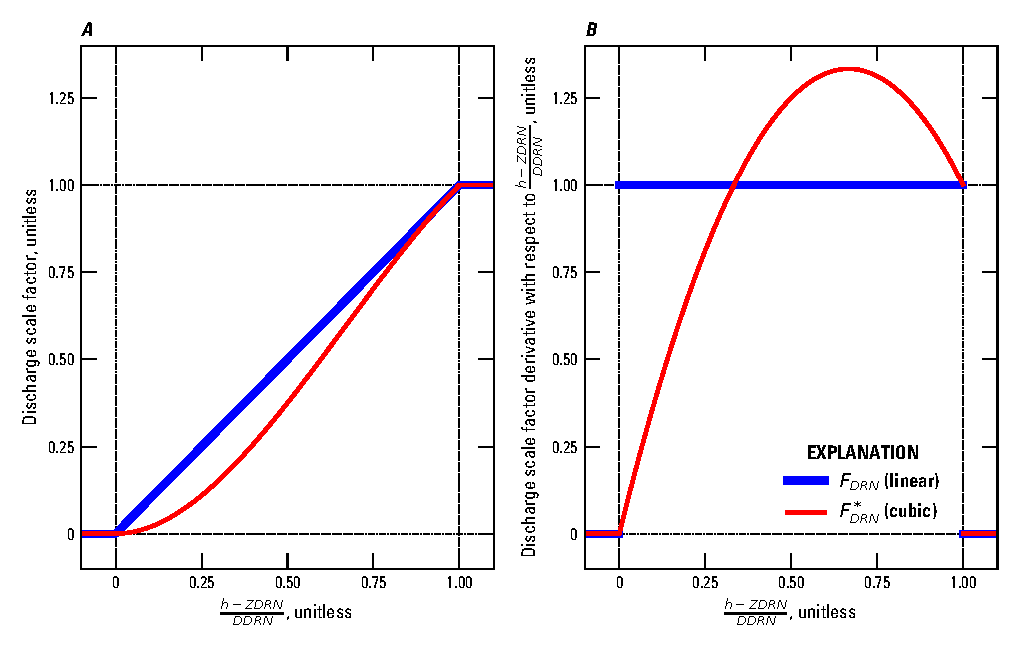
\includegraphics{./Figures/DischargeScaleFactor.pdf}
	\caption[Graphs showing combined linear and cubic scaling functions for drain discharge and the derivatives of the linear and cubic scaling fraction functions]{Graphs showing combined linear and cubic scaling functions for drain discharge and the derivatives of the linear and cubic scaling fraction functions. \textit{A}, linear and cubic fraction functions and \textit{B}, derivatives of the linear and cubic scaling functions with respect to the relative drain head difference $\left( \frac{h - \mli{ZDRN}}{\left| \mli{DDRN} \right|} \right)$. The derivative of the linear and cubic scaling functions with respect to $h$ is the product of the derivative with respect to $\frac{h - \mli{ZDRN}}{\left| \mli{DDRN} \right|}$ and $\frac{1}{\mli{DDRN}}$}
	\label{fig:drndischscalef}
	\end{center}
\end{figure}

The linear scaling function varies with head according to equations~\ref{eqn:bcdrnFC} and~\ref{eqn:reldrainheaddiff}. Differentiation of equation~\ref{eqn:bcdrnFC} with respect to $h_n$, with application of the chain rule to account for the variation of $ \Delta h_{n,nb}^{r}$ with respect to $h_n$ in equation~\ref{eqn:reldrainheaddiff}, gives

\begin{equation}
	\label{eqn:bcdrndFC}
	\begin{aligned}
		\frac{\partial F_{\mli{DRN}_{nb}}}{\partial h_n} = \begin{dcases} 
			0 &\phantom{0 <} \Delta h_{n,nb}^{r} \le 0 \\
			\frac{1}{\left| \mli{DDRN}_{nb} \right|}  &0 < \Delta h_{n,nb}^{r} < 1 \\
			1 &\phantom{0 <} \Delta h_{n,nb}^{r} \ge 1
		\end{dcases} ,
	\end{aligned}
\end{equation}

\noindent which is discontinuous in the neighborhood of $h_n = \mli{ZDRN}_{nb}$ and $h_n = \mli{ZDRN}_{nb} - \left| \mli{DDRN}_{nb} \right| $. The derivative of the linear scaled drain discharge (eq.~\ref{eqn:bcdrnqoutalt0}) with respect to $h_n$ is

\begin{equation}
	\label{eqn:bcdrnNRlindqoutalt0}
	\frac{\partial \mli{QDRN}_{nb}}{\partial h_n} = -F_{\mli{DRN}_{nb}} \mli{CDRN}_{nb}  + \frac{\partial F_{\mli{DRN}_{nb}}}{\partial h_n} \mli{CDRN}_{nb} \left( \mli{ZDRN}_{nb} - h_{n} \right) .
\end{equation}

\noindent Substitution of equations ~\ref{eqn:bcdrnFC} and~\ref{eqn:bcdrndFC} into equation~\ref{eqn:bcdrnNRlindqoutalt0} results in

\begin{equation}
	\begin{aligned}
		\label{eqn:bcdrnNRlindQdh}
		\frac{\partial \mli{QDRN}_{nb}}{\partial h_n} = \begin{dcases} 
			0 &\phantom{0 <} \Delta h_{n,nb}^{r} \le 0 \\
			- 2\, \mli{CDRN}_{nb} \, \Delta h_{n,nb}^{r}  &0 < \Delta h_{n,nb}^{r} < 1 \\
			-\mli{CDRN}_{nb} &\phantom{0 <} \Delta h_{n,nb}^{r} \ge 1
		\end{dcases} ,
	\end{aligned}
\end{equation}

\noindent which remains discontinuous in the vicinity of $\mli{ZDRN}_{nb}$.

When the Newton-Raphson formulation is used, discontinuous derivatives can cause non-convergence in the neighborhood of the discontinuity \citep{doi:10.1029/2006WR005195}. To ensure continuous drain discharge derivatives when the Newton-Raphson formulation is used, cubic smoothing of the linear relative drain head difference is used and equation~\ref{eqn:bcdrnqoutalt0} is modified to

\begin{equation}
	\label{eqn:bcdrnNRqoutalt0}
	\mli{QDRN}_{nb}^* = F_{\mli{DRN}_{nb}}^* \mli{CDRN}_{nb} \left( \mli{ZDRN}_{nb} - h_{n} \right) ,
\end{equation}

\noindent where where $F_{\mli{DRN}_{nb}}^*$ is the cubic scaling function. The cubic scaling function is defined as

\begin{equation}
	\begin{aligned}
		\label{eqn:bcdrnFCC}
		F_{\mli{DRN}_{nb}}^* = \begin{dcases} 
			0 & \phantom{0 <} \Delta h_{n,nb}^{r} \le 0 \\
			- \left( \Delta h_{n,nb}^{r} \right)^3  + 2 \left( \Delta h_{n,nb}^{r} \right)^2  & 0 < \Delta h_{n,nb}^{r} < 1 \\
			1 & \phantom{0 <} \Delta h_{n,nb}^{r} \ge 1
		\end{dcases} ,
	\end{aligned}
\end{equation}

\noindent which is continuous in the vicinity of $h_n = \mli{ZDRN}_{nb}$ and $h_n = \mli{ZDRN}_{nb} - \left| \mli{DDRN}_{nb} \right| $ (fig.~\ref{fig:drndischscalef}\textit{A}). The derivative of equation~\ref{eqn:bcdrnFCC} with respect to $h_n$ is

\begin{equation}
	\begin{aligned}
		\label{eqn:bcdrndFCC}
		\frac{\partial F_{\mli{DRN}_{nb}}^*}{\partial h_n} = \begin{dcases} 
			0 & \phantom{0 <} \Delta h_{n,nb}^{r} \le 0 \\
			-\frac{3}{\left| \mli{DDRN}_{nb} \right|} \left( \Delta h_{n,nb}^{r} \right)^2  + \\
			\phantom{-}\frac{4}{\left| \mli{DDRN}_{nb} \right|} \, \Delta h_{n,nb}^{r} & 0 < \Delta h_{n,nb}^{r} < 1 \\
			0 & \phantom{0 <} \Delta h_{n,nb}^{r} \ge 1
		\end{dcases} ,
	\end{aligned}
\end{equation}

\noindent which is discontinuous in the vicinity of $h_n = \mli{ZDRN}_{nb} - \left| \mli{DDRN}_{nb} \right| $ (fig.~\ref{fig:drndischscalef}\textit{B}). The derivative of the cubic scaled drain discharge (eq.~\ref{eqn:bcdrnNRqoutalt0}) with respect to $h$ is

\begin{equation}
	\label{eqn:bcdrnNRdqoutalt0}
	\frac{\partial \mli{QDRN}_{nb}^*}{\partial h} = -F_{\mli{DRN}_{nb}}^* \mli{CDRN}_{nb}  + \frac{\partial F_{\mli{DRN}_{nb}}^*}{\partial h} \mli{CDRN}_{nb} \left( \mli{ZDRN}_{nb} - h_{n} \right) .
\end{equation}

\noindent Substitution of equations~\ref{eqn:bcdrnFCC} and~\ref{eqn:bcdrndFCC} into equation~\ref{eqn:bcdrnNRdqoutalt0} results in 

\begin{equation}
	\begin{aligned}
		\label{eqn:bcdrndQdh}
		\frac{\partial \mli{QDRN}_{nb}^*}{\partial h_n} = \begin{dcases} 
			0 & \phantom{0 <} \Delta h_{n,nb}^{r} \le 0 \\
			-\mli{CDRN}_{nb} \Biggl[ - \left( \Delta h_{n,nb}^{r} \right)^3  + 2 \left( \Delta h_{n,nb}^{r} \right)^2 \Biggr] + \\
			\phantom{-} \mli{CDRN}_{nb} \Biggl[- \frac{3}{\mli{DDRN}_{nb}} \left( \Delta h_{n,nb}^{r} \right)^2  + \Biggr. \\
			\Biggl. \phantom{-\mli{CDRN}_{nb} \Biggl[- } \frac{4}{\mli{DDRN}_{nb}} \left( \Delta h_{n,nb}^{r} \right) \Biggr] \left( \mli{ZDRN}_{nb} - h_{n} \right) & 0 < \Delta h_{n,nb}^{r} < 1 \\
			-\mli{CDRN}_{nb} & \phantom{0 <} \Delta h_{n,nb}^{r} \ge 1
		\end{dcases} ,
	\end{aligned}
\end{equation}

\noindent which is continuous in the vicinity of $h_n = \mli{ZDRN}_{nb}$ and $h_n = \mli{ZDRN}_{nb} - \left| \mli{DDRN}_{nb} \right| $.

\subsection{Example Drain Discharge Scaling Calculations}

An example of the differences between the standard, linearly-scaled, and cubicly-scaled drainage discharge are shown in figure~\ref{fig:drndischdiff}. In this example the elevation that drainage discharge starts ($\mli{ZDRN}$) is set at $\frac{\mli{DDRN}}{2}$ below land surface elevation and drainage discharge is equal for all approaches at $\mli{ZDRN} + \mli{DDRN}$ (fig.~\ref{fig:drndischdiff}\textit{A}). In this conceptual problem, the groundwater head linearly increases from a value less than $\mli{ZDRN}$ to greater than $\mli{ZDRN + DDRN}$ during the simulation, which is presented as the head difference ($h - \mli{ZDRN}$) divided by the drainage depth in figure~\ref{fig:drndischdiff}\textit{B}. The drainage discharge that results from the linear increase in groundwater head using the original-, linear-, and cubic-scaling increases with time as is shown in figure~\ref{fig:drndischdiff}\textit{C} and shows the continuous nature of the linear- and cubic scaled drainage discharge and that all three approaches result in the same drain discharge rate when the relative drain head difference is greater than or equal to one. Figure~\ref{fig:drndischdiff}\textit{D} shows that the cumulative drain discharge for the original drain formulation is 170 to 200 $L^3$ greater than the cubic- and linear-scaled drainage discharge, respectively.

\begin{figure}[!ht]
	\begin{center}
	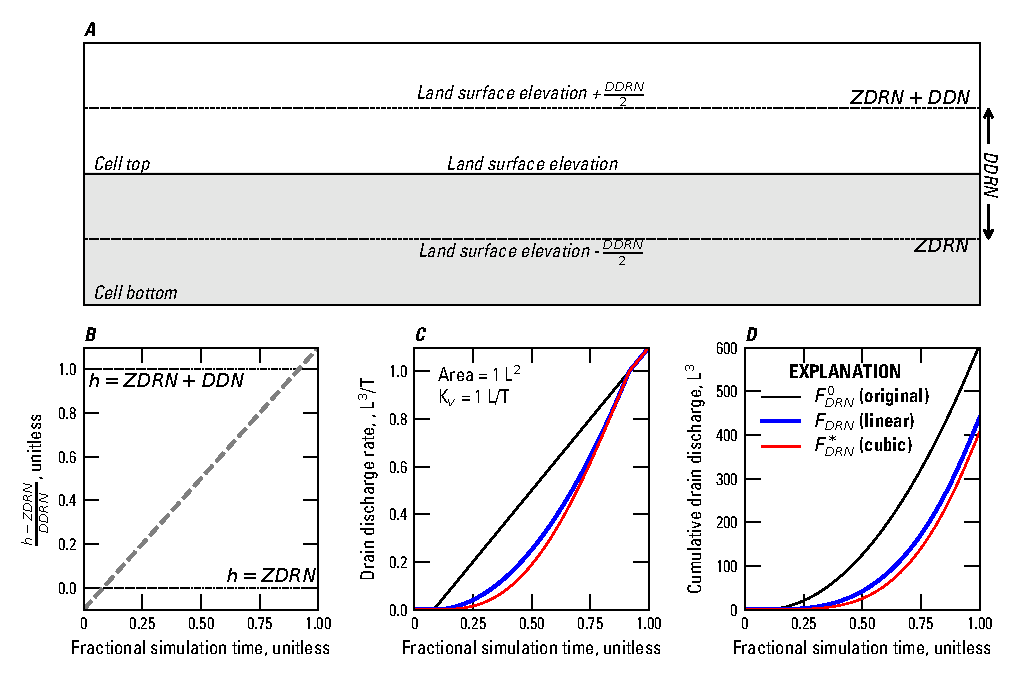
\includegraphics{./Figures/DRNDischargeDifferences.pdf}
	\caption[Graphs showing a conceptual model cell using scaled drain discharge and the relation between the groundwater level and drain discharge]{Graphs showing a conceptual model cell using scaled drain discharge and the relation between the groundwater level and drain discharge. \textit{A}, Conceptual model cell containing a drain cell where drainage discharge starts $\frac{\mli{DDRN}}{2}$ below land surface and is equal $\frac{\mli{DDRN}}{2}$ above land surface for all drain scaling approaches, \textit{B}, conceptual linear groundwater level increases, which are presented as a relative drain head difference, with fractional simulation time, \textit{C}, calculated original, linear, and cubic scaled drainage discharge rates resulting from conceptual groundwater level increases, and \textit{D}, calculated original, linear, and cubic scaled drainage cumulative discharge resulting from conceptual groundwater level increases}
	\label{fig:drndischdiff}
	\end{center}
\end{figure}

\subsection{Incorporation of the modified Drain (DRN) Package into the CVFD Groundwater Flow Equation}

To prepare the CVFD equation for solution using the standard formulation, it is convenient to rearrange the discretized groundwater flow equation for a cell so that all terms containing heads at the end of the current time step are grouped on the left-hand side of the equation, and all terms that are independent of head at the end of the current time step are on the right-hand side of equation 6--1 in \cite{modflow6gwf}. Refer to \cite{modflow6gwf} for additional information on how the groundwater flow equation is formulated in \mf. 

\subsubsection{Standard Formulation}

According to the sign convention in \mf, $\mli{QDRN}_{nb}$ in the groundwater flow equation is defined as a head-dependent flow out of cell $n$, and corresponding terms must be added to the left and right sides of equation~6--1 in \cite{modflow6gwf} for each cell containing a drain. This is accomplished in the modified Drain Package by adding the head-dependent term and the known term in equation~\ref{eqn:bcdrnqoutalt0} to the left- and right-side of equation~6--1 in \cite{modflow6gwf}. The contribution of the modified drain equations to the left-hand side and right-hand sides of the groundwater flow equation are

\begin{equation}
	\label{eqn:qdrnstd}
	\begin{aligned}
		A_{n,n} &\leftarrow A_{n,n} - F_{\mli{DRN}_{nb}} \mli{CDRN}_{nb}   \\
		b_n &\leftarrow b_n - F_{\mli{DRN}_{nb}} \mli{CDRN}_{nb} ZDRN_{nb} ,
	\end{aligned}
\end{equation} 

\noindent where $A_{n,n}$ is the diagonal of the coefficient matrix for cell $n$ and $b_n$ is the right-hand side of the groundwater flow equation for cell $n$. In the case where drainage discharge is not scaled, $F_{\mli{DRN}_{nb}}$ is zero when $h_n$ is less than or equal to $HDRN_{nb}$ and one when $h_n$ is greater than $HDRN_{nb}$, which results in identical behavior as the original drain package formulation.


\subsubsection{Newton-Raphson Formulation}

The modified Newton-Raphson form of equation~\ref{eqn:bcdrnNRqoutalt0} solved in terms of $h$ instead of $\Delta h$  and incorporated into the Newton-Raphson form of the groundwater flow equation \citep[eq. 2--26]{modflow6gwf} is

\begin{equation}
	\label{eqn:nrQout}
	\frac{\partial \mli{QDRN}_{nb}^*}{\partial h_n}  h^k_n  = - \mli{QDRN}_{nb}^* + 
	\frac{\partial \mli{QDRN}_{nb}^*}{\partial h_n}  h^{k-1}_n,
\end{equation} 

\noindent where $h^k_n$ is the head at the end of the current non-linear (picard) iteration and $h^{k-1}_n$ is the head at the start of the current non-linear iteration. Substitution of equations~\ref{eqn:bcdrnNRqoutalt0} and~\ref{eqn:bcdrnNRdqoutalt0} into equation~\ref{eqn:nrQout} results in

\begin{equation}
	\label{eqn:nrQout01}
	\begin{aligned}
		A_{n,n} \leftarrow & A_{n,n} - F_{\mli{DRN}_{nb}}^* \mli{CDRN}_{nb}  + \frac{\partial F_{\mli{DRN}_{nb}}^*}{\partial h} \mli{CDRN}_{nb} \left( \mli{ZDRN}_{nb} - h_{n} \right) \\
		b_n \leftarrow & b_n - F_{\mli{DRN}_{nb}}^* \mli{CDRN}_{nb} \left( \mli{ZDRN}_{nb} - h_{n}^{k-1} \right) \\
		& \phantom{b_n} + \Biggl[ -F_{\mli{DRN}_{nb}}^* \mli{CDRN}_{nb} + \frac{\partial F_{\mli{DRN}_{nb}}^*}{\partial h} \mli{CDRN}_{nb} \left( \mli{ZDRN}_{nb} - h_{n} \right) \Biggr] h^{k-1}_n .
	\end{aligned} 
\end{equation}

\noindent Simplifying the right-hand side contribution in equation~\ref{eqn:nrQout01} results in

\begin{equation}
	\label{eqn:nrQout02}
	b_n \leftarrow b_n - F_{\mli{DRN}_{nb}}^* \mli{CDRN}_{nb} \mli{ZDRN}_{nb} + \Biggl[ \frac{\partial F_{\mli{DRN}_{nb}}^*}{\partial h} \mli{CDRN}_{nb} \left( \mli{ZDRN}_{nb} - h_{n}  \right) \Biggr] h^{k-1}_n .
\end{equation}

\noindent The $F_{\mli{DRN}_{nb}}^* \mli{CDRN}_{nb}$ term in equation~\ref{eqn:nrQout01} and the $F_{\mli{DRN}_{nb}}^* \mli{CDRN}_{nb} \mli{ZDRN}_{nb}$ term in equation~\ref{eqn:nrQout02} are subtracted from the diagonal of the coefficient matrix and the right-hand side of the groundwater-flow equation, respectively, during the standard formulation step for the drain package. The Newton-Raphson formulation for the modified drain package is completed by augmenting the coefficient matrix with the derivative term in equation~\ref{eqn:nrQout01} and adding the second term in equation~\ref{eqn:nrQout02} (the product of a derivative term and the head at the start of the current iteration) to the right-hand side of the groundwater-flow equation. 

\subsection{Use of Drain Discharge Scaling}

A few examples of how the modified drain package can be used to simulate drainage discharge consistent with other \mf packages are given below.

\paragraph{The original drain package formulation with a specified drainage depth value}

Specifying $\mli{DDRN}$ to be 0 results in a drain that behaves the same as the original DRN Package (eq.~\ref{eqn:bcdrnqout}). Using a combination of $\mli{DDRN}$ values set to zero and non-zero values will result in drains with 0 values behaving like the original drain package and others using the scaled drainage discharge approach.

\paragraph{Groundwater seepage from the Unsaturated Zone Flow Package}

The drain package can be used as an alternative to the groundwater seepage option in the Unsaturated Zone Flow (UZF) Package. Specifying a positive $\mli{DDRN}$ value and $\mli{HDRN}_{nb}$ to be $\frac{\mli{DDRN}}{2}$ below the single values specified with the standard DRN Package approach (for example, setting $\mli{DDRN}$ to be at land surface) results in a formulation that is equivalent to the groundwater seepage option available in the UZF Package in \mf \citep{modflow6gwf}. To be consistent with the UZF package, the drain conductance should be calculated as

\begin{equation}
	\label{eqn:uzfcond}
	\mli{CDRN}_{nb} = \frac{K_{v_{nb}} A_n}{\mli{DDRN}_{nb}} ,
\end{equation}

\noindent where $K_{v_{nb}}$ is vertical hydraulic conductivity (\ult) and $A_n$ is the horizontal area of cell $n$ (\uls).


\newpage
\incchap
\SECTION{Chapter \thechapno. Multi-Aquifer Well Package Connection Flow Correction}
\customlabel{ch:maw-qcorr}{\thechapno}
Special considerations are required for flow to convertible cells that can dry and rewet. When flow is between two cells that are wet, the head difference between them creates the driving force for flow. When the downstream cell is dry,
however, a reference elevation can be used instead of the downstream head to express flow between the nodes. The ``perched'' option in the Node Property Flow (NPF) Package can be used to correct downward flow to a partially saturated cell.

The ``flow correction'' option in the Multi-Aquifer Well (MAW) Package implements the same correction as the NPF package ``perched'' option and corrects the flow between a multi-aquifer well connection and a GWF cell. The approach used in the MAW Package is identical to the ``flow-to-dry-cell'' option available in \mfu~\citep{modflowusg}.

\subsection{Multi-Aquifer Well Flow Correction}

When the ``flow correction'' option is enabled, flow to a well from a GWF cell based on equation 7--50 in \cite{modflow6gwf} is

\begin{align}
	\label{eqn:mawQ}
	\mli{QMAW}_{\mli{MAW},n} = \begin{dcases}
		S_{\mli{MAW},n} C_{\mli{MAW},n}^0 \left( h_n - e_{\mli{MAW},n} \right) &  \mli{HMAW}_i < e_{\mli{MAW},n} \\
		S_{\mli{MAW},n} C_{\mli{MAW},n}^0 \left( h_n - \mli{HMAW}_{i} \right) & \mli{HMAW}_i \ge e_{\mli{MAW},n}
	\end{dcases} ,
\end{align}

\noindent where $S_{\mli{MAW},n}$ is the well screen saturation (unitless), $C_{\mli{MAW},n}^0$ is the saturated well conductance (\ulst), $h_n$ is the head in cell $n$ (\ul), $e_{\mli{MAW},n}$ is the reference elevation for the well connection (\ul), and $\mli{HMAW}_{i}$ is the head in well $i$ (\ul). The reference elevation for the well connection is defined to be

\begin{equation}
	\label{en}
	e_{\mli{MAW},n} = \begin{dcases}
		\mli{BOT}_n &  \mli{BOT}_n > \mli{BOT}_{\mli{MAW},n} \\
		\mli{BOT}_{\mli{MAW},n} &  \mli{BOT}_{\mli{MAW},n} > \mli{BOT}_n
	\end{dcases} ,
\end{equation}

\noindent where $\mli{BOT}_n$ is the bottom of cell $n$ (\ul) and $\mli{BOT}_{\mli{MAW},n}$ is the bottom of the well screen for the connection of well $i$ to cell $n$ (\ul). For the case where the head in cell $n$ is less than $e_{\mli{MAW},n}$, flow from a well to a GWF cell is

\begin{align}
	\label{eqn:mawQc2}
	\mli{QMAW}_{\mli{MAW},n} = \begin{dcases}
		S_{\mli{MAW},n} C_{\mli{MAW},n}^0 \left( e_{\mli{MAW},n} - \mli{HMAW}_{i}  \right) &  h_n < e_{\mli{MAW},n} \\
		S_{\mli{MAW},n} C_{\mli{MAW},n}^0 \left( h_n - \mli{HMAW}_{i} \right) & h_m \ge e_{\mli{MAW},n}
	\end{dcases} .
\end{align}

\subsection{Incorporation of the Flow Correction into the CVFD Groundwater Flow Equation}
Multi-aquifer well flow terms are incorporated into the CVFD flow equation \citep[eq. 6--1]{modflow6gwf} based on whether the standard or Newton-Raphson formulation is being used. The details of how the multi-aquifer well flow correction terms are incorporated into the CVFD flow equation is described below.

\subsubsection{Standard Formulation}

The terms in the standard flow equation for all groundwater cells connected to a multi-aquifer well $i$ based on \citep[eq. 7--55]{modflow6gwf} is

\begin{equation}
	\label{mawStdFlow}
	\sum\limits_{n \in \mli{MAW}_{i}}^{} S_{\mli{MAW},n} C_{\mli{MAW},n}^{0} \left( h_{n} - \mli{HMAW}_{i} \right) = 0 .
\end{equation}

\noindent To implement the flow correction, equation~\ref{eqn:mawQ} is modified to

\begin{align}
	\label{eqn:mawQfdc}
	\mli{QMAW}_{\mli{MAW},n} = S_{\mli{MAW},n} C_{\mli{MAW},n}^0 \left( h_n - \mli{HMAW}_{i} \right) + S_{\mli{MAW},n} C_{\mli{MAW},n}^0 \left( \mli{HMAW}_{i} - \overline{h}_{\mli{MAW},n} \right),
\end{align}

\noindent where $\overline{h}_{\mli{MAW},n}$ is a function that transitions between the head at the downstream node, $\mli{HMAW}_{i}$ in this case, and reference elevation $e_{\mli{MAW},n}$. The downstream head transition function used to correct the multi-aquifer flow for a connection is calculated as

\begin{align}
	\label{eqn:maw-hbar}
	\overline{h}_{\mli{MAW},n} = \begin{dcases}
		e_{\mli{MAW},n} &  h_{ds} < e_{\mli{MAW},n} \\
		h_{ds} & h_{ds} \ge e_{\mli{MAW},n}
	\end{dcases} ,
\end{align}

\noindent where $h_{ds}$ is head in the downstream node (\ul), which is the minimum of $\mli{HMAW}_{i}$ and $h_n$. The relation between the downstream head and $\overline{h}_{\mli{MAW},n}$ is shown in figure~\ref{fig:mawhbar}.

\begin{figure}[!ht]
	\begin{center}
	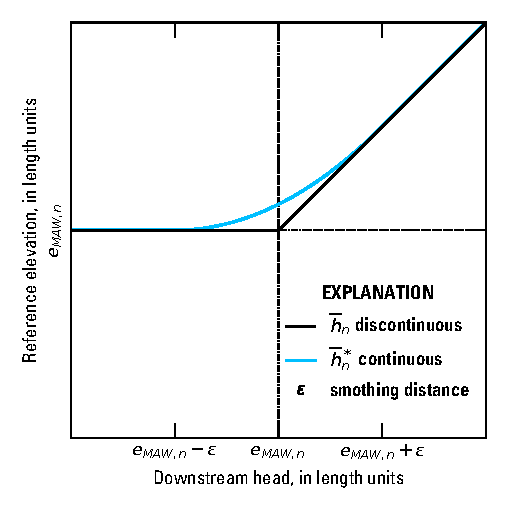
\includegraphics{./Figures/MAWDischargeCorrection.pdf}
	\caption[Graph showing the downstream head transition functions used to correct the multi-aquifer flow for a connection]{Graph showing the discontinuous (eq.~\ref{eqn:maw-hbar}) and continuous (eq.~\ref{eqn:maw-chbar})  downstream head transition function used to correct the multi-aquifer flow for a connection as it transitions from saturated to partially saturated conditions. The interval over which the smoothing occurs, $\epsilon$, is also shown}
	\label{fig:mawhbar}
	\end{center}
\end{figure}

Similarly, when $h_n$ is the downstream node equation~\ref{eqn:mawQc2} is modified to

\begin{align}
	\label{eqn:mawQfdc2}
	\mli{QMAW}_{\mli{MAW},n} = S_{\mli{MAW},n} C_{\mli{MAW},n}^0 \left( h_n - \mli{HMAW}_{i} \right) + S_{\mli{MAW},n} C_{\mli{MAW},n}^0 \left( \overline{h}_{\mli{MAW},n} - h_n \right),
\end{align}

The first term on the right hand side of equations~\ref{eqn:mawQfdc} and~\ref{eqn:mawQfdc2} ($S_{\mli{MAW},n} C_{\mli{MAW},n}^0$) are added to the coefficient matrix used to solve the coupled groundwater and multi-aquifer well flow equations as part of the standard MAW package formulation \citep[eq. 7--55]{modflow6gwf}. The flow correction is made by subtracting the second term on the right hand side of equations~\ref{eqn:mawQfdc} and~\ref{eqn:mawQfdc2} from the right had side of equation 6--1 in \cite{modflow6gwf}. In the case where $\mli{HMAW}_{i}$ and $h_n$ are both greater than $e_{\mli{MAW},n}$, the second term on the right hand side of equations~\ref{eqn:mawQfdc} and~\ref{eqn:mawQfdc2} is equal to zero, which results in a equation identical to equation~\ref{mawStdFlow} for a single connection.


\subsubsection{Newton-Raphson Formulation}

The modified Newton-Raphson form of equation~\ref{mawStdFlow} solved for a single connection in terms of $h$ instead of $\Delta h$  and incorporated into the Newton-Raphson form of the groundwater flow equation \citep[eq. 2--26]{modflow6gwf} is

\begin{equation}
	\label{eqn:nrMawQ}
	\begin{aligned}
		\frac{\partial \mli{QMAW}_{\mli{MAW},n}}{\partial \mli{HMAW}_i}  \mli{HMAW}_i^k + &\frac{\partial \mli{QMAW}_{\mli{MAW},n}}{\partial h_n}  h^k_n = - \mli{QMAW}_{\mli{MAW},n} + \\
		&\frac{\partial \mli{QMAW}_{\mli{MAW},n}}{\partial \mli{HMAW}_i}  \mli{HMAW}_i^{k-1} +  \frac{\partial \mli{QMAW}_{\mli{MAW},n}}{\partial h_n}  h^{k-1}_n ,
	\end{aligned}
\end{equation}

\noindent where $\mli{HMAW}_i^k$ and $h^k_n$ are the heads at the end of the current non-linear (picard) iteration and $\mli{HMAW}_i^{k-1}$ and $h^{k-1}_n$ are the head at the start of the current non-linear iteration.

When the Newton-Raphson formulation is used, discontinuous derivatives can cause non-convergence in the neighborhood of the discontinuity \citep{doi:10.1029/2006WR005195}. As a result, the discontinuous well screen saturation ($S_{\mli{MAW},n}$) in equations~\ref{eqn:mawQfdc} and~\ref{eqn:mawQfdc2} is replaced by a quadratically smoothed well screen saturation ($S_{\mli{MAW},n}^*$ -- eq. 4--5 in \cite{modflow6gwf}). The discontinuous downstream head transition function ($\overline{h}_{\mli{MAW},n}$, eq.~\ref{eqn:maw-hbar}) in equations~\ref{eqn:mawQfdc} and~\ref{eqn:mawQfdc2} is also replaced by

\begin{align}
	\label{eqn:maw-chbar}
	\overline{h}_{\mli{MAW},n}^* = \begin{dcases}
		e_{\mli{MAW},n} &  h_{ds} - e_{\mli{MAW},n} < -\epsilon \\
		\frac{( h_{ds} - e_{\mli{MAW},n} )^2}{4 \epsilon} + \frac{( h_{ds} - e_{\mli{MAW},n} )}{2} + \frac{\epsilon}{4} + e_{\mli{MAW},n}  & -\epsilon < h_{ds} - e_{\mli{MAW},n} < +\epsilon \\
		h_{ds} & h_{ds} - e_{\mli{MAW},n} \ge +\epsilon
	\end{dcases} ,
\end{align}

\noindent where $\epsilon$ is the interval over which the head transition function is smoothed. The relation between the downstream head and $\overline{h}^*_{\mli{MAW},n}$ is shown in figure~\ref{fig:mawhbar}. Simplification of equations~\ref{eqn:mawQfdc} and~\ref{eqn:mawQfdc2} results in

\begin{align}
	\label{eqn:mawQNRc}
	\mli{QMAW}_{\mli{MAW},n} = S_{\mli{MAW},n}^* C_{\mli{MAW},n}^0 \left( h_n - \overline{h}^*_{\mli{MAW},n} \right)
\end{align}

\noindent and

\begin{align}
	\label{eqn:mawQNRc2}
	\mli{QMAW}_{\mli{MAW},n} = S_{\mli{MAW},n}^* C_{\mli{MAW},n}^0 \left( \overline{h}^*_{\mli{MAW},n} - \mli{HMAW}_{i} \right)
\end{align}

\noindent when $\mli{HMAW}_i$ and $h_n$ are the downstream heads, respectively. The derivatives of equation~\ref{eqn:mawQNRc} with respect to $h_n$ and $\mli{HMAW}_i$ are

\begin{equation}
	\label{eqn:nrMawdQdh1}
	\frac{\partial \mli{QMAW}_{\mli{MAW},n}}{\partial \mli{HMAW}_i} =  -S_{\mli{MAW},n}^* C_{\mli{MAW},n}^0 \frac{\partial \overline{h}^*_{\mli{MAW},n}}{{\partial \mli{HMAW}_i}}
\end{equation}

\noindent and

\begin{equation}
	\label{eqn:nrMawdQdhmaw1}
	\frac{\partial \mli{QMAW}_{\mli{MAW},n}}{\partial h_n} = S_{\mli{MAW},n}^* C_{\mli{MAW},n}^0 + \frac{\partial S_{\mli{MAW},n}^*}{\partial h_n} C_{\mli{MAW},n}^0 \left( h_n - \overline{h}^*_{\mli{MAW},n} \right) ,
\end{equation}

\noindent respectively. The derivatives of equation~\ref{eqn:mawQNRc2} with respect to $h_n$ and $\mli{HMAW}_i$ are

\begin{equation}
	\label{eqn:nrMawdQdh2}
	\frac{\partial \mli{QMAW}_{\mli{MAW},n}}{\partial \mli{HMAW}_i} =  -S_{\mli{MAW},n}^* C_{\mli{MAW},n}^0 + \frac{\partial S_{\mli{MAW},n}^*}{\partial \mli{HMAW}_i} C_{\mli{MAW},n}^0 \left( \overline{h}^*_{\mli{MAW},n} - \mli{HMAW}_{i} \right)
	\end{equation}

\noindent and

\begin{equation}
	\label{eqn:nrMawdQdhmaw2}
	\frac{\partial \mli{QMAW}_{\mli{MAW},n}}{\partial h_n} =  S_{\mli{MAW},n}^* C_{\mli{MAW},n}^0 \frac{\partial \overline{h}^*_{\mli{MAW},n}}{\partial h_n} .
\end{equation}

The derivative of $\overline{h}^*_{\mli{MAW},n}$ with respect to the downstream head is

\begin{align}
	\label{eqn:maw-cdhbar}
	\frac{\partial \overline{h}^*_{\mli{MAW},n}}{\partial h_{ds}} = \begin{dcases}
		0 &  h_{ds} - e_{\mli{MAW},n} < -\epsilon \\
		\frac{h_{ds} - e_{\mli{MAW},n}}{2 \epsilon} + \frac{1}{2} & -\epsilon < h_{ds} - e_{\mli{MAW},n} < +\epsilon \\
		1 & h_{ds} - e_{\mli{MAW},n} \ge +\epsilon
	\end{dcases} .
\end{align}


\paragraph{Newton-Raphson formulation when $\mli{HMAW}_i$ is the Downstream Head}

The Newton-Raphson form of the equation~\ref{eqn:mawQfdc}, when $\mli{HMAW}_i$ is the downstream head, is formulated by substituting equations~\ref{eqn:mawQNRc}, ~\ref{eqn:nrMawdQdh1}, and ~\ref{eqn:nrMawdQdhmaw1} into equation~\ref{eqn:nrMawQ}, which results in

\begin{equation}
	\label{eqn:nrMawQmawds01}
	\begin{aligned}
		\biggl[ -S_{\mli{MAW},n}^* &C_{\mli{MAW},n}^0 \frac{\partial \overline{h}^*_{\mli{MAW},n}}{{\partial \mli{HMAW}_i}}
 \biggr] \mli{HMAW}_i^k + \\
 		&\biggl[ S_{\mli{MAW},n}^* C_{\mli{MAW},n}^0 + \frac{\partial S_{\mli{MAW},n}^*}{\partial h_n} C_{\mli{MAW},n}^0 \left( h_n^{k-1} - \overline{h}_{\mli{MAW},n}^{*k-1} \right) \biggr]  h^k_n = \\
		&-S_{\mli{MAW},n}^* C_{\mli{MAW},n}^0 \left( h_n^{k-1} - \overline{h}_{\mli{MAW},n}^{*k-1} \right) + \\
		&\biggl[ -S_{\mli{MAW},n}^* C_{\mli{MAW},n}^0 \frac{\partial \overline{h}^*_{\mli{MAW},n}}{{\partial \mli{HMAW}_i}}
 \biggr] \mli{HMAW}_i^{k-1} + \\
 		&\biggl[ S_{\mli{MAW},n}^* C_{\mli{MAW},n}^0 + \frac{\partial S_{\mli{MAW},n}^*}{\partial h_n} C_{\mli{MAW},n}^0 \left( h_n^{k-1} - \overline{h}_{\mli{MAW},n}^{*k-1} \right) \biggr]  h^{k-1}_n .
	\end{aligned}
\end{equation}

\noindent Simplifying equation~\ref{eqn:nrMawQmawds01} results in

\begin{equation}
	\label{eqn:nrMawQmawds02}
	\begin{aligned}
		\biggl[ -S_{\mli{MAW},n}^* &C_{\mli{MAW},n}^0 \frac{\partial \overline{h}^*_{\mli{MAW},n}}{{\partial \mli{HMAW}_i}}
 \biggr] \mli{HMAW}_i^k + \\
 		&\biggl[ S_{\mli{MAW},n}^* C_{\mli{MAW},n}^0 + \frac{\partial S_{\mli{MAW},n}^*}{\partial h_n} C_{\mli{MAW},n}^0 \left( h_n^{k-1} - \overline{h}_{\mli{MAW},n}^{*k-1} \right) \biggr]  h^k_n = \\
		&S_{\mli{MAW},n}^* C_{\mli{MAW},n}^0 \overline{h}_{\mli{MAW},n}^{*k-1} + \biggl[ -S_{\mli{MAW},n}^* C_{\mli{MAW},n}^0 \frac{\partial \overline{h}^*_{\mli{MAW},n}}{{\partial \mli{HMAW}_i}}
 \biggr] \mli{HMAW}_i^{k-1} + \\
 		&\biggl[ \frac{\partial S_{\mli{MAW},n}^*}{\partial h_n} C_{\mli{MAW},n}^0 \left( h_n^{k-1} - \overline{h}_{\mli{MAW},n}^{*k-1} \right) \biggr]  h^{k-1}_n .
	\end{aligned}
\end{equation}

\noindent To complete the Newton-Raphson formulation the terms added to the coefficient matrix and right-hand side during the standard formulation step (eq.~\ref{eqn:mawQfdc}) are modified by adding

\begin{equation}
	\label{eqn:nrMawdsdiag}
	S_{\mli{MAW},n}^* C_{\mli{MAW},n}^0 \left( 1 - \frac{\partial \overline{h}^*_{\mli{MAW},n}}{{\partial \mli{HMAW}_i}} \right)
\end{equation}

\noindent to the diagonal position in the row for multi-aquifer well $i$, adding

\begin{equation}
	\label{eqn:nrMawdsoffd}
	\frac{\partial S_{\mli{MAW},n}^*}{\partial h_n} C_{\mli{MAW},n}^0 \left( h_n - \overline{h}^*_{\mli{MAW},n} \right)
\end{equation}

\noindent to the off-diagonal position for GWF cell $n$ in the row for multi-aquifer well $i$, and adding

\begin{equation}
	\label{eqn:nrMawdsrhs}
	S_{\mli{MAW},n}^* C_{\mli{MAW},n}^0 \left( 1 - \frac{\partial \overline{h}^*_{\mli{MAW},n}}{{\partial \mli{HMAW}_i}} \right) \mli{HMAW}_i^{k-1} + \frac{\partial S_{\mli{MAW},n}^*}{\partial h_n} C_{\mli{MAW},n}^0 \left( h_n - \overline{h}^*_{\mli{MAW},n} \right) h_n^{k-1}
\end{equation}

\noindent to the right-hand side in the row for multi-aquifer well $i$. The $\left( 1 - \frac{\partial \overline{h}^*_{\mli{MAW},n}}{{\partial \mli{HMAW}_i}} \right)$ term in equation~\ref{eqn:nrMawdsdiag} removes the $-S_{\mli{MAW},n}^* C_{\mli{MAW},n}^0$ term added during standard formulation step and correctly adds the $-S_{\mli{MAW},n}^* C_{\mli{MAW},n}^0 \frac{\partial \overline{h}^*_{\mli{MAW},n}}{{\partial \mli{HMAW}_i}}$ term. The row for the connected groundwater cell (row $n$) is also modified by subtracting equations~\ref{eqn:nrMawdsdiag}, ~\ref{eqn:nrMawdsoffd}, and~\ref{eqn:nrMawdsrhs} from the off-diagonal (column corresponding to multi-aquifer well $i$), diagonal, and right-hand side, respectively.

\paragraph{Newton-Raphson formulation when $h_n$ is the Downstream Head}

The Newton-Raphson form of the equation~\ref{eqn:mawQfdc2}, when $h_n$ is the downstream head, is formulated by substituting equations ~\ref{eqn:mawQNRc2}, ~\ref{eqn:nrMawdQdh2}, and ~\ref{eqn:nrMawdQdhmaw2} into equation~\ref{eqn:nrMawQ}, which results in

\begin{equation}
	\label{eqn:nrMawQgwfds01}
	\begin{aligned}
		\biggl[ -S_{\mli{MAW},n}^* &C_{\mli{MAW},n}^0 + \frac{\partial S_{\mli{MAW},n}^*}{\partial \mli{HMAW}_i} C_{\mli{MAW},n}^0 \left( \overline{h}_{\mli{MAW},n}^{*k-1} - \mli{HMAW}_{i}^{k-1} \right)  \biggr] \mli{HMAW}_i^k + \\
		&\biggl[ S_{\mli{MAW},n}^* C_{\mli{MAW},n}^0 \frac{\partial \overline{h}^*_{\mli{MAW},n}}{\partial h_n} \biggr]  h^k_n = - S_{\mli{MAW},n}^* C_{\mli{MAW},n}^0 \left( \overline{h}_{\mli{MAW},n}^{*k-1} - \mli{HMAW}_{i}^{k-1} \right) + \\
		&\biggl[ -S_{\mli{MAW},n}^* C_{\mli{MAW},n}^0 + \frac{\partial S_{\mli{MAW},n}^*}{\partial \mli{HMAW}_i} C_{\mli{MAW},n}^0 \left( \overline{h}_{\mli{MAW},n}^{*k-1} - \mli{HMAW}_{i}^{k-1} \right) \biggr] \mli{HMAW}_i^{k-1} + \\ &
		\biggl[ S_{\mli{MAW},n}^* C_{\mli{MAW},n}^0 \frac{\partial \overline{h}^*_{\mli{MAW},n}}{\partial h_n} \biggr]  h^{k-1}_n .
	\end{aligned}
\end{equation}

\noindent Simplifying equation~\ref{eqn:nrMawQgwfds01} results in

\begin{equation}
	\label{eqn:nrMawQgwfds02}
	\begin{aligned}
		\biggl[ -S_{\mli{MAW},n}^* &C_{\mli{MAW},n}^0 + \frac{\partial S_{\mli{MAW},n}^*}{\partial \mli{HMAW}_i} C_{\mli{MAW},n}^0 \left( \overline{h}_{\mli{MAW},n}^{*k-1} - \mli{HMAW}_{i}^{k-1} \right)  \biggr] \mli{HMAW}_i^k + \\
		&\biggl[ S_{\mli{MAW},n}^* C_{\mli{MAW},n}^0 \frac{\partial \overline{h}^*_{\mli{MAW},n}}{\partial h_n} \biggr]  h^k_n = - S_{\mli{MAW},n}^* C_{\mli{MAW},n}^0 \overline{h}_{\mli{MAW},n}^{*k-1} + \\
		&\biggl[ \frac{\partial S_{\mli{MAW},n}^*}{\partial \mli{HMAW}_i} C_{\mli{MAW},n}^0 \left( \overline{h}_{\mli{MAW},n}^{*k-1} - \mli{HMAW}_{i}^{k-1} \right) \biggr] \mli{HMAW}_i^{k-1} + \\ &
		\biggl[ S_{\mli{MAW},n}^* C_{\mli{MAW},n}^0 \frac{\partial \overline{h}^*_{\mli{MAW},n}}{\partial h_n} \biggr]  h^{k-1}_n .
	\end{aligned}
\end{equation}

\noindent To complete the Newton-Raphson formulation the terms added to the coefficient matrix and right-hand side during the standard formulation step (eq.~\ref{eqn:mawQfdc2}) are modified by adding

\begin{equation}
	\label{eqn:nrGwfdsdiag}
	\frac{\partial S_{\mli{MAW},n}^*}{\partial \mli{HMAW}_i} C_{\mli{MAW},n}^0 \left( \overline{h}_{\mli{MAW},n}^{*k-1} - \mli{HMAW}_{i}^{k-1} \right)
\end{equation}

\noindent to the diagonal position in the row for multi-aquifer well $i$, adding

\begin{equation}
	\label{eqn:nrGwfdsoffd}
	S_{\mli{MAW},n}^* C_{\mli{MAW},n}^0 \left( \frac{\partial \overline{h}^*_{\mli{MAW},n}}{\partial h_n} - 1\right)
\end{equation}

\noindent to the off-diagonal position for GWF cell $n$ in the row for multi-aquifer well $i$, and adding

\begin{equation}
	\label{eqn:nrGwfdsrhs}
	\frac{\partial S_{\mli{MAW},n}^*}{\partial \mli{HMAW}_i} C_{\mli{MAW},n}^0 \left( \overline{h}_{\mli{MAW},n}^{*k-1} - \mli{HMAW}_{i}^{k-1} \right) \mli{HMAW}_i^{k-1} + S_{\mli{MAW},n}^* C_{\mli{MAW},n}^0 \left( \frac{\partial \overline{h}^*_{\mli{MAW},n}}{\partial h_n} - 1 \right) h^{k-1}_n
\end{equation}

\noindent to the right-hand side in the row for multi-aquifer well $i$. The $\left( \frac{\partial \overline{h}^*_{\mli{MAW},n}}{\partial h_n} - 1 \right)$ term in equation~\ref{eqn:nrGwfdsoffd} removes the $S_{\mli{MAW},n}^* C_{\mli{MAW},n}^0$ term added during standard formulation step and correctly adds the $S_{\mli{MAW},n}^* C_{\mli{MAW},n}^0 \frac{\partial \overline{h}^*_{\mli{MAW},n}}{{\partial h_n}}$ term. The row for the connected groundwater cell (row $n$) is also modified by subtracting equations~\ref{eqn:nrGwfdsdiag}, ~\ref{eqn:nrGwfdsoffd}, and~\ref{eqn:nrGwfdsrhs} from the off-diagonal (column corresponding to multi-aquifer well $i$), diagonal, and right-hand side, respectively.

\newpage
\incchap
\SECTION{Chapter \thechapno. Storage Package Modifications}
\customlabel{ch:sto-mod}{\thechapno}
The \mf Storage (STO) Package simulates the contributions of specific storage and specific yield to the groundwater flow equations. Under confined conditions, in which the head above the top of the cell, storage changes are attributable solely to specific storage. Under unconfined conditions, in which the head is above the bottom but below the top of the cell, storage changes are attributable primarily to specific yield, but the contribution of specific storage is also taken into account.

In the original release of the \mf STO Package, the contribution of specific yield is formulated in terms of hydraulic head in a way that conserves water volume but renders the storage change under unconfined conditions dependent on the vertical datum relative to which heads and elevations are defined. Reexamination of the specific storage contribution in terms of pressure head leads to a revised formulation that eliminates the vertical datum dependence and still honors water conservation. This chapter describes the revised specific storage formulation used in the \mf STO Package.

\subsection{Original Approach}

The specific storage formulation used prior to \mf version 6.1.3 is

\begin{equation}
	\label{eqn:STOeq-orig}
	Q_{SS} = \frac{SC1}{\Delta t} \left(S_{F}^\told h^\told -S_F^t h^{t} \right),
\end{equation}

\noindent where $Q_{SS}$ is the volumetric flow rate from specific storage in the cell ($L^3/T$), $SC1$ is the primary storage coefficient ($L^2$), $\Delta t = t - \told$ is the time step length ($T$), $S_F$ is the fractional saturation of the cell for the previous ($\told$) or current ($t$) time step (unitless), $h$ is the head in the cell for the previous ($\told$) or current ($t$) time step ($L$). The subscript that indicates the cell number has been omitted for clarity. The primary storage coefficient is calculated as 

\begin{equation}
	\label{eqn:STOeq-sc1}
	SC1 = \sps A \Delta z,
\end{equation}

\noindent where $\sps$ is the specific storage coefficient for the cell ($L^{-1}$), $A$ is the horizontal area of the cell ($L^2$), and $\Delta z$ is the cell thickness ($L$) defined by

\begin{equation}
	\label{eqn:cell-thickness}
	\Delta z = TOP - BOT,
\end{equation}
 
\noindent where $TOP$ and $BOT$ are the top and bottom elevations ($L$) of the cell, respectively. The cell saturation is related to the head in the cell by

\begin{align}
	\label{eqn:cell-saturation}
	S_{F} = \begin{dcases}
		1 & h > TOP \\
		\frac{h - BOT}{\Delta z} & BOT < h \le TOP \\
		0 & h \le BOT
	\end{dcases} .
\end{align}

\noindent When the Newton-Raphson formulation is used, the cell saturation in equation~\ref{eqn:cell-saturation} is quadratically smoothed to provide a continuous derivative with respect to head \citep[see][Fig.~4--1 and Eq.~4-5]{modflow6gwf}.

The cell saturation was included in equation~\ref{eqn:STOeq-orig} to scale the primary storage coefficient in proportion to the saturated volume of water in the cell under water-table conditions. However, the formulation in equation~\ref{eqn:STOeq-orig} causes the calculated value of $Q_{SS}$ to depend on the vertical datum, or reference elevation, relative to which heads and elevations are defined. If the vertical datum is changed by an amount $\Delta z_{ref}$ ($L$), all head values change by an amount $-\Delta z_{ref}$, and equation~\ref{eqn:STOeq-orig} becomes

\begin{equation}
	\label{eqn:STOeq-adj}
	Q_{SS} = \frac{SC1}{\Delta t} \left[ S_F^\told \left(h^\told -\Delta z_{ref} \right) - S_F^t \left( h^{t} -\Delta z_{ref} \right) \right] ,
\end{equation}

 \noindent Comparison of equations~\ref{eqn:STOeq-orig} and~\ref{eqn:STOeq-adj} shows that changing the vertical datum by $\Delta z_{ref}$ changes the calculated value of $Q_{SS}$ by

\begin{equation}
	\label{eqn:STOeq-adj-deltaQss}
	\Delta Q_{SS} = \frac{SC1}{\Delta t} \left( S_F^\told - S_F^t \right)  \Delta z_{ref} ,
\end{equation}

\noindent Dependence of $Q_{SS}$ on the vertical datum is not physically realistic and introduces error into the calculated value of $Q_{SS}$.
To illustrate the magnitude of the error that can be introduced, equations~\ref{eqn:STOeq-adj-deltaQss} and~\ref{eqn:STOeq-sc1} were used to calculate $\Delta Q_{SS}$ for a range of cell saturations at times $t$ and $\told$ and cell thicknesses (fig.~\ref{fig:orig-sserror}). For this example, a specific storage value of \SI{1e-5}{\per\meter}, a cell area of 1 \si{\square\meter}, and a time step length of 1 \si{\day} was used in all of the calculations. $\Delta Q_{SS}$ increases as the cell thickness increases or the difference in cell saturations at times $t$ and $\told$ increases.

\begin{figure}
	\begin{center}
	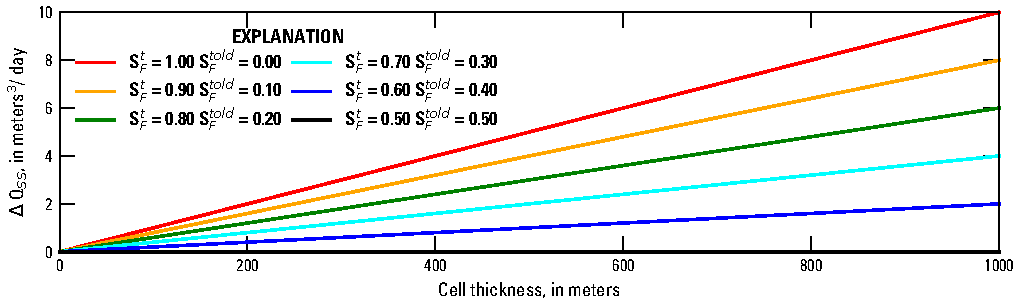
\includegraphics{./Figures/STOSsError.pdf}
	\caption[Graph showing changes in the flow from specific storage that result from changing the vertical datum]{Graph showing changes in the flow from specific storage, $Q_{SS}$, that result from changing the vertical datum from 0 to 1,000 m. The change in $Q_{SS}$ is plotted at a function of cell thickness, $\Delta z$, for various combinations of initial and final cell saturations, $S_F^\told$ and $S_F^t$. In this example, $\sps = 1\times10^{-5}$ m$^{-1}$, $A = 1$ m$^2$, and $\Delta t = 1$ d}
	\label{fig:orig-sserror}
	\end{center}
\end{figure}

A related deficiency of equation~\ref{eqn:STOeq-orig} concerns when a cell is dry either at the beginning ($S_F^\told = 0$) or the end ($S_F^t = 0$) of a time step, in which case the volumetric flow from specific storage equals 

\begin{align}
	\label{eqn:STOeq-def}
	Q_{SS} = \begin{dcases}
		\phantom{-} \frac{SC1}{\Delta t} S_F^\told h^\told & S_F^t = 0 \\
		- \frac{SC1}{\Delta t} S_F^t h^{t} & S_F^\told = 0
	\end{dcases} .
\end{align}

\noindent Equation~\ref{eqn:STOeq-def} can overestimate or underestimate the volumetric flow from specific storage, depending on the values of $h^\told$ and $h^t$, which in turn depend on the vertical datum. For example, in the case of a cell going dry ($S_F^\told > 0$, $S_F^t = 0$), water flows from specific storage, which implies $Q_{SS}$ is positive in sign. Because the cell is initially not dry, the initial cell head, $h^\told$, is above the cell bottom elevation. However, depending on the vertical datum, it is possible that $h^\told$ is negative in sign (with the cell bottom elevation being even more negative). In that case, equation~\ref{eqn:STOeq-def} calculates a negative value for $Q_{SS}$, which is opposite to what is expected on physical grounds.

\subsection{Revised Formulation}

To correct the deficiencies in the original specific storage formulation, the contribution of specific storage to the groundwater flow equation under water-table conditions is reexamined in terms of pressure head, which for a given elevation $z$ is defined as

\begin{equation}
	\label{eqn:pressure-head}
	\psi = h - z.
\end{equation}

\noindent The hydraulic head, $h$, associated with a MODFLOW cell is formally assigned to a point in the cell called the node, which under water-table conditions is at an elevation halfway between the cell bottom and the water table. The water-table elevation is, in turn, equal to the cell head, $h$. Thus, the value of the hydraulic head is the same at the node as it is at the water table, which is consistent with conceptualizing hydaulic head as being constant throughout the saturated portion of the cell. Extending this conceptualization to pressure head via equation~\ref{eqn:pressure-head} implies a linear variation of pressure head between a value of $0$ at the water table and a value of $h - BOT$ at the cell bottom. The revised specific storage formulation is therefore based on linear variation of pressure head with elevation within a cell.

The volumetric water content, $\theta$, at elevation $z$ within a cell is related to pressure head by

\begin{equation}
	\label{eqn:water_content}
	\begin{aligned}
		\theta = 
		\begin{dcases}
			\theta_r & z > h \\
			\sps \psi + S_y + \theta_r  & z \leq h
		\end{dcases},
	\end{aligned}
\end{equation}

\noindent where $\theta_r$ is the specific retention (unitless) and $S_y$ is the specific yield (unitless) in the cell. Integration of equation~\ref{eqn:water_content} from the bottom to the top of the cell gives the total volume of water stored in the cell:

\begin{equation}
	\label{eqn:storage-total-integrated}
	V_S = A \int_{BOT}^{TOP} \theta \, dz = A \int_{BOT}^{\zwts} \sps \psi \, dz + A \int_{BOT}^{\zwts} S_y \, dz + A \int_{BOT}^{TOP} \theta_r \, dz ,
\end{equation}

\noindent where $\zwts$ is the water-table elevation limited by the top elevation of the cell, given by

\begin{equation}
	\label{eqn:zwt}
	\zwts = BOT + \Delta z \, S_F .
\end{equation}

\noindent Assuming $\theta_r$, $S_y$, and $\sps$ are uniform throughout the cell, substitution of equation~\ref{eqn:pressure-head} into equation~\ref{eqn:storage-total-integrated} and evaluation of the integrals gives

\begin{equation}
	\label{eqn:storage-total}
	V_S = S_s A\ \Delta z\, S_F \left( h - \bar{z} \right) + S_y A\ \Delta z\, S_F + \theta_{r} A\ \Delta z ,
\end{equation}

\noindent where $\bar{z}$ is the node elevation (the vertical center of the saturated portion of the cell) given by

\begin{equation}
	\label{eqn:avg-z}
	\begin{aligned}
		\bar{z} = \frac{1}{\zwts - BOT} \int_{BOT}^{\zwts} z \, dz = BOT + \frac{\Delta z}{2} S_F .
	\end{aligned}
\end{equation}

The remainder of this chapter focuses on the contribution of specific storage (the first term on the right-hand side of equation~\ref{eqn:storage-total}) to the change in storage in a cell during a time step. The contribution of specific yield is calculated separately in \mf and remains unchanged by the revised approach described here. The volume of water in specific retention is assumed to be constant and therefore does not contribute to changes in storage.

Substitution of equations~\ref{eqn:STOeq-sc1} and~\ref{eqn:avg-z} into the first term on the right-hand side of equation~\ref{eqn:storage-total} gives the volume of water in compressible storage in the cell,

\begin{equation}
	\label{eqn:storage-ss-final}
	V_{SS} = SC1 \, S_F \left( h - BOT - \frac{\Delta z}{2} S_F \right) .
\end{equation}

\noindent The revised volumetric flow rate from compressible storage is then

\begin{equation}
	\label{eqn:STOeq-rev}
	Q_{SS} = \frac{SC1}{\Delta t} \left[ S_F^\told \left( h^\told - BOT - \frac{\Delta z}{2} S_F^\told \right) - S_F^t \left( h^t - BOT - \frac{\Delta z}{2} S_F^t \right) \right].
\end{equation}

\noindent When a cell is fully saturated ($S_F = 1$) at times $t$ and $\told$, equation~\ref{eqn:STOeq-rev} simplifies to

\begin{equation}
	\label{eqn:STOeq-rev-simp}
	Q_{SS} = \frac{SC1}{\Delta t} \left( h^\told - h^t \right) ,
\end{equation}

\noindent which is identical to the original specific storage formulation under confined conditions in \mf and the specific storage formulation under both confined and unconfined conditions in \mff \citep{modflow2005}.

The revised formulation in equation~\ref{eqn:STOeq-rev} is no longer dependent on the vertical datum because it involves cell saturations, $S_F$, and head differences of the form $h - BOT$, which do not change when the vertical datum changes. In the case of a cell being dry either at the beginning  or the end of a time step, the volumetric flow from specific storage based on the revised formulation equals 

\begin{align}
	\label{eqn:STOeq-def-rev}
	Q_{SS} = \begin{dcases}
		\phantom{-} \frac{SC1}{\Delta t} S_F^\told \left( h^\told - BOT - \frac{\Delta z}{2} S_F^\told \right) & S_F^t = 0 \\
		- \frac{SC1}{\Delta t} S_F^t \left( h^t - BOT - \frac{\Delta z}{2} S_F^t \right) & S_F^\told = 0
	\end{dcases} ,
\end{align}

\noindent which is the revised-formulation counterpart of equation~\ref{eqn:STOeq-def}. It can be deduced from equation~\ref{eqn:cell-saturation} that

\begin{equation}
	\label{eqn:hterm-sign}
	h - BOT - \frac{\Delta z}{2} S_F > 0 \quad \text{if \ $h > BOT$} ,
\end{equation}

\noindent which implies that equation~\ref{eqn:STOeq-def-rev} calculates the correct sign for $Q_{SS}$ when a cell goes dry or resaturates.

\subsection{Incorporation of the Revised Specific Storage Formulation into the CVFD Groundwater Flow Equation}

The approaches used to incorporate the contribution from specific storage into the linear matrix problem that represents the discretized groundwater flow equation are detailed below. When the standard formulation is used, the cell saturation defined in equation~\ref{eqn:cell-saturation} is used without modification. To allow for a smooth transition from dry (water level at or below the bottom of a cell) to fully saturated (water level at or above the top of the cell) conditions when the Newton formulation is used, quadratic smoothing is applied to the cell saturation over a small interval when the water level approaches the top or bottom of a cell, as described in in Eq.~4--5 in \cite{modflow6gwf}. 

\subsubsection{Standard Formulation}

Adding the cell number subscript ``$n$'' to cellwise quantities in equation~\ref{eqn:STOeq-rev} and adding specific storage terms dependent on the current value of head and known terms to the left- and right-hand sides of the discretized groundwater flow equation \citep[eq. 6--1]{modflow6gwf}, respectively, results in

\begin{equation}
	\label{eqn:STOeq-rev-fd}
	\begin{aligned}
		A_{n,n} \leftarrow & A_{n,n} - \frac{SC1_n}{\Delta t} S_{F_n}^\kmo \\
		b_n \leftarrow & b_n - \frac{SC1_n}{\Delta t} \biggl[ S_{F_n}^\told \left( h_n^\told - BOT_n - \frac{\Delta z_n}{2} S_{F_n}^\told \right) +  S_{F_n}^\kmo \left( BOT_n + \frac{\Delta z_n}{2} S_{F_n}^\kmo \right) \biggr],
	\end{aligned}
\end{equation} 

\noindent where $A_{n,n}$ is the diagonal of the coefficient matrix for cell $n$ and $b_n$ is the right-hand side of the groundwater flow equation for cell $n$. A variant of equation~\ref{eqn:STOeq-rev-fd} that tries to take advantage of the fact that

\begin{equation}
	\label{eqn:hterm-WTconditions}
	h_n - BOT_n - \frac{\Delta z_n}{2} S_{F_n} = \frac{1}{2} \left( h_n - BOT_n \right)
\end{equation}

\noindent under water-table conditions (head in the cell below the top of the cell) was also evaluated. However, the form presented in equation~\ref{eqn:STOeq-rev-fd} was found to converge better for the test problems evaluated and to simplify the additional terms added to the left- and right-hand sides of the discretized groundwater equation to complete the Newton-Raphson formulation.

\subsubsection{Newton-Raphson Formulation}

Adding the cell number subscript ``$n$'' to cellwise quantities in equation~\ref{eqn:STOeq-rev} and rearranging the equation to facilitate differentiation with respect to the current value of head, $h_n^t$, results in

\begin{equation}
	\label{eqn:STOeq-rev-2}
	Q_{SS_n} = \frac{SC1_n}{\Delta t} \left[S_{F_n}^\stold \left( h_n^\told - BOT_n - \frac{\Delta z_n}{2} S_{F_n}^\told \right) -S_{F_n}^\st \left( h_n^t - BOT_n \right) + \frac{\Delta z_n}{2} \left( S_{F_n}^\st \right)^2 \right] ,
\end{equation}

\noindent where $S_F^\ast$ is the quadratically smoothed cell saturation \citep[see][Eq.~4--5]{modflow6gwf}. The derivative of equation~\ref{eqn:STOeq-rev-2} with respect to $h_n^t$ is 

\begin{equation}
	\label{eqn:STOeq-rev-derv-simp}
	\frac{\partial Q_{SS_n}}{\partial h_n} = -\frac{SC1_n}{\Delta t} S_{F_n}^\st - \frac{SC1_n}{\Delta t} \frac{\partial S_{F_n}^\st}{\partial h_n} \left( h_n^t - BOT_n \right) + \frac{SC1_n}{\Delta t} \Delta z_n S_{F_n}^\st  \frac{\partial S_{F_n}^\st}{\partial h_n} ,
\end{equation}

\noindent where the superscript ``$t$'' has been omitted from $h_n^t$ in the derivatives for clarity. The fully implicit form of the Newton-Raphson formulation for the contribution of specific storage in the cell in the form of equation 2--30 in \cite{modflow6gwf} is

\begin{equation}
	\label{eqn:STOeq-nr}
	\frac{\partial Q_{SS_n}}{\partial h_n} h_n^k = -Q_{SS_n} + \frac{\partial Q_{SS_n}}{\partial h_n} h_n^\kmo .
\end{equation}

\noindent where the superscripts ``$k$'' and ``$k-1$'' indicate quantities evaluated on the current and previous outer iterations of the solution procedure, respectively. Replacement of $h_n^t$ and $S_{F_n}^\st$ by their previous iterates, $h_n^\kmo$ and $S_{F_n}^\skmo$, in equations~\ref{eqn:STOeq-rev-2} and~\ref{eqn:STOeq-rev-derv-simp} and substitution of those equations into equation~\ref{eqn:STOeq-nr}  results in

\begin{equation}
	\label{eqn:STOeq-rev-nr-simp}
	\begin{split}
		A_{n,n} \leftarrow & A_{n,n} + \biggl[ -\frac{SC1_n}{\Delta t}  S_{F_n}^\skmo - \frac{SC1_n}{\Delta t} \frac{\partial S_{F_n}^\kmo}{\partial h_n} \left( h_n^\kmo - BOT_n \right) + \frac{SC1_n}{\Delta t} \Delta z_n S_{F_n}^\kmo  \frac{\partial S_{F_n}^\skmo}{\partial h_n} \biggr]  \\
		b_n \leftarrow & b_n - \frac{SC1_n}{\Delta t} \biggl[ S_{F_n}^\stold \left( h_n^\told - BOT_n - \frac{\Delta z_n}{2} S_{F_n}^\stold \right) + S_{F_n}^\skmo \left( BOT_n + \frac{\Delta z_n}{2} S_{F_n}^\skmo \right) \biggr] \\
		& \phantom{b_n} + \biggl[ - \frac{SC1_n}{\Delta t} \frac{\partial S_{F_n}^\skmo}{\partial h_n} \left( h_n^\kmo - BOT_n \right) + \frac{SC1_n}{\Delta t} \Delta z_n S_{F_n}^\skmo  \frac{\partial S_{F_n}^\skmo}{\partial h_n} \biggr]  h_n^\kmo .
	\end{split}
\end{equation} 

\noindent Comparison of equation~\ref{eqn:STOeq-rev-nr-simp} to equation~\ref{eqn:STOeq-rev-fd} shows that many of the terms in the Newton-Raphson formulation were added as part of the standard formulation. The Newton-Raphson formulation is completed by adding the second and third terms on the right-hand side of equation~\ref{eqn:STOeq-rev-derv-simp} and the product of these terms and the current head to the terms already added to the diagonal of the coefficient matrix and right-hand side by the standard formulation, respectively.


\newpage
\incchap
\SECTION{Chapter \thechapno. Time-Varying Hydraulic Conductivity and Storage}
\customlabel{ch:tvk-tvs}{\thechapno}

The \mf Time-Varying Hydraulic Conductivity (TVK) and Time-Varying Storage (TVS) packages allow hydraulic conductivity, specific storage and specific yield properties of model cells to be varied transiently throughout a simulation. This can be useful for modeling caved rock, void and spoil in mining applications, or for other physical changes to a system that can reasonably be represented by changing material properties.

Changes are made on a cell-by-cell basis in TVK and TVS package input files by specifying new values for elements of NPF package arrays K, K22 and K33, and STO package arrays SS and SY. New values may be applied at the start of each stress period, or alternatively interpolated via time series to determine new values at each time step. Changes are only made to those model cells explicitly specified in the TVK and TVS package input files; other cells retain their original NPF and STO values. Additionally, a change may be made to a cell's value for one property independently without affecting other property values at the same cell, e.g. SS may be changed for a cell without affecting SY, if desired.

Where a property value change is given by a time series, the value continues to change at each time step until the last entry in the time series is reached. Otherwise, once a cell property value has been changed, it remains at its new value until subsequently changed in the TVK or TVS files for a later period, or until the end of the simulation if no further changes are enacted.

By default, when the TVS package is used to change SS or SY values, the \mf storage formulation is modified to integrate these changes such that the head solution correctly reflects changes in pressure due to the corresponding increase or decrease in stored water volume. The modifications are described in the \hyperref[sec:sci-ss]{``Storage Change Integration: Specific Storage''} and \hyperref[sec:sci-sy]{``Storage Change Integration: Specific Yield''} sections below. If this functionality is not desired, storage change integration may be disabled by activating the DISABLE\_STORAGE\_CHANGE\_INTEGRATION option in the TVS package input file.



\subsection{Storage Change Integration: Specific Storage} \label{sec:sci-ss}

Revisiting the derivation of the revised storage formulation in the \hyperref[ch:sto-mod]{Storage Package Modifications chapter}, changes in specific storage are introduced by first separating equation~\ref{eqn:storage-ss-final} into two separate equations:

\begin{equation}
	\label{eqn:tvs-vss-old}
	V_{SS}^\told = SC1^\told \, S_F^\told \left( h^\told - BOT - \frac{\Delta z}{2} S_F^\told \right) ,
\end{equation}

\noindent giving the volume of water in compressible storage at time $\told$, and

\begin{equation}
	\label{eqn:tvs-vss-new}
	V_{SS}^t = SC1^t \, S_F^t \left( h^t - BOT - \frac{\Delta z}{2} S_F^t \right) ,
\end{equation}

\noindent giving the volume of water in compressible storage at time $t$. The volumetric flow rate from compressible storage taking into account changes in specific storage is then

\begin{equation}
	\label{eqn:tvs-qss}
	\begin{aligned}
	Q_{SS} = & \frac{V_{SS}^\told - V_{SS}^t}{\Delta t} \\
	       = & \frac{SC1^\told}{\Delta t} \, S_F^\told \left( h^\told - BOT - \frac{\Delta z}{2} S_F^\told \right) - \frac{SC1^t}{\Delta t} \, S_F^t \left( h^t - BOT - \frac{\Delta z}{2} S_F^t \right) .
	\end{aligned}
\end{equation}


\subsubsection{Standard Formulation}

Following the same process used to arrive at equation~\ref{eqn:STOeq-rev-fd} in the \hyperref[ch:sto-mod]{Storage Package Modifications chapter}, equation~\ref{eqn:tvs-qss} leads to the following additions to the left- and right-hand sides of the discretized groundwater flow equation:

\begin{equation}
	\label{eqn:tvs-Ab-std}
	\begin{aligned}
		A_{n,n} \leftarrow & A_{n,n} - \frac{SC1_n^t}{\Delta t} S_{F_n}^\kmo \\
		b_n \leftarrow & b_n - \frac{SC1_n^\told}{\Delta t} \, S_{F_n}^\told \left( h_n^\told - BOT_n - \frac{\Delta z_n}{2} S_{F_n}^\told \right) + \frac{SC1_n^t}{\Delta t} \, S_{F_n}^\kmo \left( BOT_n + \frac{\Delta z_n}{2} S_{F_n}^\kmo \right) .
	\end{aligned}
\end{equation}

\noindent In the absence of specific storage changes, i.e. for $SC1_n^\told = SC1_n^t = SC1_n$, equation~\ref{eqn:tvs-Ab-std} simplifies to equation~\ref{eqn:STOeq-rev-fd}.


\subsubsection{Newton-Raphson Formulation}

Evaluating equation~\ref{eqn:tvs-qss} cellwise with subscript ``$n$'' and applying quadratically smoothed cell saturations $S_F^*$ results in

\begin{equation}
	\label{eqn:tvs-qss-n}
	Q_{SS_n} = \frac{SC1_n^\told}{\Delta t} \, S_{F_n}^\stold \left( h_n^\told - BOT_n - \frac{\Delta z_n}{2} S_{F_n}^\stold \right) - \frac{SC1_n^t}{\Delta t} \left[ S_{F_n}^\st \left( h_n^t - BOT_n \right) + \frac{\Delta z_n}{2} \left( S_{F_n}^\st \right)^2 \right] .
\end{equation}

\noindent Upon differentiation of equation~\ref{eqn:tvs-qss-n} with respect to $h_n^t$, all terms involving $SC1_n^\told$ disappear. The result is equivalent to equation~\ref{eqn:STOeq-rev-derv-simp} with $SC1_n = SC1_n^t$:

\begin{equation}
	\label{eqn:tvs-qss-nr-deriv}
	\frac{\partial Q_{SS_n}}{\partial h_n} = -\frac{SC1_n^t}{\Delta t} S_{F_n}^\st - \frac{SC1_n^t}{\Delta t} \frac{\partial S_{F_n}^\st}{\partial h_n} \left( h_n^t - BOT_n \right) + \frac{SC1_n^t}{\Delta t} \Delta z_n S_{F_n}^\st  \frac{\partial S_{F_n}^\st}{\partial h_n} .
\end{equation}

\noindent where the superscript ``$t$'' has been omitted from $h_n^t$ in the derivatives for clarity. Replacement of $h_n^t$ and $S_{F_n}^\st$ by their previous iterates, $h_n^\kmo$ and $S_{F_n}^\skmo$, in equations~\ref{eqn:tvs-qss-n} and~\ref{eqn:tvs-qss-nr-deriv} and substitution of those equations into equation~\ref{eqn:STOeq-nr} yields the following contributions to $A_{n,n}$ and $b_n$:

\begin{equation}
	\label{eqn:tvs-Ab-nr}
	\begin{aligned}
		A_{n,n} \leftarrow & A_{n,n} + \biggl[ - \frac{SC1_n^t}{\Delta t} S_{F_n}^\skmo - \frac{SC1_n^t}{\Delta t} \frac{\partial S_{F_n}^\skmo}{\partial h_n} \left( h_n^\kmo - BOT_n \right) + \frac{SC1_n^t}{\Delta t} \Delta z_n S_{F_n}^\skmo  \frac{\partial S_{F_n}^\skmo}{\partial h_n} \biggr] \\
		b_n \leftarrow & b_n - \frac{SC1_n^\told}{\Delta t} \, S_{F_n}^\told \left( h_n^\told - BOT_n - \frac{\Delta z_n}{2} S_{F_n}^\told \right) + \frac{SC1_n^t}{\Delta t} \, S_{F_n}^\skmo \left( BOT_n + \frac{\Delta z_n}{2} S_{F_n}^\skmo \right) \\
		& \phantom{b_n} + \biggl[ - \frac{SC1_n^t}{\Delta t} \frac{\partial S_{F_n}^\skmo}{\partial h_n} \left( h_n^\kmo - BOT_n \right) + \frac{SC1_n^t}{\Delta t} \Delta z_n S_{F_n}^\skmo  \frac{\partial S_{F_n}^\skmo}{\partial h_n} \biggr] h_n^\kmo .
	\end{aligned}
\end{equation}

\noindent In the absence of storage changes ($SC1_n^\told = SC1_n^t = SC1_n$), equation~\ref{eqn:tvs-Ab-nr} simplifies to equation~\ref{eqn:STOeq-rev-nr-simp}.



\subsection{Storage Change Integration: Specific Yield} \label{sec:sci-sy}

For constant specific yield, \mf calculates the specific yield contribution to groundwater flow \citep[eq. 5--10]{modflow6gwf} as

\begin{equation}
	\label{eqn:tvs-qsy-original}
	Q_{Sy_n} = \frac{SC2_n \, \Delta z_n}{\Delta t} \left( S_{F_n}^\told - S_{F_n}^t \right) ,
\end{equation}

\noindent where $Q_{Sy_n}$ is the volumetric flow rate from specific yield ($L^3/T$) and $SC2_n = Sy_n \cdot A_n$ is the secondary storage capacity for cell $n$ with specific yield $Sy_n$ and horizontal cell area $A_n$.

When specific yield changes transiently, the secondary storage capacity term is expressed in terms of its new value $SC2_n^t$ and its old value $SC2_n^\told$, resulting in

\begin{equation}
	\label{eqn:tvs-qsy-new}
	Q_{Sy_n} = \frac{SC2_n^\told \, \Delta z_n}{\Delta t} \, S_{F_n}^\told - \frac{SC2_n^t \, \Delta z_n}{\Delta t} \, S_{F_n}^t .
\end{equation}


\subsubsection{Standard Formulation}

Rearranging equation~\ref{eqn:tvs-qsy-new} for solution at the current iteration $k$ in terms of $h_n^k$ instead of saturation $S_{F_n}^t$ gives

\begin{equation}
	\label{eqn:tvs-qsy-new-k}
	Q_{Sy_n}^k = \frac{SC2_n^\told \, \Delta z_n}{\Delta t} \, S_{F_n}^\told - \frac{SC2_n^t \, \Delta z_n}{\Delta t} \frac{h_n^k - BOT_n}{\Delta z_n} ,
\end{equation}

\noindent which results in the following contributions to $A_{n,n}$ and $b_n$:

\begin{equation}
	\label{eqn:tvs-sy-Ab-std}
	\begin{aligned}
		A_{n,n} \leftarrow & A_{n,n} - \frac{SC2_n^t}{\Delta t} \\
		b_n \leftarrow & b_n - \frac{SC2_n^\told}{\Delta t} \, \Delta z_n \, S_{F_n}^\told - \frac{SC2_n^t}{\Delta t} \, BOT_n .
	\end{aligned}
\end{equation}

\noindent As in the base formulation \citep[Chapter 5]{modflow6gwf}, for cells where the head at the end of the time step is at or above the top of the cell, $S_{F_n}^t = 1$ and the specific yield contribution is known. In these cases, no terms are added to $A_{n,n}$ and the right-hand side contribution instead becomes

\begin{equation}
	\label{eqn:tvs-sy-b-fullsat}
	b_n \leftarrow b_n - \frac{SC2_n^\told}{\Delta t} \, \Delta z_n \, S_{F_n}^\told + \frac{SC2_n^t}{\Delta t} \, \Delta z_n .
\end{equation}


\subsubsection{Newton-Raphson Formulation}

As all $SC2_n^\told$ terms are eliminated by differentiation, the derivative of equation~\ref{eqn:tvs-qsy-new} at iteration $k$, and with quadratically smoothed cell saturations $S_F^*$ applied, is equivalent to that of the base formulation \citep[eq. 5--14]{modflow6gwf} with $SC2_n = SC2_n^t$:

\begin{equation}
	\label{eqn:tvs-qsy-nr-deriv}
	\frac{\partial Q_{Sy_n}}{\partial h_n} = - \frac{SC2_n^t \, \Delta z_n}{\Delta t} \frac{\partial S_{F_n}^\skmo}{\partial h_n} .
\end{equation}

\noindent The fully implicit Newton-Raphson formulation for specific yield storage contribution in cell $n$ is

\begin{equation}
	\label{eqn:tvs-sy-nr}
	\frac{\partial Q_{Sy_n}}{\partial h_n} h_n^k = -Q_{Sy_n}^k + \frac{\partial Q_{Sy_n}}{\partial h_n} h_n^\kmo .
\end{equation}

\noindent Substitution of equations~\ref{eqn:tvs-qsy-new} and~\ref{eqn:tvs-qsy-nr-deriv} into equation~\ref{eqn:tvs-sy-nr} results in the following general expression of the Newton-Raphson formulation for the contribution of specific yield storage to cell $n$:

\begin{equation}
	\label{eqn:tvs-sy-nr-expanded}
	\begin{aligned}
		\biggl[ - \frac{SC2_n^t \, \Delta z_n}{\Delta t} \frac{\partial S_{F_n}^\skmo}{\partial h_n} \biggr] h_n^k =
		& - \biggl[ \frac{SC2_n^\told \, \Delta z_n}{\Delta t} \, S_{F_n}^\stold - \frac{SC2_n^t \, \Delta z_n}{\Delta t} \, S_{F_n}^\skmo \biggr] \\
		& + \biggl[ - \frac{SC2_n^t \, \Delta z_n}{\Delta t} \frac{\partial S_{F_n}^\skmo}{\partial h_n} \biggr] h_n^\kmo ,
	\end{aligned}
\end{equation}

\noindent which yields the following contributions to $A_{n,n}$ and $b_n$:

\begin{equation}
	\label{eqn:tvs-sy-Ab-std}
	\begin{aligned}
		A_{n,n} \leftarrow & A_{n,n} - \frac{SC2_n^t \, \Delta z_n}{\Delta t} \frac{\partial S_{F_n}^\skmo}{\partial h_n} \\
		b_n \leftarrow & b_n - \frac{SC2_n^\told \, \Delta z_n}{\Delta t} \, S_{F_n}^\stold + \frac{SC2_n^t \, \Delta z_n}{\Delta t} \, S_{F_n}^\skmo - \frac{SC2_n^t \, \Delta z_n}{\Delta t} \frac{\partial S_{F_n}^\skmo}{\partial h_n} h_n^\kmo .
	\end{aligned}
\end{equation}

\noindent For cells where the head at the end of the time step is at or above the top of the cell, the derivative is zero. In these cases, no terms are added to $A_{n,n}$ and the right-hand side contribution reverts to the standard formulation in equation~\ref{eqn:tvs-sy-b-fullsat}.


\newpage
\incchap
\SECTION{Chapter \thechapno. Generalized Coupling of Numerical Models}
\customlabel{ch:gencouple}{\thechapno}
The multi-model concept was introduced in \mf using GWF Model Exchange objects to support a tight coupling between any two groundwater flow models at the matrix level. This concept has proven to be successful and valued by the modeling community, but the implementation has had its drawbacks too. The information on the spatial discretization at the interface between models as it is available in the Model Exchange object is limited, designed to carry out the basic conductance calculation between connected cells but not sufficient for more advanced discretization schemes. For example, the XT3D option in the NPF package enables simulation of fully three-dimensional (3D) anisotropy by taking into account the full, three-dimensional conductivity tensor \cite{modflow6xt3d}. In doing so, it requires data not only from any pair of cells between which a flow needs to be calculated but also from their neighboring cells. These data are not available in the Model Exchange object and the XT3D option could not be applied across the model interface, at least not without a significant restructuring of the code.

The extension of \mf with the transport model (GWT) comes with the need for a more generic coupling of sub-models too. Here the XT3D option is used in a similar fashion for the dispersion calculation, and the TVD (total variation diminishing) scheme in the advective transport calculation has a computational stencil (i.e. the group of cells required to determine the flux through a particular cell face) that requires information from neighboring cells as well. Finally, the GWF Model Exchange object merely replicates logic already present in the standard GWF packages, e.g. the standard NPF conductance calculation, the Newton-Raphson formulation, or the cell rewetting algorithm, and is not easily adapted when additions or modifications to those packages are made. We introduce a generalized method for coupling of Numerical Models that addresses these challenges and extends \mf with the capability to couple GWT models.

The generalized coupling uses the concept of an Interface Model and is described in more detail below. In essence, this Interface Model uses the object-oriented paradigm in \mf to mimic a regular GWF or GWT model by means of type extension. This way it can use the existing packages and their algorithms in those models to calculate coefficients for the matrix and right-hand-side vector in the Numerical Solution, a responsibility it takes over from the Model Exchange object on which it relies. Its grid is constructed around the interface defined by the Model Exchange with a sufficiently large extent to perform the calculations. Note that the Interface Model is never being solved and neither its configuration data nor its solution vector have any independent meaning: they are merely an image of those parts of the actual Numerical Models that contribute to the interface grid. As a matter of fact, and this is probably the most important point to make here, this generalized coupling with the Interface Model does not introduce any new model functionality. It even avoids the need for the alternative formulations currently present in the GWF Model Exchange. However, it does enable the user to apply the well-tested concepts of existing \mf packages not only on a model’s interior domain, but also across the interface between connected models.
  
\subsection{The Interface Model}
Generalized coupling is based on the Interface Model to provide the coefficients for the linear system in Numerical Solution. In order to utilize the routines in the existing flow and transport packages to calculate these coefficients, the grid for the Interface Model is constructed from the individual model grids and the coupling information specified by the user and its package data is kept synchronized with the model data during each step of the simulation. Because the Model Exchange makes it possible to connect model grids of different type (DIS, DISV, and DISU), the resulting interface grid is always unstructured, i.e. of type DISU.

Connecting models such that the dynamics at the interface can be described properly by an Interface Model does impose a few conditions on the configuration. For more advanced functionality such as XT3D, it is required that the relative position of the model grids is specified. They should also share the cell faces over which they are connected, such that the resulting grid for the interface can be specified as a valid DISU discretization. Another consequence is that a certain compatibility is required with respect to the active processes and configuration in the individual models: enabling advection (ADV) or dispersion (DSP), for example, only in one of two connected models introduces ambiguity in how to construct the Interface Model for the transport process. Similar arguments hold when two groundwater models are connected and only one of them is configured with a buoyancy package (BUY). Such model setups are currently not supported.

\begin{figure}[!t]
	\begin{center}
	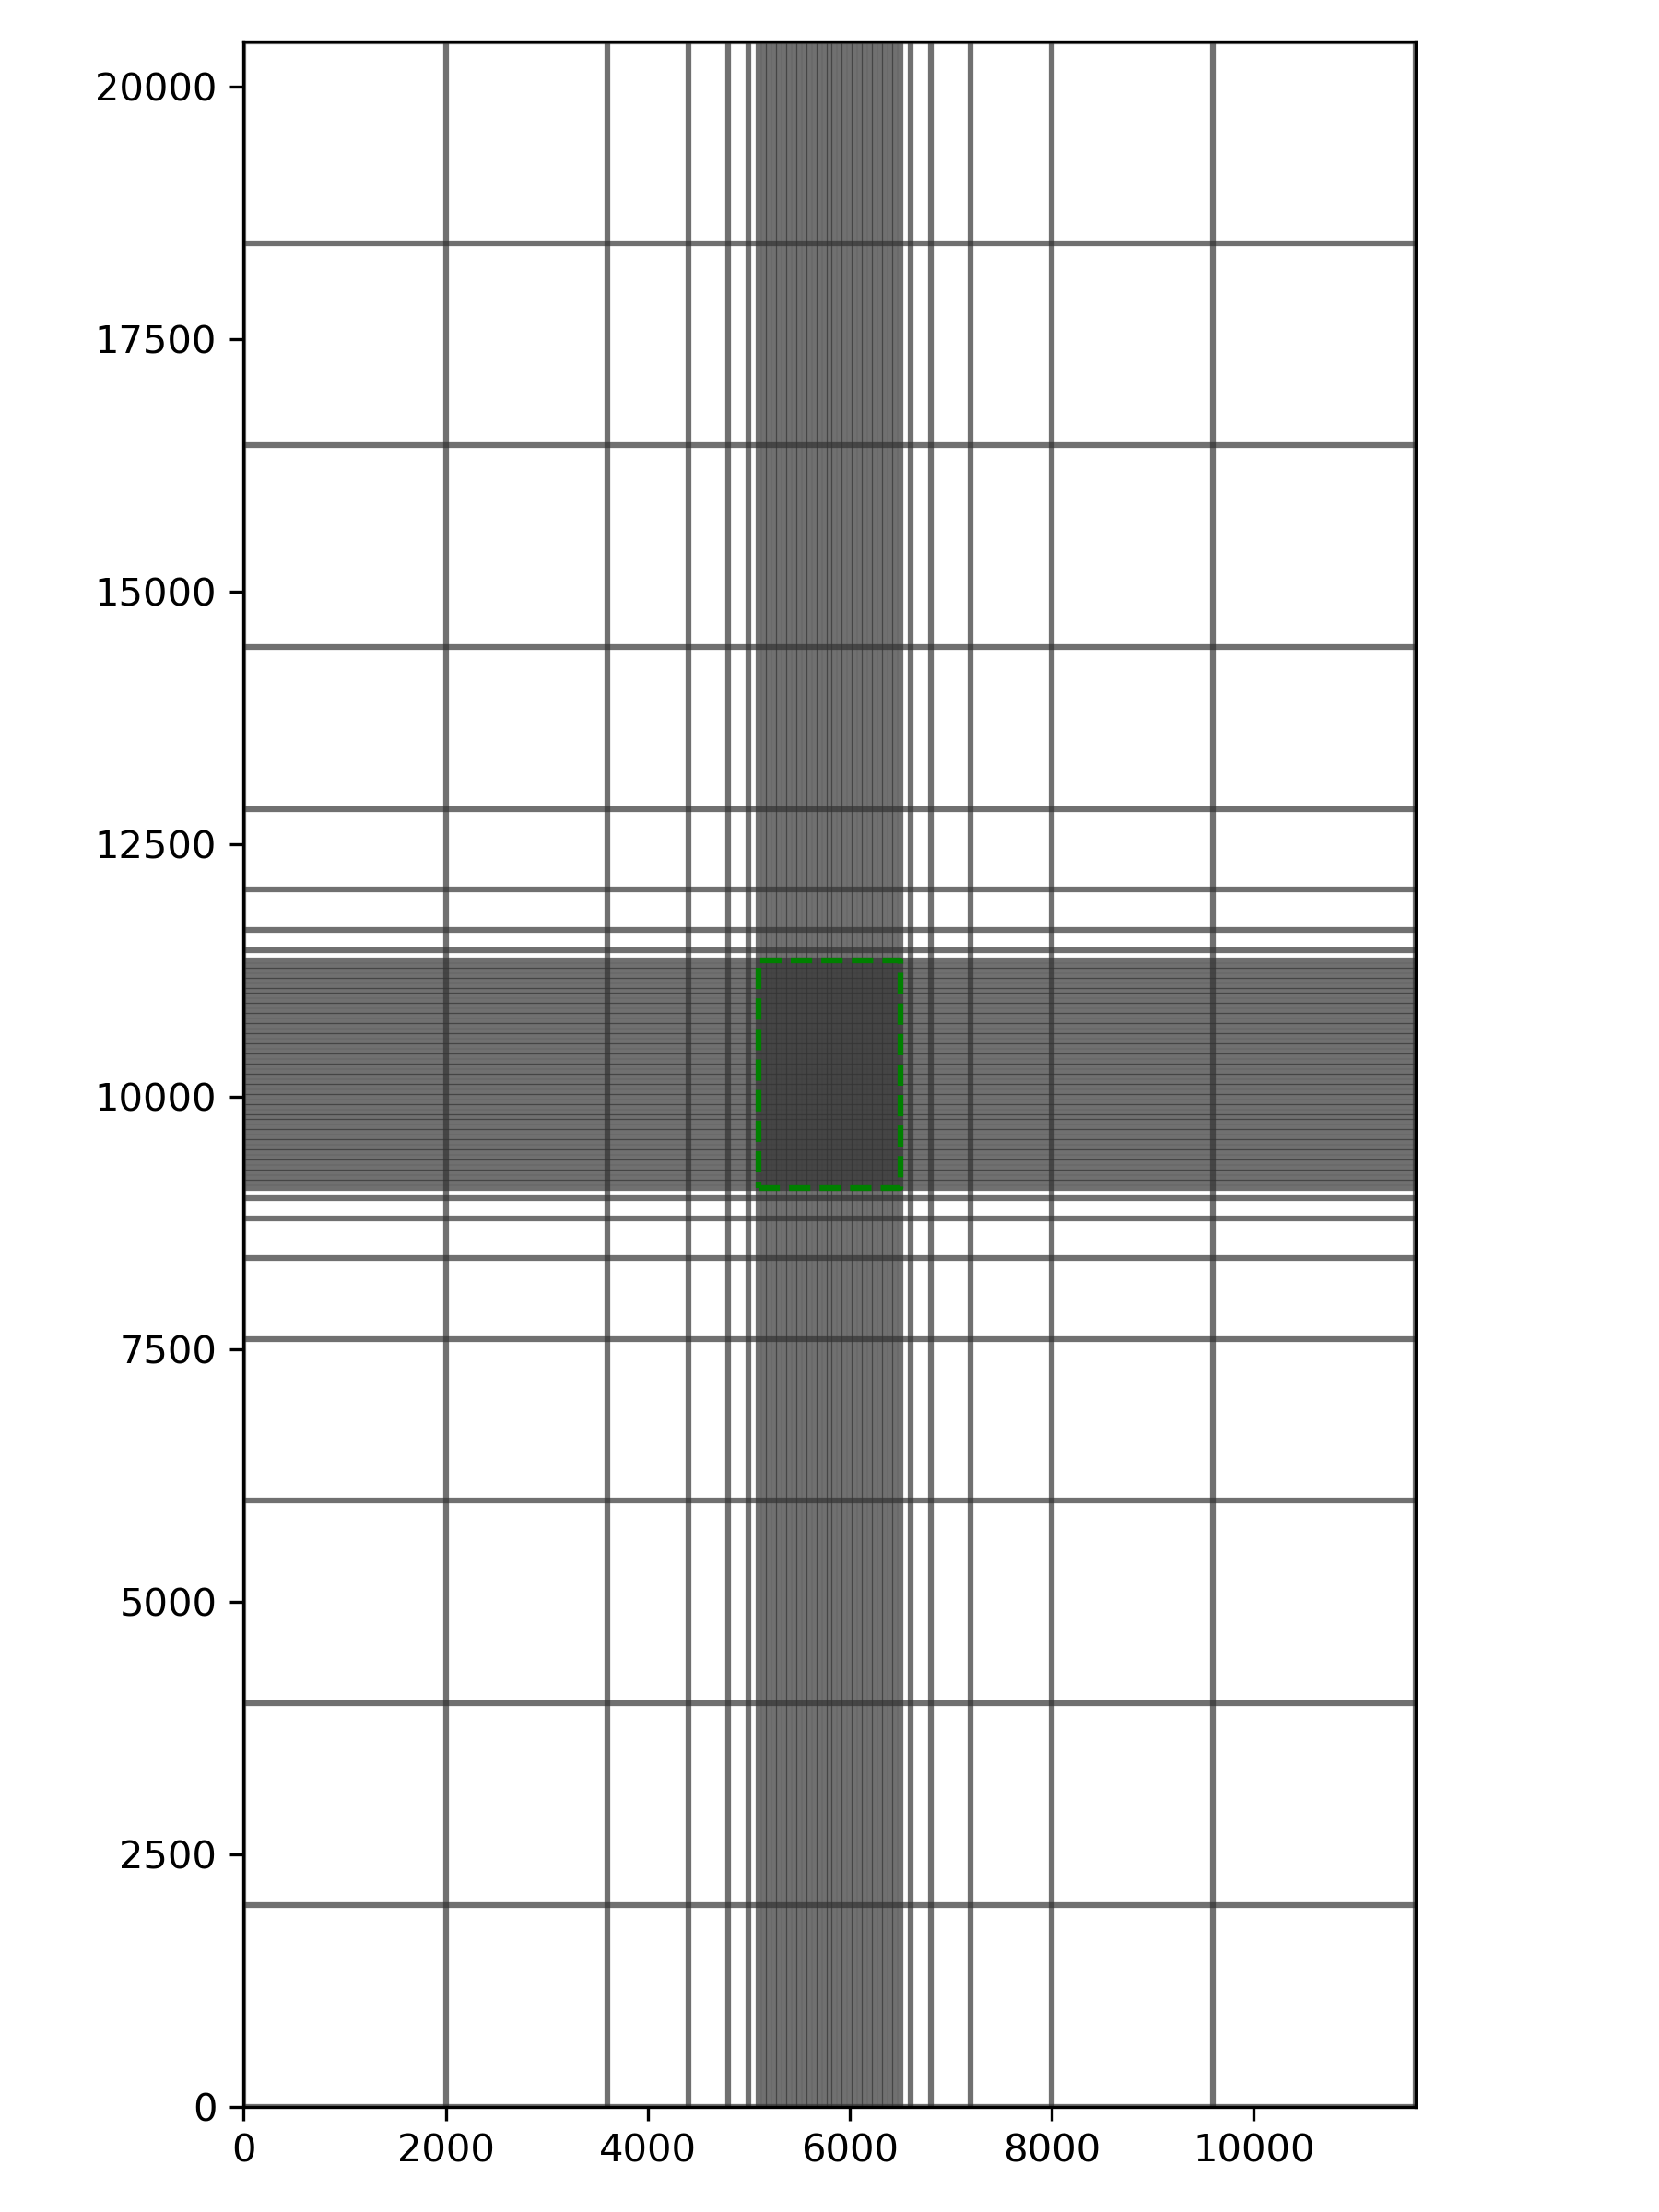
\includegraphics[width=0.5\textwidth]{./Figures/InterfaceModel/mt3dms-p10-modelgrid.png}
	\caption[A plan view of the model grid from MT3DMS problem 10]{A plan view of the model grid for the simulation as defined in MT3DMS problem 10. The green dashed rectangle shows the location of the interface that is used for decomposing this case into a system of coupled GWF and GWT models}
	\label{fig:gwtgwt-fullgrid}
	\end{center}
\end{figure}

To illustrate the concept of this new coupling, a well known, single-model case study (problem 10 in the MT3DMS manual \cite{zheng1999mt3dms}) is implemented as a coupled system where the connection between the GWT models is handled by the Interface Model framework. This study is part of the official set of examples that comes with every \mf software release\footnote{https://modflow6-examples.readthedocs.io/en/master/}. The coefficients for the flow coupling in this case are calculated with the basic GWF Model Exchange module and the following discussion will focus on the GWT-GWT exchange. Figure~\ref{fig:gwtgwt-fullgrid} shows a plan view of the grid and the location of the interface between the submodels. Note that changing only the composition of the grid and leaving the model configuration the same, does not affect the outcome of the simulation\footnote{At the highest level of detail, the outcome does change because the numbering of the grid nodes is different in both scenarios leading to a reordered matrix system to be solved. As expected, these differences turn out to be well within the configured (IMS) solver tolerance.} and therefore makes for a very suitable test case of this coupling.

\begin{figure}[!ht]
	\begin{center}
	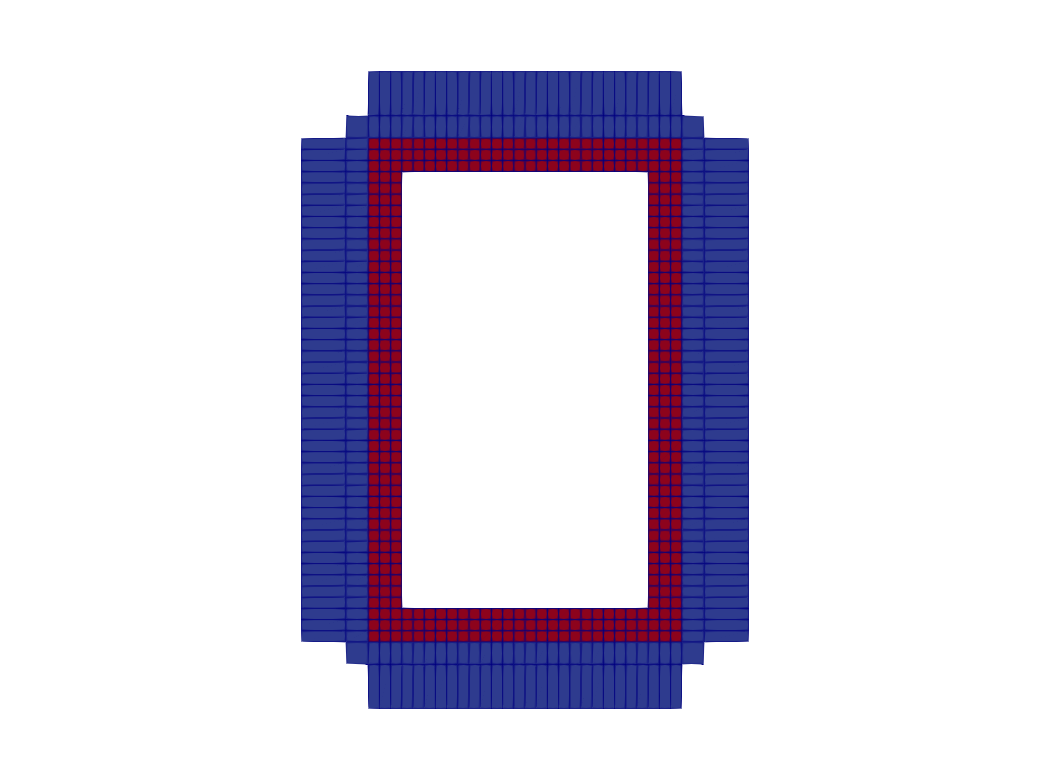
\includegraphics[width=0.8\textwidth]{./Figures/InterfaceModel/gwt-ifmod-grid.png}
	\caption[A top view of the Interface Model grid]{A top view of the grid for the Interface Model belonging to the inner GWT model in the example described in the text. The blue cells are located in the outer model’s grid, the red cells are internal. Note that deeper layers have an identical horizontal structure.}
	\label{fig:gwtgwt-interface-grid}
	\end{center}
\end{figure}

Figure~\ref{fig:gwtgwt-interface-grid} shows a plan view of the grid that is reconstructed as part of the Interface Model for the inner GWT model. The red band with cells belong to the inner model’s grid and the blue cells are part of the outer, coarser grid. Because two Interface Models are constructed for every Exchange, (one for each of the models in it) a similar though not identical picture can be drawn for the outer GWT model. However, the extent of this grid is not necessarily equal on both sides of the exchange. The task of the Interface Model is twofold. First of all, it is designed to calculate the coefficients for the linear system for fluxes through the faces directly at the interface. Additionally, it can provide coefficients for those fluxes that would be affected by cells on the other side of the interface just as if the simulation would have been set up as a single model. It is the requirement to support the latter that causes the asymmetry. This becomes clearer when looking at Figure~\ref{fig:gwtgwt-stencils} which shows the XT3D computational stencils and how they determine what the required extent of the interface grid is. To determine the flux through a face at the model interface, the cells on either side and their immediate neighbors are sufficient (the circle). To correctly calculate the flux through cell faces not directly at the interface but influenced by the connection to another model, more additional levels of connectivity are required, depending on the exact size of the computation stencil (the diamond).

\begin{figure}[!ht]
	\begin{center}
	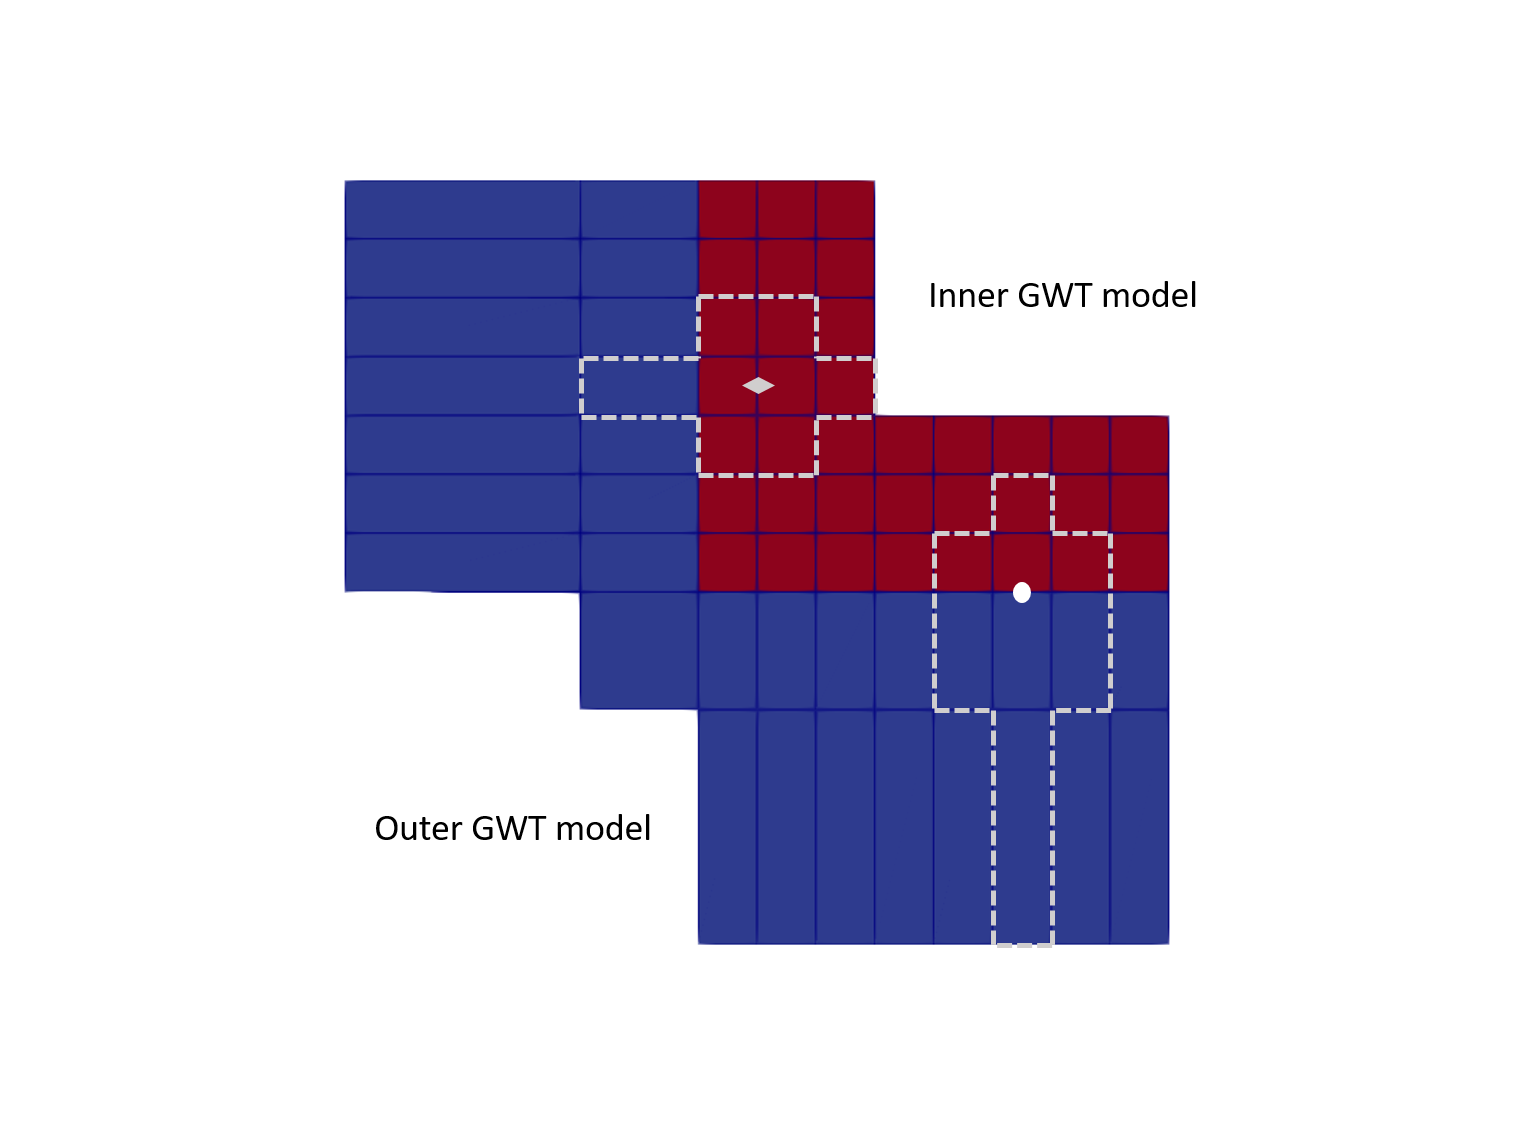
\includegraphics[width=0.8\textwidth]{./Figures/InterfaceModel/gwt-ifmod-stencils.png}
	\caption[Stencil size and the extent of the Interface Model grid]{Top view when zoomed in to the South-West corner of the interface grid. The dashed line surrounds the grid cells participating in the calculation of the dispersive XT3D flux directly at the interface (the white circle) and through a face in the model’s interior (the white diamond) which is nonetheless affected by the connection to the outer GWT model. The extension of the computational stencil in the vertical direction is omitted but straightforward.}
	\label{fig:gwtgwt-stencils}
	\end{center}
\end{figure}

This case study is used to demonstrate the concept of the generalized coupling method with the Interface Model. It serves as an excellent test case because the outcome should be identical to the known results, at least within the configured tolerance of the Numerical Solution. However, from a modeling perspective it would make more sense to redesign the model grid of the problem. With the new capability to use the multi-model approach also for problems containing solute transport, there is no longer a need to refine the study area by using varying column and row width as was done in the original MT3DMS problem. Both the study area and the surrounding domain can be configured as coupled models with a regularly structured (DIS) grid. The granularity of the inner grid can be independently refined to improve the resolution of the results without the need to set up the entire problem based on an unstructured (DISU) grid.

Finally, such a setup would allow to apply the Interface Model in another powerful way. A refinement of the grid is known to produce inaccuracies at the interface, as discussed in the introduction of \cite{modflow6xt3d}. This can be remedied by enabling the XT3D option in the GWF NPF package. The new coupling mechanism based on the Interface Model makes it now possible to enable this option \emph{only} at the interface, which will mitigate the distorting effects of such a grid refiniment on the calculated flow field and still avoids the computational overhead of calculating the XT3D terms on the entire domain.



\newpage
\incchap
\SECTION{Chapter \thechapno. Accounting for Fluid Viscosity}
\customlabel{ch:vscpackage}{\thechapno}

The dynamic viscosity of a fluid is a function of fluid composition and temperature and typically has a weak dependence on pressure. In some applications, particularly those that involve large variations in temperature, viscosity can vary significantly in space and over time. Variations in viscosity, in turn, can affect groundwater flow by changing the hydraulic conductivity, which is inversely proportional to viscosity. In the original release of \mf, variations in viscosity and their effects on hydraulic conductivity were not taken into account. The \mf Viscosity (VSC) Package allows viscosity to vary as a function of solute concentrations and fluid temperature and accounts for the effect of variable viscosity on hydraulic conductivity in the Node-Property Flow (NPF) Package and in stress packages that involve head-dependent groundwater flow. Temperature-dependent viscosity has been implemented in other groundwater modeling codes, including HST3D \citep{kipp1987}, VS2DH \citep{healy1996}, SUTRA-MS \citep{hughes2004}, and SEAWAT Version 4 \citep{langevin2008seawat}. Like these other codes, the VSC Package does not account for the dependence of viscosity on pressure, which is negligible in most applications.

For cases in which the rate of groundwater flow is proportional to the head gradient in the direction of flow, as in an isotropic porous medium, the flow between two adjacent locations can be approximated using a one-dimensional form of Darcy's Law \citep[equation 4-15]{modflow6gwf}:

\begin{equation}
\label{eqn:modflow6gwf-4-15}
Q = C \left( h_{1} - h_{2} \right),
\end{equation}

\noindent where $h_{1}$ and $h_{2}$ are the hydraulic heads at locations 1 and 2, respectively, $Q$ is the flow from location 1 to location 2, and $C$ is a hydraulic conductance defined by~\citep[equation 4-14]{modflow6gwf}:

\begin{equation}
\label{eqn:modflowgwf-4-14}
C = \frac{K A} {L_{1,2}},
\end{equation}

\noindent where $K$ is the hydraulic conductivity of the porous medium that connects the two locations, $A$ is the cross-sectional area perpendicular to flow, and $L_{1,2}$ is the distance between two locations. A form of equation~\ref{eqn:modflow6gwf-4-15} is used in the \mf ``conductance-based'' formulation for flow between two adjacent model cells \citep{modflow6gwf}. In that case, the conductance is based on an effective hydraulic conductivity between the two cells, the area of the cell-cell interface, and the distance between the cell centers. A form of equation~\ref{eqn:modflow6gwf-4-15} is also used in \mf stress packages in which the flow into or out of the model at a model boundary is head-dependent. For example, in the General-Head Boundary (GHB) Package, flow between an external source and a groundwater model cell is proportional to the difference between the head assigned to the external source and the simulated head in the cell, and the conductance is representative of the material between the external source and the cell center.

Because hydraulic conductivity is inversely proportional to viscosity, the conductivity $K$ for a simulated fluid composition and temperature is related to the conductivity $K_{0}$ for some reference composition and temperature by

\begin{equation}
\label{eqn:conductivity-ratio}
K = \frac{\mu_{0}}{\mu} K_{0}.
\end{equation}

\noindent It follows from equation~\ref{eqn:modflowgwf-4-14} that the conductance $C$ for a simulated fluid composition and temperature is related to the conductance $C_{0}$ for the reference composition and temperature by

\begin{equation}
\label{eqn:conductance-ratio}
C = \frac{\mu_{0}}{\mu} C_{0},
\end{equation}

\noindent where $\mu$ and $\mu_{0}$ are the viscosities at the simulated and reference conditions, respectively. The VSC Package uses equations~\ref{eqn:conductivity-ratio} and~\ref{eqn:conductance-ratio} to update hydraulic conductivities and conductances to account for changes in solute concentrations and temperature during a flow and transport simulation based on the Groundwater Flow (GWF) and Groundwater Transport (GWT) Models. The GWT Model is designed to simulate solute transport but can be used to simulate heat transport in some applications by appropriately scaling the input parameters to render the solute-transport equation mathematically equivalent to the heat-transport equation \citep{zheng2010supplemental}. In such cases, the ``solute concentration'' calculated by a GWT-based heat-transport model can by identified in the VSC Package input file as representing temperature. Although the VSC Package allows viscosity to vary with solute concentration, variations in viscosity are typically most significant in heat-transport applications.

\subsection{Dependence of Viscosity on Concentration and Temperature} \label{sec:fluidvsc}

The VSC Package calculates viscosity as a function of concentration and temperature using the following equation \citep[equation 17]{langevin2008seawat}:

\begin{equation}
\label{eqn:viscfunc}
\mu = \mu_T \left ( T \right ) + \sum_{k=1}^{NS} \frac{\partial \mu} {\partial C^k} \left ( C^k - C_{0}^k \right ) 
\end{equation}

\noindent where $NS$ is the number of chemical species (solutes) whose concentrations affect viscosity, $C^k$ and $C_{0}^k$ are the simulated and user-specified reference concentrations of species $k$, respectively, and $\partial \mu / \partial C^k$ is the user-specified rate at which viscosity changes linearly with the concentration of species $k$. (Symbols $C^k$ and $C_{0}^k$ are not to be confused with the symbols for conducance, $C$ and $C_0$, introduced earlier.) When all concentrations are equal to their reference values, the viscosity is equal to $\mu_T \left ( T \right )$, which embodies the dependence of viscosity on temperature according to

\begin{align}
	\label{eqn:viscT}
	 \mu_T \left ( T \right ) = \begin{dcases}
		\mu_{0} + \frac{\partial \mu} {\partial T} \left ( T - T_{0}\right ) & linear \\
		\mu_{0} A_2^{\frac{A_3 \left ( T_0 - T \right )} {\left ( T + A_4 \right ) \left ( T_0 + A_4 \right ) }} & nonlinear
	\end{dcases} .
\end{align}

\noindent where $T$ and $T_{0}$ are the simulated and user-specified reference temperature, respectively, and $\mu_{0}$ is the user-specified reference viscosity. The reference viscosity is commonly set to 0.001 kg~m$^{-1}$~s$^{-1}$, which is representative of freshwater at a reference temperature of 20$^{\circ}$C \citep[Table 11.1]{maidment1993}. When $T$ equals $T_{0}$, or if temperature is not designated by the user as affecting viscosity, $\mu_T \left ( T \right )$ equals $\mu_{0}$. Equation~\ref{eqn:viscT} includes both linear and nonlinear variation of viscosity with temperature. Linear variation is the default, in which case $\partial \mu / \partial T$ is the user-specified rate at which viscosity changes linearly with temperature. Nonlinear variation is a user-selectable option, in which case the variation of viscosity from the reference value is determined by user-specified parameters $A_2$, $A_3$, and $A_4$. The nonlinear option in equation~\ref{eqn:viscT} is mathematically equivalent to one of the options available in SEAWAT Version 4 \citep[equation 18]{langevin2002seawat} but is written in a form that explicitly sets $\mu_T \left ( T \right )$ equal to $\mu_{0}$ when $T$ equals $T_{0}$. Setting $\mu_0$, $A_2$, $A_3$, and $A_4$ to 0.001002 kg~m$^{-1}$~s$^{-1}$, 10.0, 248.37, and 133.15, respectively, and rounding the lead coefficient to one decimal place gives the temperature dependence of viscosity used in SUTRA \citep{voss1984sutra} and SUTRA-MS \citep{hughes2004}. VS2DH \citep{healy1996} also calculate the temperature dependence of viscosity using functions that are, respectively, mathematically equivalent to and a special case of equation~\ref{eqn:viscT}.

Over the temperature range $0-40^{\circ}$C, the viscosity of freshwater varies between approximately 0.0007 and 0.00175 kg~m$^{-1}$~s$^{-1}$, as indicated by the nonlinear (blue) curve in figure~\ref{fig:viscosityrelation}. The black line in figure~\ref{fig:viscosityrelation} depicts a linear approximation that coincides with the nonlinear curve at the reference temperature and viscosity, $\left ( T_0, \mu_0 \right ) = \left(\right.$20$^{\circ}$C, 0.001 kg~m$^{-1}$~s$^{-1}\left.\right)$.

\begin{figure}
	\begin{center}
	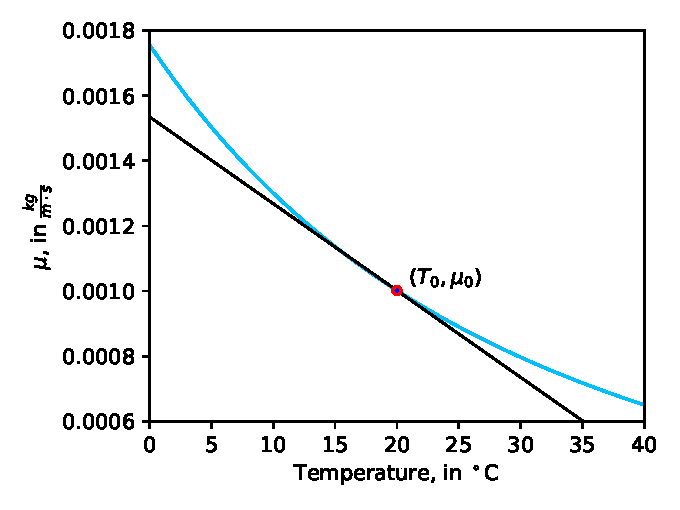
\includegraphics{./Figures/VSCnonlinear.pdf}
	\caption[Graph showing the nonlinear response in the viscosity as temperature changes]{Nonlinear dependence of viscosity on temperature (blue curve) that is representative of freshwater over the temperature range $0-40^{\circ}$C, and a linear approximation (black curve) that has the same value $\left ( \mu_0 \right )$ and slope at the reference temperature $\left ( T_0 \right )$.  The blue curve is generated using 0.001002 kg~m$^{-1}$~s$^{-1}$,10.0, 248.37, and 133.15 for $\mu_0$, $A_2$, $A_3$, and $A_4$, respectively}
	\label{fig:viscosityrelation}
	\end{center}
\end{figure}

\subsection{Accounting for Variable Viscosity in Flows Between Cells} \label{sec:gwfvsc}

The VSC Package uses concentrations and temperatures calculated for each cell by a GWT model on the previous time step or outer solution iteration to calculate viscosities for the current time step. These viscosities are used to adjust cell hydraulic conductivity values in the NPF Package using equation~\ref{eqn:conductivity-ratio}. The reference values of conductivity are the values specified by the user in the NPF Package and, optionally, the Time-Varying Conductivity (TVK) Package (Chapter 6 of this document). The conductivity adjustment is performed after the user-specified conductivities are read in but before conductivity values are passed to program units that use cell conductivities to formulate expressions for flow between cells, which include the ``conductance-based'' formulation for flow and the XT3D capability \citep{modflow6xt3d}. If the VSC Package is not active, cell conductivities are not adjusted for variable viscosity, and the user-specified values are used.

\subsection{Accounting for Variable Viscosity in Boundary Flows} \label{sec:gwfvsc}

The VSC Package uses concentrations and temperatures calculated for each cell by a GWT model on the previous time step or outer solution iteration in calculating viscosities for the current time step. These viscosities are used to adjust hydraulic conductances, using equation~\ref{eqn:conductance-ratio}, in stress packages that involve head-dependent boundary flows, which include the River (RIV), General-Head Boundary (GHB), Drain (DRN), Streamflow Routing (SFR), Lake (LAK), and Multi-Aquifer Well (MAW) Packages \citep{modflow6gwf}. For a boundary flow out of the model, the viscosity is based on the simulated concentration or temperature in the cell from which the boundary flow originates. For a boundary flow into the model, the viscosity is based on the concentration or temperature of the water entering the cell from the boundary. The reference values of conductance are the values normally set or calculated by the stress package based on user input. The conductance adjustment is performed after the stress package completes its normal conductance calculation but before the conductance value is used to formulate the expression for the boundary flow. If the VSC Package is not active, stress-package conductances are not adjusted for variable viscosity.



\newpage
\incchap
\SECTION{Chapter \thechapno. Revised Parameterization of Transport for Combined Mobile and Immobile Domain Simulations}
\customlabel{ch:sorption}{\thechapno}

The Groundwater Transport (GWT) Model \citep{modflow6gwt} in \mf can simulate a variety of solute-transport processes in aquifer material that includes ``mobile" and ``immobile" domains. The mobile and immobile domains are conceptualized as coexisting within a model cell and can exchange solute with each other. The mobile domain is always simulated by the GWT Model.  Transport in an immobile domain, which may be optionally defined by the user, is simulated by the Immobile Storage and Transfer (IST) Package \citep{modflow6gwt} for the GWT Model. Multiple instances of the IST Package may be invoked to represent multiple immobile domains.

In \mf version 6.4.2, the parameterization of the equations that govern transport in the mobile and immobile domains has been revised, and corresponding changes have been made to the input requirements for porosity, domain fraction, and bulk density. The revised parameterization is expected to be more intuitive for users in many mobile-immobile transport applications. It will also allow users to model a wider variety of solute transport scenarios involving immobile-domain sorption than the original parameterization used in versions of \mf up to and including version 6.4.1.

Input for existing \mf models that include one or more immobile domains can be converted from the original parameterization to the revised parameterization such that the simulated transport behavior remains the same. No changes to the model input are needed for existing \mf models that do not include an immobile domain.

The remainder of this chapter begins with a review of the original parameterization of transport described in \citep{modflow6gwt}. The revised parameterization is then presented, and guidance is provided for converting existing model input from the original parameterization to the revised parameterization.

\subsection{Review of the Original Parameterization} \label{sec:origparamreview}

With the original parameterization used in versions of \mf up to and including version 6.4.1, the partial differential equation that represents the conservation of solute mass at points in the mobile domain is equation 2--1 of \cite{modflow6gwt}, which is reproduced here as

\begin{equation}
\label{eqn:gwtpdeorig}
\begin{aligned}
\frac {\partial \left ( S_w \theta_m C \right )}{\partial t} = 
- \nabla \cdot \left ( \matr{q} C  \right ) 
+ \nabla \cdot \left ( S_w \theta_m \matr{D} \nabla C \right ) 
+ q'_s C_s + M_s  
- \lambda_1 \theta_m S_w C - \gamma_1 \theta_m S_w \\
- f_m \rho_b \frac {\partial \left ( S_w \overline{C} \right ) }{\partial t} 
- \lambda_2 f_m \rho_b S_w \overline{C} - \gamma_2 f_m \rho_b S_w 
- \sum \limits_{im=1}^{nim}  \zeta_{im} S_w \left ( C - C_{im} \right )
\end{aligned}
\end{equation}

\noindent where $S_w$ is the water saturation defined as the volume of water per volume of voids ($L^3/L^3$), $C$ is the mobile-domain volumetric concentration of solute expressed as mass of dissolved solute per unit volume of mobile-domain fluid ($M/L^3$), $t$ is time ($T$), $\matr{q}$ is the vector of specific discharge ($L/T$), $\matr{D}$ is the second-order tensor of hydrodynamic dispersion coefficients ($L^2/T$), $q'_s$ is the volumetric flow rate per unit volume of aquifer (defined as positive for flow into the aquifer) for mass sources and sinks ($1/T$), $C_s$ is the volumetric solute concentration of the source or sink fluid ($M/L^3$), $M_s$ is rate of solute mass loading per unit volume of aquifer ($M/L^3T$), $\lambda_1$ is the first-order decay rate coefficient for dissolved solute in the mobile domain ($1/T$), $\gamma_1$ is the zero-order decay rate coefficient for dissolved solute in the mobile domain ($M/L^3T$), $\overline{C}$ is the concentration of sorbate (sorbed solute) expressed as mass of sorbate per unit mass of solid aquifer material in the mobile domain ($M/M$), $\lambda_2$ is the first-order decay rate coefficient ($1/T$) for sorbate in the mobile domain, $\gamma_2$ is the zero-order decay rate coefficient ($M/MT$) for sorbate in the mobile domain, $nim$ is the number of immobile domains, $\zeta_{im}$ is the rate coefficient for the transfer of mass between the mobile domain and immobile domain $im$ ($1/T$), $C_{im}$ is an immobile-domain volumetric concentration of solute expressed as mass of dissolved solute per unit volume of fluid in immobile domain $im$ ($M/L^3$), $\rho_{b}$ is the bulk density of the aquifer material defined as the mass of solid aquifer material per unit volume of aquifer ($M/L^3$), $\theta_m$ is the mobile-domain effective porosity defined as defined as volume of voids participating in mobile-domain transport per unit volume of aquifer ($L^3/L^3$), and $f_m$ is the fraction of the mass of aquifer solid material that is in the mobile domain ($M/M$). To avoid potential confusion with the total porosity, in equation~\ref{eqn:gwtpdeorig} the mobile porosity is intentionally given the symbol $\theta_m$, which is different than the symbol $\theta$ used by \cite{modflow6gwt}. Also, note that \cite{modflow6gwt} define $f_m$ as ``the fraction of aquifer solid material available for sorptive exchange with the mobile phase under fully saturated conditions," which is correct only if all the aquifer solid material in the mobile domain is available for sorptive exchange and the fraction is understood to be a mass fraction.

The Immobile Storage and Transfer (IST) Package for the GWT Model allows users to designate a fraction of a model cell as immobile. With the original parameterization used in versions of \mf up to and including version 6.4.1, the partial differential equation that represents the conservation of solute mass at points in an immobile domain is equation 7--2 of \cite{modflow6gwt}, which is reproduced here as 

\begin{equation}
\label{eqn:gwtistpdeorig}
\begin{split}
\theta_{im} \frac{\partial C_{im} }{\partial t} + f_{im} \rho_b \frac{\partial \overline{C}_{im}}{\partial t} = 
- \lambda_{1,im} \theta_{im} C_{im} - \lambda_{2,im}  f_{im} \rho_b \overline{C}_{im} \\
- \gamma_{1,im} \theta_{im} - \gamma_{2,im} f_{im}  \rho_b 
+ \zeta_{im} S_w \left ( C - C_{im} \right ),
\end{split}
\end{equation}

\noindent where $\overline{C}_{im}$ is the concentration of sorbate (sorbed solute) expressed as mass of sorbate per unit mass of solid aquifer material in the immobile domain ($M/M$), $\lambda_{1,im}$ is the first-order reaction rate coefficient for dissolved solute in the immobile domain ($1/T$), $\lambda_{2,im}$ is the first-order reaction rate coefficient for sorbate in the immobile domain ($1/T$), $\gamma_{1,im}$ is the zero-order reaction rate coefficient for dissolved solute in the immobile domain ($ML^{-3}T^{-1}$), $\gamma_{2,im}$ is the zero-order reaction rate coefficient for sorbate in the immobile domain ($M M^{-1}T^{-1}$), $\theta_{im}$ is the effective porosity in the immobile domain defined as volume of voids participating in immobile-domain transport per unit volume of immobile domain $im$ ($L^3/L^3$), and $f_{im}$ is the fraction of the mass of aquifer solid material that is in immobile domain $im$ ($M/M$). Note that \cite{modflow6gwt} define $f_{im}$ as ``the fraction of aquifer solid material available for sorptive exchange with the immobile domain under fully saturated conditions," which is correct only if all the aquifer solid material in the immobile domain is available for sorptive exchange and the fraction is understood to be a mass fraction.

The original model parameters that are affected by the revised parameterization are listed in table~\ref{table:origparam}. Note that in the original parameterization, division of the aquifer into mobile and immobile domains is conceptualized in terms solid mass fractions, and porosities and bulk densities are defined on a per-aquifer-volume basis. Note also that the user is required (in versions of \mf up to and including version 6.4.1) to provide the value of the overall bulk density, $\rho_b$, in the input for each package that represents a domain in which sorption is active (the MST Package for the mobile domain, and the IST Package for immobile domains).

\begin{table}[!ht]
  \small
  \centering
  \caption{Symbols, descriptions, and definitions of original mobile and immobile domain model parameters (used in versions of \mf up to and including version 6.4.1) that are affected by the revised parameterization. In the original parameterization, division of the aquifer into domains is conceptualized in terms of solid mass fractions, and domain properties are defined on a per-aquifer-volume basis} \tabularnewline 

  \begin{tabular}{z{1.50cm}
                  z{3.50cm}
                  z{5.00cm}
                  z{3.50cm}
                  }
    % header
    \hline
    \rowcolor{Gray}
    \multicolumn{1}{ z{1.50cm} }{\textbf{Symbol}} & 
    \multicolumn{1}{ z{3.50cm} }{\textbf{Description}} & 
    \multicolumn{1}{ z{5.00cm} }{\textbf{Definition}} &
    \multicolumn{1}{ z{3.50cm} }{\textbf{Notes}} \\
    \hline

    $\theta_m$ &  porosity (mobile domain) &  $\frac{mobile \; domain \; pore \; volume}{aquifer \; volume}$ & sorption-related input parameter \\
    
\rowcolor{Gray}
    $\theta_{im}$ &  porosity (immobile domain $im$) &  $\frac{immobile \; domain \; pore \; volume}{aquifer \; volume}$ & sorption-related input parameter \\

    $\rho_{b}$ & overall bulk density (mobile and immobile domains combined) &  $\frac{aquifer \; solid \; mass}{aquifer \; volume}$ & sorption-related input parameter \\

\rowcolor{Gray}
    $f_{m}$ &  solid mass fraction (mobile domain) &  $\frac{mobile \; domain \; solid \; mass}{aquifer \; solid \; mass}$ & sorption-related parameter (not input; calculated by \mf from immobile-domain solid mass fractions) \\

    $f_{im}$ &  solid mass fraction (immobile domain $im$) &  $\frac{immobile \; domain \; solid \; mass}{aquifer \; solid \; mass}$ & sorption-related parameter (not input; calculated by \mf from user-specified domain porosities) \\
    
    \hline
  \end{tabular}
  \label{table:origparam}
\end{table}


Immobile-domain solid mass fractions, $f_{im}$, are not input by the user; rather, they are calculated by \mf (in versions up to and including 6.4.1) from user-input porosities using

\begin{equation}
\label{eqn:fim1}
f_{im} = \frac{\theta_{im}}{\theta_t}.
\end{equation}

\noindent where $\theta_t$ is the total porosity [which is erroneously represented by the symbol $\theta$ in the related text on p. 7--2 of \cite{modflow6gwt}]. The mobile-domain solid mass fraction is then calculated by \mf (in versions up to and including 6.4.1) using

\begin{equation}
\label{eqn:fm0}
f_m = 1 - \sum_{im}f_{im},
\end{equation}

\noindent where the summation is over all immobile domains specified by the user. Equations~\ref{eqn:fm0} and~\ref{eqn:fim1}, together with the definition of total porosity,

\begin{equation}
\label{eqn:thetat1}
\theta_t = \theta_m + \sum_{im}{\theta_{im}},
\end{equation}

\noindent imply that the default value of the mobile domain solid mass fraction is given by

\begin{equation}
\label{eqn:fm1}
f_m = 1 - \sum_{im}f_{im} = 1 - \frac{\sum_{im}\theta_{im}}{\theta_t} = \frac{\theta_m}{\theta_t}.
\end{equation}

\noindent If there are no immobile domains, the total porosity is the same as the mobile porosity and $f_m$ is 1.

\subsection{Revised Parameterization} \label{sec:revisedparam}

The revised parameterization described in this chapter differs from the original parameterization, which is described in \cite{modflow6gwt} and summarized above, in the following ways:

\begin{itemize}
\item Two sets of parameter substitutions are implemented in governing equations~\ref{eqn:gwtpdeorig} and~\ref{eqn:gwtistpdeorig}. These substitutions recast the model input in terms of parameters that are expected be more intuitive for users in many applications.
  \begin{itemize}
  \item Domain porosities $\theta_{m}$ and $\theta_{im}$, which are defined on a per-aquifer-volume basis, are replaced by the mathematically equivalent expressions $\hat{f}_{m} \phi_{m}$ and $\hat{f}_{im} \phi_{im}$, respectively, where $\hat{f}_{m}$ and $\hat{f}_{im}$ are domain volume fractions (instead of mass fractions) and $\phi_{m}$ and $\phi_{im}$ are domain porosities defined on a per-domain-volume basis.
  \item The parameter products $f_{m} \rho_{b}$ and $f_{im} \rho_{b}$ are replaced by the mathematically equivalent products $\hat{f}_{m} \rho_{b, m}$ and $\hat{f}_{im} \rho_{b, im}$, respectively, where $\rho_{b, m}$ and $\rho_{b, im}$ are domain bulk densities defined on a per-domain-volume basis.
  \end{itemize}
\item Unlike the domain mass fractions $f_{m}$ and $f_{im}$, which are set automatically by \mf (in versions up to and including 6.4.1) based on domain porosities in the original parameterization, the domain volume fractions $\hat{f}_{m}$ and $\hat{f}_{im}$ are specified directly by the user in the revised parameterization, offering the flexibility to accurately characterize sorption in a wider variety of mobile-immobile systems.
\end{itemize}

With the changes to the parameterization summarized above, the partial differential equations that represent the conservation of solute mass at points in the mobile and immobile domains can be written as

\begin{equation}
\label{eqn:gwtpde}
\begin{aligned}
\frac {\partial \left ( S_w \theta_m C \right )}{\partial t} = 
- \nabla \cdot \left ( \matr{q} C  \right ) 
+ \nabla \cdot \left ( S_w \theta_m \matr{D} \nabla C \right ) 
+ q'_s C_s + M_s  
- \lambda_1 \theta_m S_w C - \gamma_1 \theta_m S_w \\
- \hat{f}_m \rho_{b,m} \frac {\partial \left ( S_w \overline{C} \right ) }{\partial t} 
- \lambda_2 \hat{f}_m \rho_{b,m} S_w \overline{C} - \gamma_2 \hat{f}_m \rho_{b,m} S_w 
- \sum \limits_{im=1}^{nim}  \zeta_{im} S_w \left ( C - C_{im} \right )
\end{aligned}
\end{equation}

\noindent where

\begin{equation}
\label{eqn:thetam_from_revparams}
\theta_{m} = \hat{f}_{m} \phi_{m} ,
\end{equation}

\noindent and

\begin{equation}
\label{eqn:gwtistpde}
\begin{split}
\theta_{im} \frac{\partial C_{im} }{\partial t} + \hat{f}_{im} \rho_{b,im} \frac{\partial \overline{C}_{im}}{\partial t} = 
- \lambda_{1,im} \theta_{im} C_{im} - \lambda_{2,im}  \hat{f}_{im} \rho_{b,im} \overline{C}_{im} \\
- \gamma_{1,im} \theta_{im} - \gamma_{2,im} \hat{f}_{im} \rho_{b,im} 
+ \zeta_{im} S_w \left ( C - C_{im} \right ),
\end{split}
\end{equation}

\noindent where

\begin{equation}
\label{eqn:thetaim_from_revparams}
\theta_{im} = \hat{f}_{im} \phi_{im} .
\end{equation}

\noindent respectively. Model parameters and variables in equations~\ref{eqn:gwtpde} and ~\ref{eqn:gwtistpde} are defined as in equations~\ref{eqn:gwtpdeorig} and ~\ref{eqn:gwtistpdeorig}, except for the new parameters introduced in the revised parameterization: $\hat{f}_m$ is the volume fraction of the mobile domain defined as the volume of mobile domain per volume of aquifer ($L^3/L^3$), $\hat{f}_{im}$ is the volume fraction of the immobile domain defined as the volume of mobile domain $im$ per volume of aquifer ($L^3/L^3$), $\rho_{b,m}$ is the bulk density of aquifer material in the mobile domain defined as mass of solid aquifer material per unit volume of mobile domain ($M/L^3$), $\rho_{b,im}$ is the bulk density of aquifer material in the immobile domain defined as mass of solid aquifer material per unit volume of immobile domain $im$ ($M/L^3$), $\phi_m$ is the mobile-domain effective porosity defined as defined as volume of voids participating in mobile-domain transport per unit volume of mobile domain ($L^3/L^3$), and $\phi_{im}$ is the effective porosity in the immobile domain defined as defined as volume of voids participating in immobile-domain transport per unit volume of mobile domain $im$ ($L^3/L^3$). In the \mf code, porosities $\theta_{m}$ and $\theta_{im}$ are calculated from the new input parameters using equations~\ref{eqn:thetam_from_revparams} and ~\ref{eqn:thetaim_from_revparams} before being incorporated into discretized representations of equations~\ref{eqn:gwtpde} and~\ref{eqn:gwtistpde}. The new parameters are discussed in more detail below.

\subsubsection{Revised Parameters}

The new parameters are summarized in table~\ref{table:revparam}. Note that in  the revised parameterization, division of the aquifer into mobile and immobile domains is conceptualized in terms of volume fractions, and porosities and bulk densities are defined on a per-domain-volume basis. When an aquifer can be divided into multiple domains that occupy distinct, well-defined volumes, as when the mobile and immobile domains represent different lithologies, it may be intuitive to think in terms of the domain volume fractions and local domain properties (properties defined on a per-domain-volume basis).

\begin{table}[!ht]
  \small
  \centering
  \caption{Symbols, descriptions, and definitions of revised mobile and immobile domain model parameters introduced in \mf version 6.4.2. In the revised parameterization, division of the aquifer into domains is conceptualized in terms of volume fractions, and domain properties are defined on a per-domain-volume basis} \tabularnewline 

  \begin{tabular}{z{1.50cm}
                  z{3.50cm}
                  z{5.00cm}
                  z{3.50cm}
                  }
    % header
    \hline
    \rowcolor{Gray}
    \multicolumn{1}{ z{1.50cm} }{\textbf{Symbol}} & 
    \multicolumn{1}{ z{3.50cm} }{\textbf{Description}} & 
    \multicolumn{1}{ z{5.00cm} }{\textbf{Definition}} &
    \multicolumn{1}{ z{3.50cm} }{\textbf{Notes}} \\
    \hline

    $\phi_m$ &  porosity (mobile domain) &  $\frac{mobile \; domain \; pore \; volume}{mobile \; domain \; volume}$ & transport input parameter (not directly related to sorption) \\
    
\rowcolor{Gray}
    $\phi_{im}$ &  porosity (immobile domain $im$) &  $\frac{immobile \; domain \; pore \; volume}{immobile \; domain \; volume}$ & transport input parameter (not directly related to sorption) \\

    $\rho_{b,m}$ & bulk density (mobile domain) &  $\frac{mobile \; domain \; solid \; mass}{mobile \; domain \; volume}$ & sorption-related input parameter \\
    
\rowcolor{Gray}
    $\rho_{b,im}$ & bulk density (immobile domain $im$) &  $\frac{immobile \; domain \; solid \; mass}{immobile \; domain \; volume}$ & sorption-related input parameter \\

    $\hat{f}_{m}$ &  volume fraction (mobile domain) &  $\frac{mobile \; domain \; volume}{aquifer \; volume}$ & transport and sorption-related parameter (not input; calculated by \mf from immobile-domain volume fractions) \\

\rowcolor{Gray}
    $\hat{f}_{im}$ &  volume fraction (immobile domain $im$) &  $\frac{immobile \; domain \; volume}{aquifer \; volume}$ & transport and sorption-related input parameter \\

    \hline
  \end{tabular}
  \label{table:revparam}
\end{table}


\noindent All parameters in table~\ref{table:revparam} are model input parameters except the mobile-domain volume fraction, $\hat{f}_m$, which is calculated by \mf from the user-specified immobile-domain volume fractions using

\begin{equation}
\label{eqn:fm5}
\hat{f}_m = 1 -  \sum_{im}{\hat{f}_{im}},
\end{equation}

\noindent where the summation is over all immobile domains specified by the user. If there are no immobile domains,  $\hat{f}_m$ is set to 1.

Porosities and bulk densities in table~\ref{table:revparam} are defined on a per-domain-volume basis, i.e., as an amount per unit volume of domain. The total porosity, $\theta_t$, can be calculated as the volume-weighted average of the domain porosities, $\phi_m$ and $\phi_{im}$:

\begin{equation}
\label{eqn:thetat}
\theta_{t} = \theta_{m} + \sum_{im}{\theta_{im}} = \hat{f}_{m} \phi_{m} + \sum_{im}{\hat{f}_{im} \phi_{im}} ,
\end{equation}

\noindent Similarly, the overall bulk density, $\rho_b$, can be calculated as the volume-weighted average of the domain bulk densities, $\rho_{b, m}$ and $\rho_{b, im}$:

\begin{equation}
\label{eqn:rhob2}
\rho_{b} = \hat{f}_m \rho_{b, m} + \sum_{im}{\hat{f}_{im} \rho_{b, im}}.
\end{equation}

\subsection{Conversion of Existing Model Input to the Revised Parameterization} \label{sec:inputconversion}

Conversion of existing \mf model input to the revised parameterization such that the simulation gives the same numerical results requires that the revised mobile-domain solute conservation equation, equation~\ref{eqn:gwtpde}, be numerically equivalent to the original mobile-domain solute conservation equation, equation~\ref{eqn:gwtpdeorig}. This is achieved when $\hat{f}_{m}$ and $\phi_{m}$ satisfy

\begin{equation}
\label{eqn:equiv_porm}
\hat{f}_{m} \phi_{m} = \theta_{m}
\end{equation}

\noindent and, if sorption is active in the mobile domain, $\hat{f}_{m}$ and $\rho_{b, m}$ satisfy

\begin{equation}
\label{eqn:equiv_rhobm}
\hat{f}_{m} \rho_{b, m} = f_{m} \rho_{b} .
\end{equation}

\noindent For a model that includes at least one immobile domain, the revised immobile-domain solute conservation equation, equation~\ref{eqn:gwtistpde}, must also be numerically equivalent to the original immobile-domain solute conservation equation, equation~\ref{eqn:gwtistpdeorig}. This is achieved when $\hat{f}_{im}$ and $\phi_{im}$ satisfy

\begin{equation}
\label{eqn:equiv_porim}
\hat{f}_{im} \phi_{im} = \theta_{im}
\end{equation}

\noindent and, if sorption is active in immobile domain $im$, $\hat{f}_{im}$ and $\rho_{b, im}$ satisfy

\begin{equation}
\label{eqn:equiv_rhobim}
\hat{f}_{im} \rho_{b, im} = f_{im} \rho_{b} .
\end{equation}

\subsubsection{Simulation Without Immobile Domains}

For an existing simulation without immobile domains, which is the most common use case, no conversion of input parameters is needed to obtain the same simulation results. In this case, \mf sets $f_{m} = 1$ in the original parameterization and $\hat{f}_{m} = 1$ in the revised parameterization. Thus, equations~\ref{eqn:equiv_porm} and~\ref{eqn:equiv_rhobm} reduce to $\phi_{m} = \theta_{m}$ and $\rho_{b, m} = \rho_{b}$, respectively, and are satisfied by default by the original input values.

\subsubsection{Simulation With At Least One Immobile Domain}

For an existing simulation that includes at least one immobile domain, the values of the revised input parameters $\phi_{m}$, $\phi_{im}$, and $\hat{f}_{im}$ must be set such that they satisfy equations~\ref{eqn:equiv_porm} and~\ref{eqn:equiv_porim} in order to obtain the same simulation results. The value of $\hat{f}_{m}$ is calculated by \mf using equation~\ref{eqn:fm5}. Note that the immobile-domain fractions $\hat{f}_{im}$ must sum to less than one so that the resulting mobile-domain fraction, $\hat{f}_{m}$, is greater than zero.

If the existing simulation also includes sorption, the value of the domain bulk density ($\rho_{b, m}$ or $\rho_{b, im}$) must be specified for each domain in which sorption is active. For a mobile domain with sorption, $\rho_{b, m}$ must satisfy equation~\ref{eqn:equiv_rhobm}. For an immobile domain with sorption, $\rho_{b, im}$ must satisfy equation~\ref{eqn:equiv_rhobim}.

Because the revised parameterization involves more input parameters than the original parameterization, the choice of new parameter values that produce the same simulation results is not unique. One approach, for example, is to specify the values of the immobile domain fractions $\hat{f}_{im}$. The required values of $\hat{f}_{m}$, $\phi_{m}$, $\rho_{b, m}$, $\phi_{im}$, and $\rho_{b, im}$ are then determined by equations~\ref{eqn:fm5} and~\ref{eqn:equiv_porm}~--~\ref{eqn:equiv_rhobim}, respectively. If the only goal is to obtain the same simulation results, without regard for whether the revised parameter values are realistic or representative of the domains being modeled, one may, for example, set each immobile domain fraction to $\hat{f}_{im} = 1 / N_{dom}$, where $N_{dom}$ is the total number of domains including the mobile domain.

\subsubsection{Unrealistic Parameter Values}

It is possible that in some cases the process of converting parameters will produce revised parameter values that are unrealistic or inconsistent with independently measured or estimated values. For example, selection of apparently reasonable values of $\hat{f}_{im}$ may require setting $\hat{f}_{m}$, $\phi_{m}$, $\rho_{b, m}$, $\phi_{im}$, and/or $\rho_{b, im}$ to unreasonable values. Assuming the conversion equations have been applied correctly and the independently measured or estimated values are reasonably accurate, other possible sources of inconsistency are errors in setting the original parameter values; selection of unrealistic values for revised parameters ($\hat{f}_{im}$ values, for example) as a starting point for the conversion; and the setting of the original immobile domain fractions $f_{im}$ according to equation~\ref{eqn:fim1}, which may be a poor approximation for some of the domains being modeled.


\newpage
\incchap
\SECTION{Chapter \thechapno. Groundwater Energy Model}
\customlabel{ch:gwemodel}{\thechapno}

The Groundwater Energy (GWE) Model for \mf simulates three-dimensional transport of thermal energy in flowing groundwater based on a generalized control-volume finite-difference approach.  The GWE Model is designed to work with the Groundwater Flow (GWF) Model \citep{modflow6gwf} for \mf, which simulates transient, three-dimensional groundwater flow.  The version of the GWE model documented here must use the same spatial discretization used by the GWF Model; however, that spatial discretization can be represented by regular MODFLOW grids consisting of layers, rows, and columns, or by more general unstructured grids.  The GWE Model simulates (1) advective transport, (2) the combined hydrodynamic dispersion processes of velocity-dependent mechanical dispersion and thermal conduction in groundwater, (3) thermal conduction in the solid aquifer material, (4) storage of thermal energy in the groundwater and solid aquifer material, (5) thermal equilibration between the groundwater and solid aquifer material, (5) zero-order decay or production of thermal energy in the groundwater and the solid, (6) mixing from groundwater sources and sinks, and (7) direct addition or removal of thermal energy.  The GWE Model can also represent advective energy transport through advanced package features, such as streams, lakes, multi-aquifer wells, and the unsaturated zone. If the GWF Model that provides the flow field for a GWE Model uses the Water Mover (MVR) Package to connect flow packages, then energy transport between these packages can also be represented by activating the Mover Energy Transport (MVE) Package. The transport processes described here have been implemented in a fully implicit manner and are solved in a system of equations using iterative numerical methods.  The present version of the GWE Model for \mf does not have an option to calculate steady-state transport solutions; if a steady-state solution is required, then transient evolution of the temperature must be represented using multiple time steps until no further significant changes in temperature are detected.  Finally, temperatures calculated by a GWE Model may be used in the Buoyancy (BUY) and Viscosity (VSC) Packages.  Instructions provided in the \mf Description of Input and Output document explain how pass GWE-calculated temperatures to BUY and VSC.

Transport of thermal energy is sometimes simulated using a solute-transport model. In this approach, which takes advantage of the close analogy between the governing equations for thermal-energy transport and solute transport, the solute-transport model is run with values of input parameters that have been scaled to render the governing equation representative of thermal-energy transport \citep{thorne2006, hechtmendez, mazheng2010}. The GWT Model for \mf can be used in this way. However, the new GWE Model offers the following advantages: model input and output in terms of parameters and in units that relate directly to thermal-energy transport; variation of bulk thermal conductivity with changing saturation; and simulation of thermal conduction through the solid matrix, even in dry cells.

\subsection{Mathematical Model} \label{sec:mathmodel}

The Groundwater Energy (GWE) Model solves the following governing equation for thermal energy transport:

\begin{equation}
\label{eqn:pdegwe}
\begin{aligned}
\rho_w C_{pw} \frac {\partial \left ( S_w \theta T \right )}{\partial t}
+ \rho_s C_{ps} \frac {\partial \left [ \left (1 - \theta \right ) T \right ]}{\partial t}
= - \rho_w C_{pw} \nabla \cdot \left ( \matr{q} T  \right ) 
+ \rho_w C_{pw} \nabla \cdot \left ( \matr{D}_T \nabla T \right )\\
+ \rho_w C_{pw} q'_s T_s + E_s + E_a - \gamma_{1w} \theta S_w
- \gamma_{1s} \left (1 - \theta \right ) \rho_s,
\end{aligned}
\end{equation}

\noindent The two terms on the left-hand side of equation \ref{eqn:pdegwe} represent the rates of change in thermal energy storage in the water and the solid matrix, respectively. The six terms on the right-hand side of equation \ref{eqn:pdegwe} represent the rates at which thermal energy is advected, dispersed and/or conducted, added or removed by groundwater inflows or outflows, added or removed directly to or from the water, produced/decayed in the water, and produced/decayed in the solid matrix, respectively. The parameters and variables in equation \ref{eqn:pdegwe} are defined as follows: $S_w$ is the water saturation (dimensionless) defined as the volume of water per volume of voids; $\theta$ is the effective porosity, defined as volume of voids participating in transport per unit volume of aquifer; $\rho_w$ and $\rho_s$ are the densities ($M/L^3$) of the water and solid-matrix material, respectively; $C_{pw}$ and $C_{ps}$ are the specific heat capacities ($E/(M \, deg)$) of the water and solid-matrix material, respectively; $T$ is temperature ($deg$); $t$ is time ($T$); $\matr{q}$ is the vector of specific discharge ($L/T$); $\matr{D}_T$ is the second-order tensor of hydrodynamic dispersion coefficients for thermal energy transport ($L^2/T$); $q'_s$ is the volumetric flow rate per unit volume of aquifer (defined as positive for flow into the aquifer) for fluid sources and sinks ($1/T$), $T_s$ is the temperature of the source or sink fluid ($deg$), $E_s$ is rate of energy loading per unit volume of aquifer ($M/L^3T$), $E_a$ is rate of energy exchange with advanced stress packages ($M/L^3T$), $\gamma_{1w}$ is the zero-order energy decay rate coefficient in the water ($E/L^3T$), and $\gamma_{1s}$ is the zero-order energy decay rate coefficient in the solid ($E/MT$). Note that $\gamma_{1w}$ is defined on a per-volume-of-water basis, whereas $\gamma_{1s}$ is defined on a per-mass-of-solid basis. Note that $\rho_w$, $\rho_s$, $C_{pw}$, and $C_{ps}$ are assumed to remain constant with time, although the solid properties can vary spatially from cell to cell.

Equation \ref{eqn:pdegwe} is closely analogous to the equation solved by the Groundwater Transport (GWT) Model for solute transport \citep{modflow6gwt}, with the following differences:

\begin{itemize}
\item The GWT solute-transport equation describes the movement and conservation of solute mass, with the ``solute-mass density" (solute mass per volume of aquifer) represented by the volumetric concentration $C$ [$M/L^3$]. Equation \ref{eqn:pdegwe} describes the movement and conservation of thermal energy, with the ``thermal-energy density" (energy per volume of aquifer) represented by $\rho C_{p} T$ [$E/L^3$].
\item Equation \ref{eqn:pdegwe} is based on the assumption that at any point in the model, the groundwater and solid matrix through which it moves are at the same temperature, i.e., they are at thermal equilibrium. The second term on the left-hand side of equation \ref{eqn:pdegwe} represents the rate of change in thermal energy stored in the solid. This term is analogous to the equilibrium-sorption term in the solute-transport equation, which represents the rate of change in solute mass sorbed onto the solid. There is no separate ``immobile domain" represented in the GWE Model, since all the material within a cell is assumed to be at the same temperature.
\item The GWT Model allows both zero-order (independent of concentration) and first-order (proportional to concentration) production/decay of solute and sorbate mass in the water to represent simple chemical reactions. The GWE model allows only zero-order (independent of temperature) production/decay of thermal energy, but it can occur in both the water and the solid.
\item Like the GWT solute-transport equation, equation \ref{eqn:pdegwe} includes a dispersion term. In the GWT solute-transport equation, the dispersion term represents mechanical dispersion and molecular diffusion of solute mass in the water. In equation \ref{eqn:pdegwe}, the dispersion term represents mechanical dispersion and conduction of thermal energy in the water, as well as conduction of thermal energy in the solid. Conduction in the solid has no analog in the GWT solute-transport equation.
\end{itemize}

\noindent The GWE Model gives \mf a thermal-energy-transport simulation capability that is comparable to that in the finite-difference-based simulation codes HST3D \citep{kipp1987}, VS2DH \citep{healy1996}, SEAWAT 4 \citep{langevin2008seawat}, the Block-Centered Transport (BCT) Process for MODFLOW-USG \citep{modflowusg, panday2019bct}, and MT3D-USGS \citep{mt3dusgs}.

\subsection{Energy-Transport Packages} \label{sec:packages}

\noindent Equation~\ref{eqn:pdegwe} can be rewritten in the form

\begin{equation}
\label{eqn:pdegwefterms}
\begin{aligned}
f^{EST} + f^{ADV} + f^{CND} + f^{SSM} + f^{ESL} + f^{APT} = 0,
\end{aligned}
\end{equation}

\noindent where

\begin{equation}
\label{eqn:fterms}
\begin{aligned}
& f^{EST} = - \rho_w C_{pw} \frac {\partial \left ( S_w \theta T \right )}{\partial t}
- \rho_s C_{ps} \frac {\partial \left [ \left (1 - \theta \right ) T \right ]}{\partial t}
- \gamma_{1w} \theta S_w - \gamma_{1s} \left (1 - \theta \right ) \rho_s \\
& f^{ADV} = - \rho_w C_{pw} \nabla \cdot \left ( \matr{q} T  \right ) \\
& f^{CND} =  \rho_w C_{pw} \nabla \cdot \left ( \matr{D}_T \nabla T \right ) \\
& f^{SSM} = \rho_w C_{pw} q'_s T_s \\
& f^{ESL} = E_s \\
& f^{APT} = E_a,
\end{aligned}
\end{equation}

\noindent and the three-letter acronyms in superscript denote the GWE Model packages that handle the corresponding terms of the thermal-energy equation. The term $ f^{APT}$ represents energy transfer between the groundwater model and advanced stress packages. Depending on the specific advanced package, mechanisms of energy transfer can include advection, conduction, and thermal equilibration. (Note that an analogous term should appear in equation 2--4 of \cite{modflow6gwt} to represent transfer of solute mass between a groundwater model and advanced stress packages of a GWT model, but was omitted from that equation.)

Each of the GWE Model packages described here is analogous to a package associated with the GWT Model \citep{modflow6gwt}. Differences are highlighted below.

\subsubsection{GWE Packages Directly Analogous to GWT Packages}

The following GWE Model packages are directly analogous to packages of the same name in the GWT Model and will not be described in detailed here: Advection (ADV), Source-Sink Mixing (SSM), Mover Transport (MVT), Initial Conditions (IC), Flow Model Interface (FMI), Model Observations (OBS), and Output Control (OC). In the \mf source code, each of these packages is implemented as a single module that can be used for both GWT and GWE models. From the user's perspective, the only difference is that the GWE Model packages deal with transport of thermal energy instead of solute mass, and their input data are accordingly in units representative of energy transport. In addition, the GWE Model uses the Spatial Discretization (DIS, DISV, or DISU) Packages, which are also used by the GWT and Groundwater Flow (GWF) Models.

The Constant Temperature (CTP) and Energy Source Loading (ESL) Packages in the GWE Model are directly analogous to the Constant Concentration (CNC) and Mass Source Loading (SRC) Packages in the GWT Model. Although also they function very similarly to their GWT Model counterparts, the CTP and ESL Packages have been assigned distinct names that better represent their connections with temperature and energy rather than concentration and solute mass.

\subsubsection{Energy Storage and Transfer (EST) Package}

The Energy Storage and Transfer (EST) Package in the GWE Model is analogous to the Mobile Storage and Transfer (MST) Package in the GWT Model. The EST Package accounts for changes in thermal energy storage in the groundwater and the solid matrix under the assumption of thermal equilibrium between water and solid, as well as zero-order production/decay of thermal energy in the water and the solid. Thermal equilibration is analogous to equilibrium sorption. In the MST package, sorption is optional, whereas thermal equilibrium is integral to the formulation of the GWE Model.

Because the temperature is assumed to be the same in all material within a cell, there is no need to simulate the effects of temperature changes in a separate ``immobile domain.'' Consequently, there is no analog in the GWE Model to the Immobile Storage and Transfer (IST) Package in the GWT Model.

\subsubsection{Conduction and Dispersion (CND) Package}

The Conduction and Dispersion (CND) Package in the GWE Model is analogous the Dispersion (DSP) Package in the GWT Model. As mentioned earlier in this chapter, the DSP Package accounts only for molecular diffusion and mechanical dispersion (together referred to simply as ``dispersion") in the water, since diffusion of solute into the solid matrix material is typically not of practical interest.  By contrast, the CND Package accounts for conduction (thermal diffusion) in both the water and the solid, as well as mechanical dispersion of thermal energy in the water.

The dispersion term handled by the CND Package is given by the third expression listed in equation \ref{eqn:fterms}. The term in parentheses is the negative of the dispersive flux, which includes mechanical dispersion in the water and conduction in the water and solid. Accordingly, the dispersion tensor, $\matr{D}_T$, is expressed as the sum of contributions from mechanical dispersion and conduction:

\begin{equation}
\label{eqn:dt_tensor}
\begin{aligned}
\matr{D}_T = S_w \theta \matr{D}^{mech} + D^{mol} \matr{I},
\end{aligned}
\end{equation}

\noindent where $\matr{D}^{mech}$ is the mechanical dispersion tensor,

\begin{equation}
\label{eqn:dmolforheat}
\begin{aligned}
D^{mol} = \frac {{k_T}_{bulk}}{\rho_w C_{pw}}
\end{aligned}
\end{equation}

\noindent is a molecular diffusion coefficient ($L^2/T$) that combines the conductive capacity of the water and the solid, and

\begin{equation}
\label{eqn:ktbulk}
\begin{aligned}
{k_T}_{bulk} = S_w \theta {k_T}_w + \left ( 1 - \theta \right ) {k_T}_s
\end{aligned}
\end{equation}

\noindent is a bulk thermal conductivity ($E/(T L \, deg)$) that depends on the thermal conductivities of the water and the solid, ${k_T}_w$ and ${k_T}_s$  ($E/(T L \, deg)$, respectively. The particular form of the bulk conductivity in equation \ref{eqn:ktbulk} corresponds to the \textit{ad hoc} assumption that the total conductive flux is the sum of independent contributions from the water and the solid, which are proportional to the volumes of water and solid, respectively. One could describe different conductive behavior using a nonlinear expression for bulk conductivity {\citep{campbell1994, markle2006}.  However, the bulk conductivity expression in equation \ref{eqn:ktbulk} is the only one available in the version of the GWE Model described here. Note that the CND Package does not account explicitly for tortuosity. The user should adjust the input values of ${k_T}_w$ and ${k_T}_s$ to account for the effects of tortuosity if desired.

Once the dispersion tensor is calculated, the CND Package handles dispersion in a way that is directly analogous to the method used in the DSP Package. As in the DSP Package, the XT3D option is the default method for representing dispersion in the CND Package, and XT3D can be turned off by the user in package input.

\subsubsection{Advanced Stress Packages}

The version of the GWE Model described here offers four advanced stress packages, each of which is analogous and functions similarly to an advanced package in the GWT Model: Lake Energy Transport (LKE), Multi-Aquifer Well Energy Transport (MWE), Streamflow Energy Transport (SFE), and Unsaturated Zone Energy Transport (UZE). The GWE advanced stress packages will not be described in detail here except to note differences from the corresponding GWT packages. The primary difference, of course, is that GWE advanced stress packages explicitly simulate thermal energy transport within their respective features, not solute mass. Optionally, the SSM package may be used to represent the effects of thermal energy exchange between an advanced transport package and the subsurface for cases where the temperature of the feature is known.

The LKE, SFE, and MWE Packages offer a mechanism for energy to conduct between the lake or stream reach and the aquifer through a thermally conductive layer that can represent, for example,  a lake or stream bed or a well casing. The LKT, SFT, and MWT packages do not offer analogous diffusion of solute through a conductive layer. The LKE and SFE packages also account for removal of thermal energy from surface water by evaporation.

The UZE Package simulates thermal energy transport through the unsaturated zone. It calculates cell temperatures based on cell-cell flows generated by the Unsaturated Zone Flow (UZF) Package in the GWF Model and the assumption of thermal equilibrium between the water and the solid matrix material. Equilibrium sorption, which can be considered a solute-transport analog of thermal equilibrium, is not currently simulated by the corresponding Unsaturated Zone Transport (UZT) Package in the GWT Model.

\subsection{Exchanges}

The GWF-GWE Exchange establishes the link between a GWE model and its corresponding GWF model when the two models are run in the same simulation. The GWE-GWE Exchange establishes the link between two GWE models that have cell-cell connections between the two models.

\subsection{Transport in Dry Cells}

Because thermal conduction can occur in a dry cell (a cell in which the calculated head is below the cell bottom), model cells are never deactivated in a GWE Model due to going dry, regardless of whether or not the Newton-Raphson formulation is being used. If the Newton-Raphson formulation is \textit{not} used, the only energy-transport process simulated in a dry cell is thermal conduction through the solid matrix. If the Newton-Raphson formulation \textit{is} used, dry cells are assumed to transmit water without storing it, as in the GWT Model. In that case, the energy-transport processes simulated in a dry cell are thermal equilibration between the transmitted water and the solid matrix through which it is passing, thermal conduction through the solid matrix, and advection of thermal energy by the transmitted water.

\subsection{Summary of Main Assumptions and Limitations}

The following is a list of the main assumptions and limitations of the GWE Model for \mf:

\begin{itemize}
\item Groundwater is assumed to be in thermal equilibrium with the solid matrix material through which it flows.
\item Densities and specific heats of the water and solid are assumed to be constant in time. However, the solid properties can vary spatially.
\item Like the GWT Model, the GWE Model does not account for changes in porosity with time. Changes in porosity are accounted for implicitly in the storage term of the GWF Model, but \mf does not explicitly track the evolution of porosity due to storage changes.
\item The GWE Model does not simulate freezing and does not check for or prevent calculated temperatures below freezing.
\item In partially saturated cells, the GWE Model does not represent thermal conduction separately in the saturated and dry portions of the cell. A single bulk thermal conductivity is calculated based on the overall water and solid contents of the cell, and conduction between cells is approximated as occurring over the entire shared cell face based on this single conductivity.
\item Dry cells remain active in a GWE model so that thermal conduction through the solid matrix material can be simulated.
\item Terms in the thermal energy transport equation that are associated with groundwater flows are expressed relative to a reference temperature of zero (in whatever temperature unit is being used in the simulation). This choice of reference temperature is straightforward but arbitrary. Choosing a different reference temperature would change the numerical values of all such terms, but the overall energy balance would be unaffected, since the sum of those terms would remain the same as a consequence of groundwater mass conservation. This should be borne in mind when interpreting the reported values of budget terms associated with groundwater flows.
\item A GWE model must use the same spatial discretization as the GWF model from which it obtains groundwater flow information.
\item The present version of the GWE Model does not have an option to directly calculate steady-state transport solutions; a steady-state solution must be approached using a sufficiently long transient simulation.

\end{itemize}


\newpage
\incchap
\SECTION{Chapter \thechapno. Particle Tracking Model}
\customlabel{ch:prtmodel}{\thechapno}

The Particle Tracking (PRT) Model for \mf calculates three-dimensional, advective particle trajectories in flowing groundwater. The PRT Model is designed to work with the Groundwater Flow (GWF) Model \citep{modflow6gwf} for \mf, which simulates transient, three-dimensional groundwater flow. The PRT Model replicates much of the functionality of MODPATH 7 \citep{pollock2016modpath7} and offers support for a much broader class of unstructured grids. The PRT model uses the same spatial discretization used by the GWF Model, which may be represented using either a structured (DIS) or an unstructured (DISV) grid. The PRT Model can be run in the same simulation as the associated GWF Model or in a separate simulation that reads previously calculated flows from a binary budget file. The version of the PRT Model documented here does not support grids of DISU type, tracking of particles through advanced stress package features such as lakes or streams reaches, or exchange of particles between PRT models.  The PRT Model simulates the forward tracking of particles; however, backward particle tracking is possible using a procedure described here for reversing simulated flows from a previous GWF simulation and using those flows as input to PRT. 

\subsection{Tracking Approach} \label{sec:trackingapproach}

The Particle Tracking Model (PRT) Model solves for advective particle trajectories based on cell-cell flows calculated by the Groundwater Flow (GWF) Model. The overall approach to tracking a particle through a model cell is similar to that in MODPATH 7.

\begin{itemize}
\item On each time step of the simulation, convert cell-cell flows on the faces of the cell that contains the particle to normal velocities (velocity components normal to the cell faces). The normal velocity is assumed to be uniform along each cell face.
\item Interpolate the normal-velocity information to enable calculation of a particle velocity at any point within the cell.
\item Solve analytically or semi-analytically for the particle trajectory through the cell.
\item Continue tracking the particle from cell to cell as necessary until the end of the time step or until the particle exits the model or terminates for another reason.
\end{itemize}

The interpolation and solution method used by the PRT Model in a given cell depends on the geometry of the cell in plan view.

\begin{itemize}
\item For rectangular cells, Pollock's method \citep{pollock2016modpath7} is used.
\item For cells adjacent to quad-refined cells subject to the constraints described in \citep{pollock2016modpath7}, Pollock's subcell method for quad refinement \citep{pollock2015} is used.
\item For all other \mf cells, a generalization of Pollock's method is used. The generalized method is described below. For rectangular cells, it is mathematically equivalent to Pollock's original method.
\end{itemize}

\noindent On DISV grids, which can contain a mix of rectangular, quad-refined, and non-rectangular cells, the PRT Model identifies the geometry of each cell and applies the most efficient tracking method possible. Rectagular cells do not need to be aligned with the model coordinate axes to be recognized as rectangular. Because measures of the cell geometry are compared with numerical tolerances, it is recommended that the cell vertex coordinates be written to double precision in the model input for a DISV grid.

By default, flows associated with stress packages are assumed to be distributed uniformly over the volume of a cell, as in MODPATH 7. Distributed external inflows and outflows are reflected in the cell-cell flows calculated by the GWF Model, but they are not directly involved in determining the normal face velocities used to track a particle through the cell. The user can optionally assign a flow associated with a stress package to any face of the cell. In MODPATH 7, this is done by setting the value of an input parameter called IFACE to a value that corresponds to one of the six faces of a rectangular cell (left, right, front, back, bottom, and top). In the PRT Model, assignment of external flows is done by setting the value of an input parameter called IFLOWFACE to a value that corresponds to one of the cell faces. To accommodate non-rectangular cells, the face numbering scheme in the PRT Model is different from that in MODPATH 7, as described in the \mf input instructions.

The motion of a particle is determined by the groundwater velocity field in which the particle is immersed. In a fully saturated cell, or the saturated portion of a partially saturated cell, the velocity field is calculated from the flows entering and exiting the cell. In a completely dry cell, or the dry portion of a partially saturated cell, the fate of a particle depends on whether the cell is an active part of the flow simulation, whether the particle is in a dry or wet part of the cell, and user-selected options.

A cell can be inactive either because it has been removed from the active simulation using the IDOMAIN array or because it is completely dry, i.e., the head in the cell is below the bottom elevation of the cell. Deactivation of completely dry cells is the default behavior in MODFLOW 6. However, when the Newton-Raphson formulation is used to solve for groundwater flow, completely dry cells remain active. Particle tracking through inactive and dry-but-active cells is discussed in detail in the PRT chapter of the \mf Description of Input and Output document.

\subsection{Generalized Pollock's Method For Non-Rectangular Cells} \label{sec:genpollockmethod}

\cite{zhang2012} review particle tracking methods that ``extend the widely used velocity interpolation algorithms, such as Pollock's algorithm, to more complex geometries.'' They classify methods according to (1) whether the method refines a cell into subcells, (2) the basis functions used to interpolate velocity, (3) whether the interpolated velocity is continuous throughout a cell, (4) and whether the method is locally conservative. The generalization of Pollock's method used in the PRT Model is new as of this writing, but it is related to the methods reviewed by \cite{zhang2012} and fits into their classification as described below:

\begin{itemize}
\item The new method used in the PRT Model subdivides a polygonal cell (in plan view) radially into triangular subcells. Each subcell has one edge that coincides with a cell edge and two edges that are internal to the cell. The number of subcells equals the number of faces of the polygonal cell, and all subcells share a vertex at the centroid of cell. The cell centroid calculated by PRT is not necessarily identical to the cell center specified by the user for a DISV grid.
\item Cell-face normal velocities are used to calculate a velocity vector at each vertex of each subcell, including the shared cell-centroid vertex. The basis functions used to interpolate velocity within a subcell are relatively ``low-order'' in that they are linear, and the normal velocity is assumed to be constant along the subcell edge that coincides with a cell edge. However, they allow the normal velocity to vary along subcell edges that are internal to the cell, making them more flexible than the lowest-order (``RT\textsubscript{0} space'') functions described by \cite{zhang2012}.
\item Interpolated velocity vectors are discontinuous across boundaries between subcells in the sense that the component along the subcell boundary can be different on each side of the boundary. However, the normal component of velocity is continuous across subcell boundaries, as required by continuity of flow. The interpolated velocity is also continuous in the sense used by \cite{zhang2012}, which is that the subcells share a single cell-centroid velocity. Based on their testing of related methods, \cite{zhang2012} note that ``velocity continuity is not as important as local conservation for the purpose of streamline applications,'' i.e., particle tracking.
\item The new method is locally conservative. In mathematical terms, this means that the divergence of the velocity field is uniform through each subcell and the same in all subcells, thereby honoring the divergence for the cell as a whole. In practical terms, it means that subcells will not appear to contain external sources or sinks of water or storage effects if the cell as a whole does not contain external sources, sinks, or storage effects. This helps avoid artificial convergence or spreading apart of closely adjacent particle tracks.
\end{itemize}

As in MODPATH 7, movement of a particle in the $z$ (vertical) direction is calculated independently from its movement in the $(x, y)$ (horizontal) plane \citep{pollock2016modpath7} . Therefore, the discussions of vertex velocities and the trajectory solution below focus on two-dimensional motion within the horizontal plane.

\subsubsection{Calculation of vertex velocities}

A single velocity vector ($x$ and $y$ velocity components) could be calculated at each cell vertex such that each vertex velocity respects the uniform normal velocity along each cell faces. A centroid velocity could then be calculated by averaging the vertex velocities. However, this approach would not be locally conservative. The additional degrees of freedom (velocity components to be calculated) that are needed to allow local conservation can be introduced by using higher-order basis functions, but that approach typically requires expensive numerical integration of the particle trajectory \citep{zhang2012}. An alternative is to introduce the requisite additional degrees of freedom by allowing each subcell to have its own distinct velocity vector at the cell centroid, but that has the obvious disadvantage that the velocity is discontinuous at the cell centroid. The method used in the PRT Model is novel in that it uses relatively low-order basis functions that allow for semi-analytical solution of the particle trajectory, together with two velocities at each cell vertex (one for each of the two subcells that share the vertex) and a single cell-centroid velocity to provide sufficient degrees of freedom for local conservation. This approach can also accommodate the discontinuity in cell-face normal velocity that occurs when two cell faces meet at a $180^\circ$ angle, as occurs in quad-refined grids.

For a cell with $N$ polygon faces, the degrees of freedom are $4N$ cell-vertex velocity components and $2$ cell-centroid velocity components, for a total of $4N + 2$ degrees of freedom. The constraints are $2N$ known cell-face normal velocities, $N$ continuity conditions (equality of normal components) along boundaries between subcells, $N - 1$ independent local conservation conditions (equality of divergences), $2$ constraints from setting the cell-centroid velocity to a weighted average of the cell-vertex velocities, and $1$ ``closure constraint,'' for a total of $4N + 2$ constraints, which matches the number of degrees of freedom.

The closure constraint corresponds to Option 1 described by \cite{zhang2012} and is conceptually equivalent to the closure constraint used in Pollock's subcell method for quad refinement \citep{pollock2015}. It assumes that the velocity field in the cell is irrotational. This is a rigorous assumption provided the porosity and hydraulic conductivity are homogeneous throughout the cell, the hydraulic conductivity is isotropic, and density is uniform. In \mf, the porosity and hydraulic conductivity are homogeneous throughout a cell, but the hydraulic conductivity can be anisotropic and density can be allowed to vary. Strictly speaking it is the head gradient, and not the velocity, that is irrotational in the general case. With 10:1 anisotropy, tests by \cite{zhang2012} of a low-order, locally conservative method with quadrilateral subcells showed ``negligible differences between the different closure constraints'' they describe, which represent varying degrees of mathematical rigor. It is possible to incorporate a more mathematically rigorous closure constraint such as Option 2 presented by \cite{zhang2012}, which is due to \cite{cordes1992}, into the calculation of vertex velocities, but that has not been done in the version of the PRT Model described here.

\subsubsection{Velocity Interpolation and Solution of the Particle Trajectory}

As in Pollock's method \citep{pollock2016modpath7} for a rectangular cell, the velocity is assumed to vary linearly in space within a triangular subcell:

\begin{equation}
v_{\tilde{x}} = \frac{d \tilde{x}}{dt} = v_{\tilde{x}}^{(0)} + w_{\tilde{x} \tilde{x}} \tilde{x} + + w_{\tilde{x} \tilde{y}} \tilde{y}
\label{eqn:vxlinear}
\end{equation}

\noindent and

\begin{equation}
v_{\tilde{y}} = \frac{d \tilde{y}}{dt} = v_{\tilde{y}}^{(0)} + w_{\tilde{y} \tilde{x}} \tilde{x} + + w_{\tilde{y} \tilde{y}} \tilde{y} ,
\label{eqn:vylinear}
\end{equation}

\noindent where $t$ is time ($T$), subscripted $v$ indicates a velocity component ($L/T$) in the $\tilde{x}$ or $\tilde{y}$ direction, and subscripted $w$ indicates the constant rate ($1/T$) at which a velocity component changes with $\tilde{x}$ or $\tilde{y}$. The coordinates $\tilde{x}$ and $\tilde{y}$ are Cartesian coordinates ($L$) with their origin at one of the subcell vertices that corresponds to a cell vertex, and rotated such that the $\tilde{y} = 0$ axis coincides with the cell face. Because the normal velocity is assumed to be uniform along the cell face, the coefficient $w_{\tilde{y} \tilde{x}}$ in equation \ref{eqn:vylinear} is zero, eliminating the dependence of equation \ref{eqn:vylinear} on $\tilde{x}$ and allowing it to be integrated analytically, independently of equation \ref{eqn:vxlinear}. The resulting expression for $\tilde{y}$ as a function of time can then be substituted into equation \ref{eqn:vxlinear} to yield an equation that can, once again, be integrated analytically to yield an expression for $\tilde{x}$ as a function of time. The particular forms of the analytical expressions depend on the values of and relationships between the coefficients in equations \ref{eqn:vxlinear} and \ref{eqn:vylinear}, and there are a number of special cases to consider. In any case, equipped with the appropriate expressions, one could guess a value of $t$, analytically calculate the corresponding values of $\tilde{x}$ and $\tilde{y}$, and continue updating one's guesses for $t$ until the point ($\tilde{x}$, $\tilde{y}$) landed on a subcell boundary, at which point the exit time and location of the particle would be known.

To facilitate the identification of possible exit faces and bounding of possible solutions, and to streamline the solution procedure, the generalized Pollock's method transforms equations \ref{eqn:vxlinear} and \ref{eqn:vylinear} into nonorthogonal coordinates $\alpha$ and $\beta$ that correspond to barycentric coordinates on the triangular subcell. The coordinate transformation is linear and results in a pair of ordinary differential equations of the same general form as equations \ref{eqn:vxlinear} and \ref{eqn:vylinear}, with $\alpha$ and $\beta$ taking the places of $\tilde{x}$ and $\tilde{y}$, respectively. The equation for $\beta$ is effectively decoupled from the equation for $\alpha$, which ultimately allows $\alpha$ and $\beta$ to be expressed explicitly as functions of time.

Because of its relatively simple form, the expression for $\beta$ can be inverted to yield an expression for $t$ as a function of $\beta$. Evaluating the subcell face that corresponds to $\beta = 0$ (the cell face) as a possible exit face for the particle is then simply a matter of calculating the exit time by substituting $\beta = 0$ into the expression for $t$. (A negative exit time indicates that that is not an exit face.) Evaluating the subcell face that corresponds to $\alpha = 0$ (one of the subcell faces internal to the cell) is essentially a one-dimensional root-finding exercise: for a given value of $\beta$, one evaluates $t$ and then $\alpha$, and iteration on $\beta$ continues until $\alpha = 0$ is solved. Evaluating the second subcell face internal to the cell as a possible exit face can be formulated as a similar root-finding problem. Because finding the root involves numerical iteration, the method is considered semi-analytical.

\subsection{Packages} \label{sec:packages}

The Model Input (MIP) Package is used to specify properties of the model cells: porosity and, optionally, a retardation factor that modifies particle velocities and a zone number that can be used to define particle termination criteria.

Particles are released into the model using the Particle Release Point (PRP) Package. Multiple PRP packages can be defined for a given PRT model. Each PRP package, which corresponds roughly to a ``particle group'' in MODPATH 7 \citep{pollock2016modpath7}, specifies tracking parameters and release locations and times for the particles it releases.

The Flow Model Interface (FMI) Package provides groundwater-flow information to the PRT Model. If a PRT model is run in the same simulation as the corresponding GWF model, the FMI Package provides updated flow information from the GWF model to the PRT model on each time step. If the PRT model is run is a separate simulation, the FMI Package reads flow information from the binary budget and head files written during the flow simulation.

\subsection{Exchanges} \label{sec:exchanges}

The GWF-PRT Exchange establishes the link between a PRT model and its corresponding GWF model when the two models are run in the same simulation. As the version of the PRT Model described here does not support exchange of particles from one model to another, a PRT-PRT Exchange has not been implemented.

\subsection{Backward Tracking} \label{sec:backwardtracking}

Unlike MODPATH 7, the PRT Model does not include an option for ``backward tracking,'' i.e., tracking of particles backward in time. However, backward tracking can be performed by running a GWF Model flow simulation, reversing the order of the flow budget and head information written to the binary budget and head files, and then running a PRT Model simulation based on the reversed budget and head files. To facilitate the process, FloPy \citep{bakker2016flopy, hughes2023flopy, flopysoftware}, a collection of python scripts that offers full support for preprocessing and postpostcessing \mf simulations, offers a utility to reverse binary budget and head files.

\subsection{Summary of Main Assumptions and Limitations}

The following is a list of the main assumptions and limitations of the PRT Model for \mf documented here:

\begin{itemize}
\item Particle tracks calculated by the PRT Model take into account advective motion only. Diffusive or dispersive transport of particles is not simulated.
\item The PRT Model uses the same spatial discretization used by the GWF Model, which may be represented using either a structured (DIS) or an unstructured (DISV) grid. Grids of DISU type are not supported.
\item Tracking of particles through advanced stress package features such as lakes and streams reaches and exchange of particles between PRT models is not supported.
\item ``Backward tracking'' is not supported explicitly. However, backward tracking can be performed by preprocessing the binary budget and head files to reverse the chronological order of the flow and head information. FloPy \citep{bakker2016flopy, hughes2023flopy, flopysoftware} provides utilities for this.
\item For non-rectagular cells, a generalization of Pollock's method is used. This method is based on refinement of a polygon cell (in plan view) into triangular subcells, with a linear variation of velocity within each subcell that honors the cell-face normal flows generated by the associated GWF Model. Exit location and time are generally solved using an iterative, one-dimensional root-finding procedure, making the method semi-analytical.
\item Cell-face normal velocities are assumed to be uniform along each cell face, as in Pollock's original method. This ``low-order'' approximation has the advantage of preventing particles from crossing no-flow faces at the outer boundary of a model.
\item As in the methods described by \cite{zhang2012}, variations in fluid density are not accounted for when enforcing local conservation.
\item The ``closure constraint'' used in calculating cell-vertex velocities is approximate in the case of anisotropic hydraulic conductivity and/or variable density. It is conceptually equivalent to the closure constraint used in Pollock's subcell method for quad refinement \citep{pollock2015}.
\item For a triangular cell, the generalized Pollock's method could be used to calculate the particle trajectory without refinement into triangular subcells. This would improve computational efficiency for triangular cells and will likely be programmed in a future version of the PRT Model.
\end{itemize}


\newpage
\incchap
\SECTION{Chapter \thechapno. Nonlinear Sorption for the Immobile Domain}
\customlabel{ch:istsorption}{\thechapno}
The Groundwater Transport (GWT) Model \citep{modflow6gwt} in \mf was designed to simulate a range of solute-transport processes including the sorption and desorption of solute within the mobile and immobile domains.  For the mobile domain, sorption can be represented using a linear isotherm as well as the nonlinear Freundlich and Langmuir isotherms.  The type of sorption isotherm used for the mobile domain is specified by the user in the input file for the Mobile Storage and Transfer (MST) Package.  For the immobile domain, which is activated using the Immobile Storage and Transfer (IST) Package, the GWT model was limited to representing linear isotherms only.  The program checked to make sure that if sorption was represented in the immobile domain that sorption in the mobile domain was represented using a linear isotherm.  This was the behavior of \mf up to and including version 6.5.0.

As reported by \mf users, some problems may require use of nonlinear sorption isotherms for mobile-immobile domain simulations.  In response to this need, the IST Package was extended to support the nonlinear Freundlich and Langmuir isotherms, in addition to the linear isotherm.  The purpose of this chapter is to describe the mathematical approach that was used to implement these nonlinear isotherms in the IST Package. The \mf program still requires use of consistent sorption approaches in both the mobile and immobile domains, but with these changes, any of the three sorption isotherms can now be used as long as the same type of isotherm is used for both the mobile and immobile domains.

Chapter \ref{ch:sorption} of this document presents a revised parameterization of the mobile and immobile domains.  Included in Chapter 9 is the revised form of the partial differential equation governing solute mass within an immobile domain (equation \ref{eqn:gwtistpde}).  Equation~\ref{eqn:gwtistpde} is reproduced here as,

\begin{equation}
\label{eqn:gwtistpde2}
\begin{split}
\theta_{im} \frac{\partial C_{im} }{\partial t} + \hat{f}_{im} \rho_{b,im} \frac{\partial \overline{C}_{im}}{\partial t} = 
- \lambda_{1,im} \theta_{im} C_{im} - \lambda_{2,im}  \hat{f}_{im} \rho_{b,im} \overline{C}_{im} \\
- \gamma_{1,im} \theta_{im} - \gamma_{2,im} \hat{f}_{im} \rho_{b,im} 
+ \zeta_{im} S_w \left ( C - C_{im} \right ),
\end{split}
\end{equation}

\noindent where 
$\theta_{im}$ is the effective porosity in the immobile domain defined as volume of voids participating in immobile-domain transport per unit volume of immobile domain $im$ ($L^3/L^3$),
$C_{im}$ is an immobile-domain volumetric concentration of solute expressed as mass of dissolved solute per unit volume of fluid in immobile domain $im$ ($M/L^3$),
$t$ is time ($T$),
$\hat{f}_{im}$ is the volume fraction of the immobile domain defined as the volume of mobile domain $im$ per volume of aquifer ($L^3/L^3$),
$\rho_{b,im}$ is the bulk density of aquifer material in the immobile domain defined as mass of solid aquifer material per unit volume of immobile domain $im$ ($M/L^3$), 
$\overline{C}_{im}$ is the concentration of sorbate (sorbed solute) expressed as mass of sorbate per unit mass of solid aquifer material in the immobile domain ($M/M$), 
$\lambda_{1,im}$ is the first-order reaction rate coefficient for dissolved solute in the immobile domain ($1/T$), 
$\lambda_{2,im}$ is the first-order reaction rate coefficient for sorbate in the immobile domain ($1/T$), 
$\gamma_{1,im}$ is the zero-order reaction rate coefficient for dissolved solute in the immobile domain ($ML^{-3}T^{-1}$), 
$\gamma_{2,im}$ is the zero-order reaction rate coefficient for sorbate in the immobile domain ($M M^{-1}T^{-1}$), 
$\zeta_{im}$ is the rate coefficient for the transfer of mass between the mobile domain and immobile domain $im$ ($1/T$),
$S_w$ is the water saturation defined as the volume of water per volume of voids ($L^3/L^3$), 
and $C$ is the mobile-domain volumetric concentration of solute expressed as mass of dissolved solute per unit volume of mobile-domain fluid ($M/L^3$).

The GWT Model documentation report \citep{modflow6gwt} describes the approach for including the effects of an immobile domain on solute transport.   The approach is based on the method described in \cite{zheng2002} and involves discretizing the solute balance equation for the immobile domain.  \cite{modflow6gwt} present a form of the discretized balance equation based on a linear isotherm and the original parameterization, which has since been revised according to the description in Chapter 9.  The following discretized form of equation~\ref{eqn:gwtistpde2} includes a more general representation of the sorption isotherm, in order to support both linear and nonlinear expressions, as well as the updated parameterization described in Chapter \ref{ch:sorption}:

\begin{equation}
\label{eqn:imdomain2}
\begin{split}
\frac{\theta_{im} V_{cell}}{\Delta t} C_{im}^{t + \Delta t} - 
\frac{\theta_{im} V_{cell}}{\Delta t} C_{im}^t 
+ \frac{\hat{f}_{im} \rho_{b,im} V_{cell}}{\Delta t} \overline{K}_{im}^{t + \Delta t} C_{im}^{t + \Delta t}
-  \frac{\hat{f}_{im} \rho_{b,im} V_{cell}}{\Delta t} \overline{K}_{im}^t C_{im}^{t} \\
= \\
- \lambda_{1,im} \theta_{im} V_{cell} C_{im}^{t + \Delta t}
- \lambda_{2,im} \hat{f}_{im} V_{cell} \rho_{b,im} \overline{K}_{im}^{t + \Delta t} C_{im}^{t + \Delta t} \\
- \gamma_{1,im} \theta_{im} V_{cell}  
- \gamma_{2,im} \hat{f}_{im} \rho_{b,im} V_{cell} \\
+ V_{cell} S_w^{t + \Delta t}  \zeta_{im} C^{t + \Delta t}
- V_{cell} S_w^{t + \Delta t}  \zeta_{im} C_{im}^{t + \Delta t} ,
\end{split}
\end{equation}

\noindent where $V_{cell}$ is the volume of the model cell, and $\overline{K}_{im}$ is a linearized and effective distribution coefficient used to relate the immobile-domain sorbate concentration to the dissolved immobile-domain concentration using $\overline{C}_{im} = \overline{K}_{im} C_{im}$.

The $\overline{K}_{im}$ term in equation~\ref{eqn:imdomain2} can be determined from the mathematical expression used for the different isotherms.   Mathematical expressions for the linear, Freundlich, and Langmuir isotherms, respectively, written in terms of immobile domain concentrations with subscript $im$, are

\begin{equation}
\label{eqn:linear}
\overline{C}_{im} = K_d C_{im},
\end{equation}

\begin{equation}
\label{eqn:freundlich}
\overline{C}_{im} = K_f C_{im}^a,
\end{equation}

\noindent and

\begin{equation}
\label{eqn:langmuir}
\overline{C}_{im} = \frac{K_l \overline{S} C_{im}}{1 + K_l C_{im}},
\end{equation}

\noindent where $K_d$ is the linear distribution coefficient ($L^3/M$), $K_f$ is the Freundlich constant $(L^3 / M)^a$, $a$ is the dimensionless Freundlich exponent, $K_l$ is the Langmuir constant $(L^3 / M)$ and $\overline{S}$ is the total concentration of sorption sites available $(M/M)$.

It can be seen from equations \ref{eqn:linear} to \ref{eqn:langmuir} that expressions for linearized distribution coefficients can be written as,

\begin{equation}
\label{eqn:linearkd}
\overline{K}_{im} = K_d,
\end{equation}

\begin{equation}
\label{eqn:freundlichkd}
\overline{K}_{im} = K_f C_{im}^{a - 1},
\end{equation}

\noindent and

\begin{equation}
\label{eqn:langmuirkd}
\overline{K}_{im} = \frac{K_l \overline{S}}{1 + K_l C_{im}},
\end{equation}

\noindent for the linear, Freundlich, and Langmuir isotherms, respectively.

Unlike the linear isotherm, the Freundlich and Langmuir isotherms have a nonlinear relation between $\overline{C}_{im}$ and $C_{im}$.  In order to calculate a value for $\overline{K}_{im}$ at the $t + \Delta t$ time level in equation~\ref{eqn:imdomain2}, the value for $C_{im}^{t + \Delta t}$ from the previous outer iteration is used in equations~\ref{eqn:freundlichkd} and \ref{eqn:langmuirkd}.  Use of a previous iterate in these nonlinear calculations for $\overline{K}_{im}$ may cause convergence problems for some applications, compared to use of the linear expression, which does not depend on $C_{im}$.

The remaining details of the implementation are identical to those described by \cite{modflow6gwt}.  Equation~\ref{eqn:imdomain2} is solved for $C_{im}^{t + \Delta t}$, which is then substituted into the equation for the transfer of mass between the mobile and immobile domains.  The resulting terms are then added to the system of equations and solved numerically.

\newpage
\ifx\usgsdirector\undefined
\addcontentsline{toc}{section}{\hspace{1.5em}\bibname}
\else
\inreferences
\REFSECTION
\fi
\bibliography{../MODFLOW6References}
\bibliographystyle{usgs.bst}



\end{document}
